\documentclass[12pt]{scrartcl}
\usepackage{tocbasic}
\RedeclareSectionCommand[tocindent=0pt]{section}
\usepackage{scrlayer-scrpage} 					% Package for header and footer
\usepackage[reqno]{amsmath} 				    % Additional mathematical constructs
\usepackage{amsfonts} 							% Mathematical fonts
\usepackage[utf8]{inputenc}						% Text in UTF-8 character set
%\usepackage[ngerman]{babel} 					% German hyphenation
\usepackage[T1]{fontenc}						% Umlauts as separate characters
\usepackage{textcomp}							% TS1-encoding symbols
\usepackage{txfonts}							% Font: Times New Roman
\usepackage{lipsum}								% Package to generate dummy text for testing the source code
%%%%%%%%%%%%%%%%%%%%%%%
%Bibliography
%%%%%%%%%%%%%%%%%%%%%%%
%\usepackage[style=german,german=quotes]{csquotes}	% Package for citations and bibliography
\usepackage[backend=bibtex, style=authoryear,sorting=nyt,url=false, doi=false, isbn=false ,eprint=false,maxnames=3,maxbibnames=99]{biblatex} 
\renewbibmacro*{publisher+location+date}{%
	\printlist{publisher}%
	\iflistundef{location}
	{\setunit*{\addcomma\space}}
	{\setunit*{\addcomma\space}}%
	\printlist{location}%
	\setunit*{\addcomma\space}%
	\usebibmacro{date}%
	\newunit}
\renewbibmacro*{byeditor+others}{% %Hg. or Hgg. in parentheses after editor, instead of before
	\ifnameundef{editor}
	{}
	{\printnames[byeditor]{editor}%
		\setunit{\addspace}%
		\usebibmacro{editor+othersstrg}%
		\clearname{editor}%
		\newunit}%
	\usebibmacro{byeditorx}%
	\usebibmacro{bytranslator+others}} 
\DeclareFieldFormat{editortype}{\mkbibparens{#1}}
\DefineBibliographyStrings{german}{byeditor = {\mkbibparens{Ed\adddot}}}   
\DeclareFieldFormat[incollection]{pages}{#1}%
\DeclareFieldFormat[article]{pages}{#1}
\DeclareFieldFormat
[article,inbook,incollection,inproceedings,patent,thesis,unpublished]
{title}{#1} 									% Suppresses quotation marks for articles in the bibliography
\renewbibmacro{in:}{\ifentrytype{article}{}{\printtext{\bibstring{in}\intitlepunct}}}
\renewcommand*{\newunitpunct}{\addcomma\space}
%%%%%%%%%%%%%%%%%%%%%%%
%%%%%%%%%%%%%%%%%%%%%%%
\bibliography{literature}

%%%%%%%%%%%%%%%%%%%%%%%
%Short citation style
%%%%%%%%%%%%%%%%%%%%%%%
\renewcommand{\postnotedelim}{: }				% Separator between citation and page number
\DeclareFieldFormat{postnote}{#1}
\DeclareFieldFormat{multipostnote}{#1}			% suppresses "p." before the page number in the citation

\usepackage{listings}
\usepackage{xcolor}

\lstdefinestyle{promptstyle}{
	basicstyle=\ttfamily\footnotesize,
	breaklines=true,
	columns=fullflexible,
	frame=single,
	backgroundcolor=\color{gray!5},
	showstringspaces=false,
	keywordstyle=\bfseries
}

\usepackage{setspace}
\setstretch{1.5}          	% Package to set line spacing to REAL 1.5!

\usepackage{array}								% Extended table environment
\usepackage{calc}
\usepackage{booktabs}							% for horizontal lines in tables
\usepackage[pdftex]{graphicx} 					% Include PDF graphics
\DeclareGraphicsExtensions{.pdf}				% Extension of the graphics
\usepackage[									% Information for Adobe Reader
pdftex=true,
bookmarksopen=true,
pdfborder={0 0 0},
pdftitle={WORKING TITLE},
pdfauthor={AUTHOR},
pdfsubject={TYPE OF WORK},
pdfkeywords={KEYWORDS}
]{hyperref}
\usepackage[top=2cm, left=2.5cm, right=4cm, 
bottom=2.5cm]{geometry} 		              	% Sets the page margins
\usepackage{tabularx}				            % Extended table environment, load after hyperref!

\usepackage[printonlyused]{acronym} 			% Acronym package

\newcommand{\bs}{\boldsymbol}					% New command for shorter notation in math mode

\setlength{\extrarowheight}{1pt}				% A little more space in tables

\setlength{\footskip}{0.8cm}					% Less space between the bottom of the text and the footnote

\numberwithin{equation}{section}				% Equations numbered by sections

\usepackage[TU-DD]{titlepage}	
%Information title page
\university{\Huge Justus Liebig University Giessen}
\faculty{\LARGE Faculty of Business and Economics}
\chair{\Large Professorship in Economics VII for Statistics and Econometrics}
\professor{\Large Prof. Dr. Peter Winker}
%
\title{\Huge Political Discourse on and Economic Impact of Migration: An Empirical Analysis\\[10pt]
}
\subject{Masterthesis%
	\large}
%
\author{\\[-10pt] \Large ESDRAS SHAA PROMBO \\ Pappelrain 14, 35440 Linden  \\ Telephone: +49 1573 2614412 \\esdras.shaa.prombo@physik.uni-giessen.de \\[3pt]}
\discipline{Data Science (M.Sc.) \\ 6th Semester}
\matriculationnumber{8118095}
%
\advisor{\Large Prof. Dr. Peter Winker \\Jana Röder}
\date{13.07.2026}
\place{Gießen}

% Definition of the header and footer
\pagestyle{scrheadings}
\clearpairofpagestyles
\automark{section}
\ohead{\headmark}
\setheadsepline{1pt}
\cfoot[- \pagemark\ -]{- \pagemark\ -}

\begin{document}
	
	% Page numbering of the directories in Roman numerals
	\pagenumbering{Roman}
	
	% Change the title of the bibliography
	\renewcommand*{\refname}{Bibliography}
	
	% Create title page
	\maketitle
	%Table of contents
	\tableofcontents
	
	%List of abbreviations
	\clearpage
	
	\section*{List of Abbreviations}
	\addcontentsline{toc}{section}{List of Abbreviations} 	%sets header with chapter title
	\markright{List of Abbreviations}
	\begin{acronym}[List of Abbreviations]			
		\acro{GDP}{Gross Domestic Product}						%Example of how to enter abbreviations
		\acro{bn.}{Billions}
		\acro{Destatis}{German Federal Statistical Office}
		\acro{NLP}{natural language processing}
		\acro{PCA}{Principal Component Analysis}
		\acro{LDA}{Latent Dirichlet Allocation}
		\acro{XML}{Extensible Markup Language}
		\acro{TF-IDF}{Term Frequency-Inverse Document Frequency}
		\acro{PV-DBOW}{Paragraph Vector - Distributed Bag of Words}
		\acro{MSI}{Migration Sentiment Index}
		\acro{LLM}{large language models}
		\acro{OECD}{Organisation for Economic Co-operation and Development}
	\end{acronym}
	
	\clearpage
	
	%List of figures
	\listoffigures
	\addcontentsline{toc}{section}{List of Figures} 	%sets header with chapter title
	\clearpage
	
	%List of tables
	\listoftables
	\addcontentsline{toc}{section}{List of Tables} 	%sets header with chapter title
	\clearpage
	
	% Page numbering normal Arabic
	\pagenumbering{arabic}
	    
    % ----------------------------------------------------------------
    \section{Introduction}
    
    ``We have to stop the immigrant invasion!'' Such rhetoric, deliberately provocative as it may be, has become increasingly familiar in contemporary political debate. Over the past two decades, immigration has gained growing prominence in political and policy debates across several advanced democracies \parencite{ivarsflaten2008unites}. Its salience stems not only from the direct economic and social consequences of migration but also from its capacity to serve as a focal point through which broader concerns about employment, demographic change, public services, and social cohesion are articulated. In particular, immigration has become an important issue through which right-wing populist parties mobilize broader economic and social grievances \parencite{ivarsflaten2008unites,fangmigration}.
    
    Political actors, however, frequently invoke similar underlying economic conditions to justify fundamentally different positions on immigration. In South Africa, for example, the anti-immigrant movement Operation Dudula has accused immigrants of taking jobs from citizens against the backdrop of persistently high unemployment \parencite{yu2025reexamining,hlatshwayo2023south}. In France, the Reconquête party has employed the ``great replacement'' narrative, linking immigration to declining birth rates and framing demographic change as a threat \parencite{ekman2022great}. In Germany, the AfD has adopted predominantly restrictive positions on immigration, pointing to the neglect of domestic education, vocational training, and technological automation in favor of relying on a lower-cost foreign workforce \parencite{bt_drucksache_20_5225}. In the United Kingdom, Reform UK has linked immigration to pressures in the housing market and advocated restrictions on access to social housing for foreign nationals \parencite{reformuk2025}. Conversely, political actors supporting immigration frequently emphasize its potential economic benefits, including alleviating labour shortages, contributing to economic output, and mitigating the consequences of population ageing \parencite{ekman2022great}. Thus, the same economic conditions---including unemployment, demographic ageing, labour shortages, and housing pressures---can be interpreted and mobilized to support opposing political narratives.
    
    This tension raises a question that extends beyond the established relationship between economic conditions and political discourse: whether the relationship may also operate in the opposite direction. Existing research documents substantial macroeconomic effects of migration, including effects on employment, wages, consumption, investment, and output \parencite{maffei2021does, ortega2009causes, abramitzky2017immigration}. A large literature likewise examines how economic conditions shape public and political attitudes toward immigration \parencite{abdelatif2026uncertainty, scheve2001labor, hainmueller2014public, dustmann2007racial}. Comparatively less attention, however, has been devoted to whether immigration-related political discourse itself contains information about subsequent migration and macroeconomic dynamics. Such a relationship is plausible because political discourse may contribute to shaping expectations about future policy, economic conditions, and migration before these expectations are reflected in realized outcomes. At the same time, economic and migration developments may feed back into political discourse, creating a dynamic relationship in which neither direction can be considered in isolation.
    
    This thesis investigates whether immigration-related political sentiment and macroeconomic conditions are dynamically related, allowing for feedback in both directions rather than imposing a one-directional relationship a priori. To this end, we extend the Bayesian Vector Autoregression (BVAR) framework of \parencite{maffei2021does}, which examines the macroeconomic effects of migration shocks in Germany, by incorporating a novel text-based measure of immigration sentiment derived from speeches in the German Bundestag. The sentiment measure is constructed using a purpose-built dictionary designed to distinguish between restrictive and welcoming positions toward immigration and is subsequently incorporated into the VAR system as an endogenous variable alongside migration and macroeconomic indicators. This framework makes it possible to examine whether changes in immigration-related political sentiment contain predictive information about subsequent developments in migration and macroeconomic conditions, while simultaneously accounting for the possibility that economic and migration developments influence subsequent political sentiment.
    
    The main methodological contribution of this thesis is therefore the integration of parliamentary text data into a multivariate macroeconomic time-series framework. Rather than treating political discourse solely as an outcome of economic and migration conditions, the analysis treats sentiment expressed in parliamentary debates as a measurable time-varying variable that may contain information about future developments. This approach combines quantitative text analysis with Bayesian time-series modelling and provides a framework for studying the temporal interaction between political discourse, migration, and macroeconomic conditions. Importantly, the empirical framework does not presume that political sentiment causes subsequent economic or migration outcomes. Instead, it allows the temporal structure of the data to reveal whether systematic dynamic relationships and predictive interactions exist between these variables.
    
    Germany provides a particularly suitable setting for this analysis. First, the study can build directly on the empirical framework developed by \parencite{maffei2021does}, allowing the analysis to extend an established examination of migration and macroeconomic dynamics. Second, Germany has experienced substantial variation in both migration flows and the political salience of immigration. The 2015--2016 migration episode represented a major turning point in German immigration politics and generated extensive parliamentary debate. More recently, the large-scale displacement following Russia's invasion of Ukraine in 2022 produced another substantial increase in migration and renewed political attention to immigration. These episodes, together with longer-term changes in migration and economic conditions, provide substantial temporal variation for examining whether shifts in immigration-related political sentiment coincide with, precede, or follow changes in migration and macroeconomic indicators.
    
    The remainder of this thesis is organized as follows. Section~\ref{sec:literature} 
    reviews the relevant literature on migration, macroeconomic dynamics, political 
    attitudes, and political discourse. Section~\ref{sec:textdata} presents the 
    parliamentary text data and describes the data preparation procedure, the 
    construction and refinement of the immigration sentiment dictionary, the 
    construction of the sentiment measure from Bundestag speeches, and its 
    validation. Section~\ref{sec:economic_interaction} introduces the Bayesian VAR 
    framework, presents the macroeconomic and migration variables used in the 
    analysis, discusses the identification strategy, and presents and discusses the 
    empirical results together with a series of robustness checks. 
    Section~\ref{sec:conclusion} concludes.
    
    \section{Literature Review}
    \label{sec:literature}
    
    Migration has long been an important economic and social force. States have used migration policy to address labour shortages, demographic change, and broader economic and territorial goals \parencite{hatton2005global,fellini2023,emmer2012colonialism,okia2023migration,qvarnstrom2014sweden,adamson2020migration,adamson2025colonial}. After the Second World War, Western European countries increasingly used organised labour recruitment, including the ``guest worker'' programmes involving Southern Europe and the Maghreb \parencite{fellini2023}. Today, migration policy is closely linked to labour demand, demographic change, security, integration, and migrants' rights \parencite{hollifield2004emerging}.
    
    Migration decisions are often explained by the push--pull model. Unemployment, poverty, conflict, and political instability can push people to leave, while better economic and social conditions can attract migrants to destination countries \parencite{lee1966theory,parliament2020exploring}. Information and transport can further reduce the costs of migration \parencite{dekker2016use,pesando2021internetization,fellini2023}. At the same time, ageing populations and labour shortages create demand for foreign workers in advanced economies \parencite{oecd2024labour,oecd2024migration}. Migration can nevertheless generate concerns about public services, housing, security, cultural identity, and economic pressure \parencite{huysmans2000european,young2018building,oecd2024migration}. This tension provides an important context for political discourse on immigration.
    
    Germany provides a useful case for studying these dynamics. The Gastarbeiter agreements of the 1950s and 1960s framed immigration mainly as a response to labour shortages. In the early 1990s, rising asylum applications coincided with more restrictive rhetoric and the 1993 asylum compromise \parencite{borkert2007migration}. Around 2000, policy became more open, including birthright citizenship and the Süssmuth Commission \parencite{borkert2007migration}. The 2015--2016 refugee inflow again transformed political debate, while the arrival of refugees from Ukraine in 2022 generated substantial institutional and public support \parencite{trauner2017welcome,brucker2022war}. These episodes illustrate that German immigration discourse can change substantially with political and social conditions.
    
    Political actors also differ in how they frame immigration. Positive and negative views coexist and respond to political and social events \parencite{card2022computational}. Threat-based messages can increase concerns about economic competition, security, and national or cultural identity \parencite{brader2008triggers,esses1998intergroup}. Parliamentary discourse can therefore reveal political preferences while also reflecting broader economic and social concerns. This creates an important empirical question: whether political discourse merely responds to changing conditions or also contains information about subsequent developments.
    
    The growth of digitised parliamentary records makes such questions measurable at scale \parencite{grimmer2013text}. Dictionary methods are transparent and efficient, but can miss context, negation, and reported speech \textcite{kostikova2024fine}. Supervised models and large language models can capture more context, but require more data, computation, and often manual labelling. \textcite{kostikova2024fine}, for example, use large language models to measure solidarity and anti-solidarity toward migrants in Reichstag and Bundestag speeches over 155 years.
    
    This thesis therefore combines the transparency of a dictionary approach with corpus-specific semantic expansion. The dictionary is manually seeded and refined using word embeddings, allowing the measure to adapt to the language of the corpus while retaining an interpretable construction. As a robustness check, immigration sentiment is also estimated with GPT-4.1-nano and GPT-5-nano following \parencite{kostikova2024fine}. Related work on UK parliamentary discourse likewise finds shifts toward more securitised and border-control framing and less emphasis on integration \parencite{ghafouri2025framing}.
    
    A related literature demonstrates that political text can be transformed into quantitative indicators with economic information. \textcite{latifi2024fiscal} construct a fiscal-policy sentiment measure from Bundestag speeches and incorporate it into a recursively identified VAR. They find that changes in fiscal sentiment are associated with subsequent changes in government spending and other macroeconomic variables. \textcite{tillmann2025monetary} further shows that monetary tightening affects fiscal sentiment differently for government and opposition speakers. Together, these studies suggest that parliamentary text can provide economically relevant information and that political position may matter for its interpretation.
    
    The closest study is \textcite{abdelatif2026uncertainty}, who construct a migration sentiment index from German Bundestag speeches for 1991--2018. Using openness and restriction terms around migration anchors and correcting for negation, they find that higher economic and migration-related uncertainty is followed by more restrictive parliamentary rhetoric. Their study therefore provides evidence for one direction of the relationship: economic and migration conditions shape parliamentary sentiment. This thesis examines the complementary direction by asking whether parliamentary immigration sentiment contains information about subsequent economic and migration dynamics.
    
    The migration literature provides the other side of this relationship. \textcite{franz1994macroeconometric} find that the effects of migration depend on economic conditions and market regimes. Using a structural VAR, \textcite{maffei2021does} find that net migration shocks affect vacancies, wages, house prices, consumption, investment, net exports, output, and unemployment. These findings establish that migration itself can have broad economic effects, while also suggesting that its consequences depend on the wider economic environment.
    
    Taken together, the literature establishes three relevant relationships: migration can affect economic outcomes, economic and migration conditions can shape immigration attitudes and parliamentary rhetoric, and political text can contain measurable economic information. What remains less explored is whether immigration sentiment expressed in parliamentary debates contains information about subsequent migration and macroeconomic dynamics. In particular, it is unclear whether sentiment provides information about future developments or primarily reflects conditions that are already underway.
    
    This thesis addresses this gap by constructing immigration-sentiment measures from German Bundestag speeches and incorporating them into a Bayesian vector autoregressive framework based on \textcite{maffei2021does}. The analysis distinguishes government and opposition speakers and examines robustness across sample periods, recursive orderings, and alternative sentiment measures. It therefore connects migration economics with computational political text analysis and investigates whether parliamentary immigration discourse is systematically related to subsequent economic and migration dynamics.
    
    
    
    \section{Text data}
    \label{sec:textdata}
    
    \subsection{Data Sources and Corpus Construction}
    
    We use a compiled dataset of speeches from the German Bundestag, provided by Department 02: Business Studies and Economics at Justus-Liebig-Universität Gießen. The dataset comes from parliamentary speeches available as digital \ac{XML} files. These raw files are not ready for \ac{NLP} analysis and need extraction and preprocessing first.
    
    Our corpus combines two sub-datasets. Both end up with the same structure, but they were extracted differently, since the Bundestag changed its \ac{XML} format over time. Table~\ref{tab:corpus-overview} shows both sub-datasets.
    
    \begin{table}[htbp]
    	\centering
    	\caption{Overview of the two sub-datasets underlying the combined corpus.}
    	\label{tab:corpus-overview}
    	\footnotesize
    	\begin{tabular}{lll}
    		\toprule
    		& \textbf{Sub-dataset 1} & \textbf{Sub-dataset 2} \\
    		\midrule
    		Coverage & Q1 1960 -- Oct.\ 2017 & Oct.\ 2017 -- Q2 2025 \\
    		\ac{XML} structure & Unstructured (continuous debate text) & Structured (individual speeches) \\
    		Extraction tool & Custom workflow, \textcite{latifi2024fiscal} & \texttt{pybundestag} package \\
    		\bottomrule
    	\end{tabular}
    \end{table}
    
    The first sub-dataset covers the first quarter of 1960 to October 2017. In this period, the \ac{XML} files store whole debates as continuous text, with only limited metadata. To turn these into speech-level data, \textcite{latifi2024fiscal} built a custom extraction workflow, first designed for proceedings from 7 September 1949 to 7 September 2021. Each extracted speech is linked to its session and date, and includes the speaker's role and party.
    
    The second sub-dataset covers October 2017 to the second quarter of 2025. After a format change in the 19th legislative period, records became structured, so speeches and their metadata could be extracted directly. For this period, \textcite{latifi2024fiscal} used the \texttt{pybundestag} package. The result matches the structure of the first sub-dataset. Combining both gives one consistent speech-level corpus from Q1 1960 to Q2 2025.
    
    Preprocessing was done by the data provider, following \textcite{latifi2024fiscal}; we received the corpus already cleaned. The steps were: (i) removing irrelevant speeches and speeches shorter than 100 or longer than 3,573 tokens; (ii) lemmatization; (iii) normalizing German umlauts and the Eszett (ß); (iv) removing line breaks, digits, and special characters; (v) lowercasing all text; (vi) removing single-character tokens and tokens longer than 30 characters; and (vii) removing stop words.\footnote{Stop words are very common words that carry little meaning and add little to text analysis.}
    
    This pipeline produces a final dataset of exactly 260,660 parliamentary speeches, covering Q1 1960 to Q2 2025.
    
    \subsection{Migration Speech Identification and Dictionary Construction}
    \label{migration-speech-identification-and-dictionary-construction}
    
    \begin{figure}[h]
    	\begin{center}
    		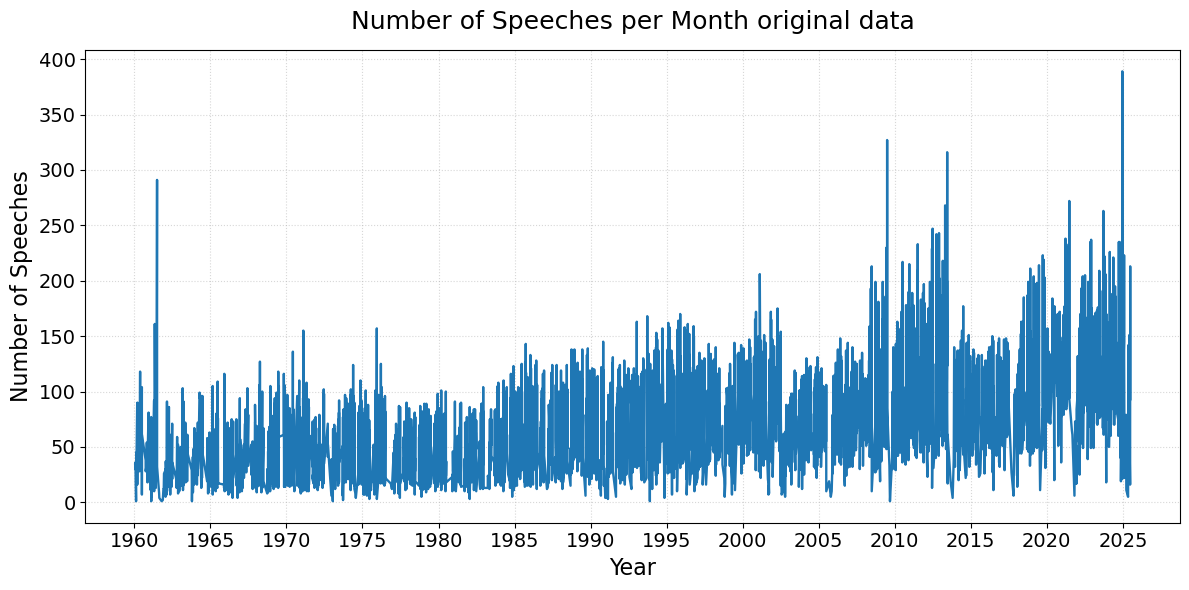
\includegraphics[width=12cm]{images/originalDataDistributionMonthly.png}
    		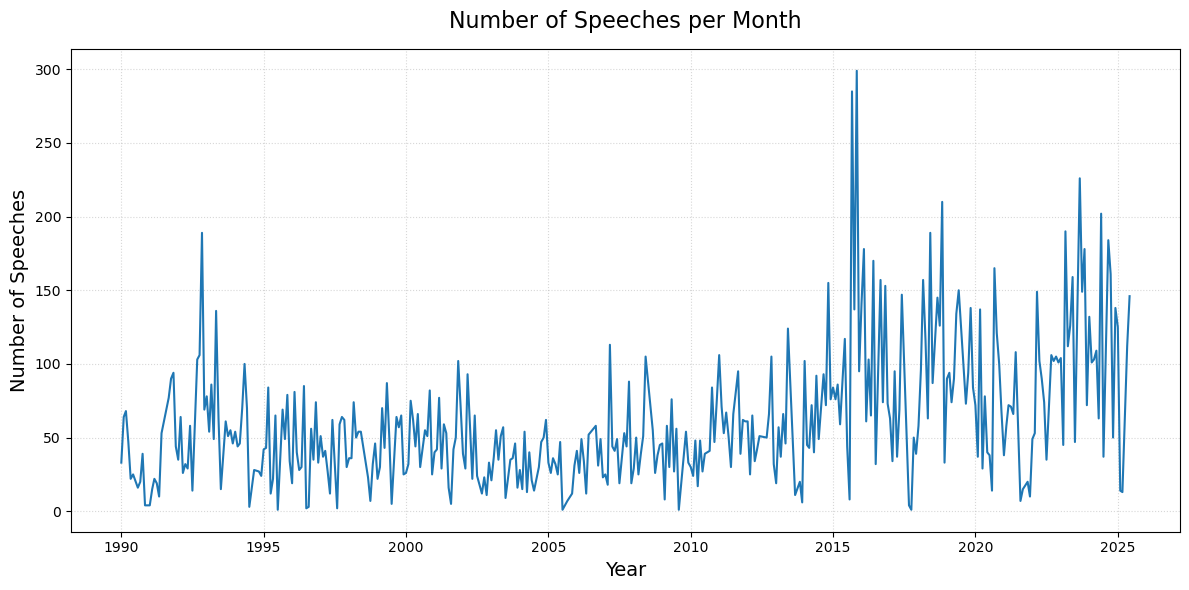
\includegraphics[width=12cm]{images/FilterDataDistributionMonthly.png}
    		\caption{Monthly number of parliamentary speeches (top: original data; bottom: immigration-related speeches after keyword filtering).}
    		\label{filtereddataplot}
    	\end{center}
    \end{figure}
    
    To make sentiment scores easier to interpret, and to reduce computing time, we keep only speeches that clearly discuss immigration. We identify these using keyword filtering, based on the keyword list from \textcite{kostikova2024fine}. Since our filter uses Python's \texttt{re} module for pattern matching, we merge word forms that share the same root (e.g., \textit{Flüchtling}, \textit{Flüchtlinge}, \textit{Flüchtlingen}) into a single stem, so no two entries overlap. This reduces the original list of 32 word forms (Table~\ref{tab:keywords-original}) to 13 stems covering the same meaning without duplication (Table~\ref{tab:keywords-stems}).
    
    \begin{table}[htbp]
    	\centering
    	\caption{Original keyword list (32 inflected word forms), following \textcite{kostikova2024fine}.}
    	\label{tab:keywords-original}
    	\footnotesize
    	\begin{tabular}{llll}
    		\toprule
    		\multicolumn{4}{c}{Keywords} \\
    		\midrule
    		Flüchtlinge & Ausländer & Flüchtlingen & Zuwanderung \\
    		Vertriebenen & Ausländern & Asylbewerber & Migranten \\
    		Migration & Heimatvertriebenen & Aussiedler & Einwanderung \\
    		Ansiedler & Vertriebene & Zuwanderer & Asylbewerbern \\
    		Flüchtling & Heimatvertriebene & Sowjetzonenflüchtlinge & Aussiedlern \\
    		Einwanderer & Asylsuchenden & Asylsuchende & Bürgerkriegsflüchtlinge \\
    		Zuwanderern & Ansiedlern & Migrantinnen & Vertriebener \\
    		Emigranten & Kriegsflüchtlinge & Ausländerinnen & Immigranten \\
    		\bottomrule
    	\end{tabular}
    \end{table}
    
    \begin{table}[htbp]
    	\centering
    	\caption{Reduced list of 13 word stems used for regular-expression matching. Word forms sharing a root were merged into one stem, so no entry overlaps with another.}
    	\label{tab:keywords-stems}
    	\footnotesize
    	\begin{tabular}{llll}
    		\toprule
    		\multicolumn{4}{c}{Word stems} \\
    		\midrule
    		\texttt{migration} & \texttt{zuwander} & \texttt{einwander} & \texttt{asyl} \\
    		\texttt{fluechtling} & \texttt{gefluechtet} & \texttt{schutzsuchend} & \texttt{auslaend} \\
    		\texttt{vertrieben} & \texttt{migrant} & \texttt{aussiedler} & \texttt{ansiedler} \\
    		\texttt{buergerkriegs} & & & \\
    		\bottomrule
    	\end{tabular}
    \end{table}
    
    This filtering reduces the corpus from 260,660 to 28,662 speeches, about 11\% of all speeches. Figure~\ref{filtereddataplot} shows the counts before and after filtering. While total speeches have grown steadily over time, immigration-related speeches have grown even more, especially during periods of high migration.
    
    From this reduced corpus, we build two sentiment dictionaries: a welcoming (open) dictionary and a restrictive dictionary. We build them in three steps: manual seed selection, Word2Vec-based expansion, and manual cleaning.
    
    \paragraph{Step 1: Manual seed selection.} We manually pick speeches that reflect different immigration positions, based on the documented history of German parties on this issue: 200 AfD speeches from 2017--2025, 94 CDU/CSU speeches from 1990--1994, and 500 CDU/CSU, SPD, and FDP speeches from the 2015--2018 refugee period. Close reading of these speeches gives us 655 seed words for the welcoming dictionary and 872 for the restrictive dictionary.
    
    \paragraph{Step 2: Word2Vec-based expansion.} We train a skip-gram Word2Vec model on the immigration-related corpus (vector size 100, context window 7, minimum word count 10, 50 training epochs, fixed random seed). We expand the dictionaries iteratively: in each round, we use a small, topic-focused seed list (for example, terms about the economic side of migration policy). For each seed word in the model's vocabulary, we find its 20 nearest neighbors by cosine similarity. We keep a candidate word only if (i) its similarity to the seed is at least 0.72, (ii) it appears in a \ac{TF-IDF} vocabulary built on the immigration corpus ($\mathit{max\_features}=80{,}000$, $\mathit{min\_df}=2$), and (iii) it is a purely alphabetic token longer than three characters. Words that appear as neighbors of seeds from both dictionaries are treated as ambiguous and dropped from both. We merge the kept words from each round into the growing dictionaries, ending with 755 welcoming words and 968 restrictive words.
    
    \begin{figure}[h]
    	\begin{center}
    		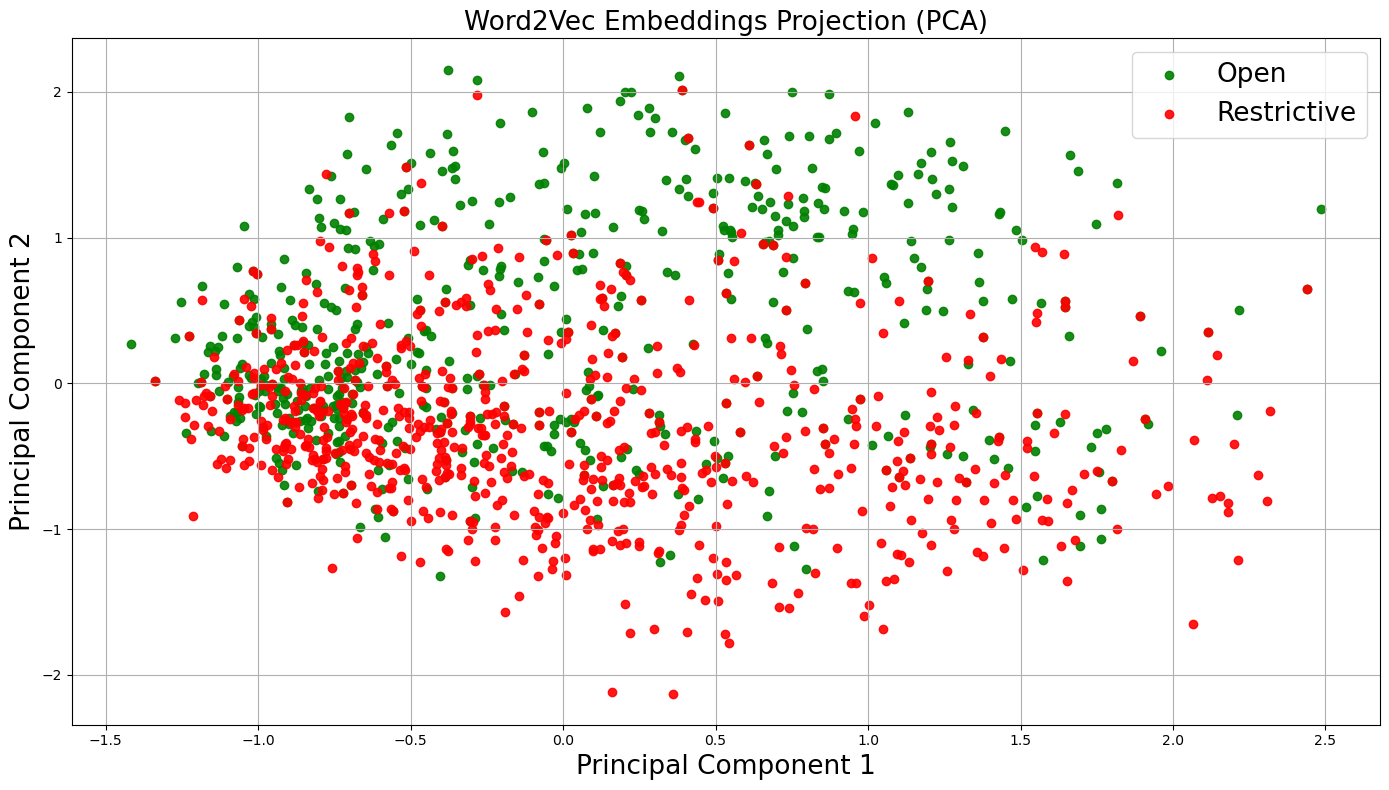
\includegraphics[width=12cm]{images/wordtwovectone.png}
    		\caption{PCA projection of the expanded immigration dictionaries before cleaning (restrictive = red, welcoming = green).}
    		\label{wordtwovecone}
    	\end{center}
    \end{figure}
    
    To sharpen the split between the two dictionaries, we project the word embeddings onto two dimensions using \ac{PCA}, which keeps most of the variance while giving an interpretable view of the embedding space. As Figure~\ref{wordtwovecone} shows, restrictive terms (red) mostly sit lower in the projection, while welcoming terms (green) sit higher. The interval $[-0.48, 0.5]$ on the $y$-axis holds most ambiguous words. We keep restrictive words with a $y$-coordinate below $-0.48$ and welcoming words above $0.5$, dropping everything in between. This gives cleaner dictionaries (Figure~\ref{wordtwovecttwo}) of 288 restrictive and 241 welcoming terms.
    
    \begin{figure}[h]
    	\begin{center}
    		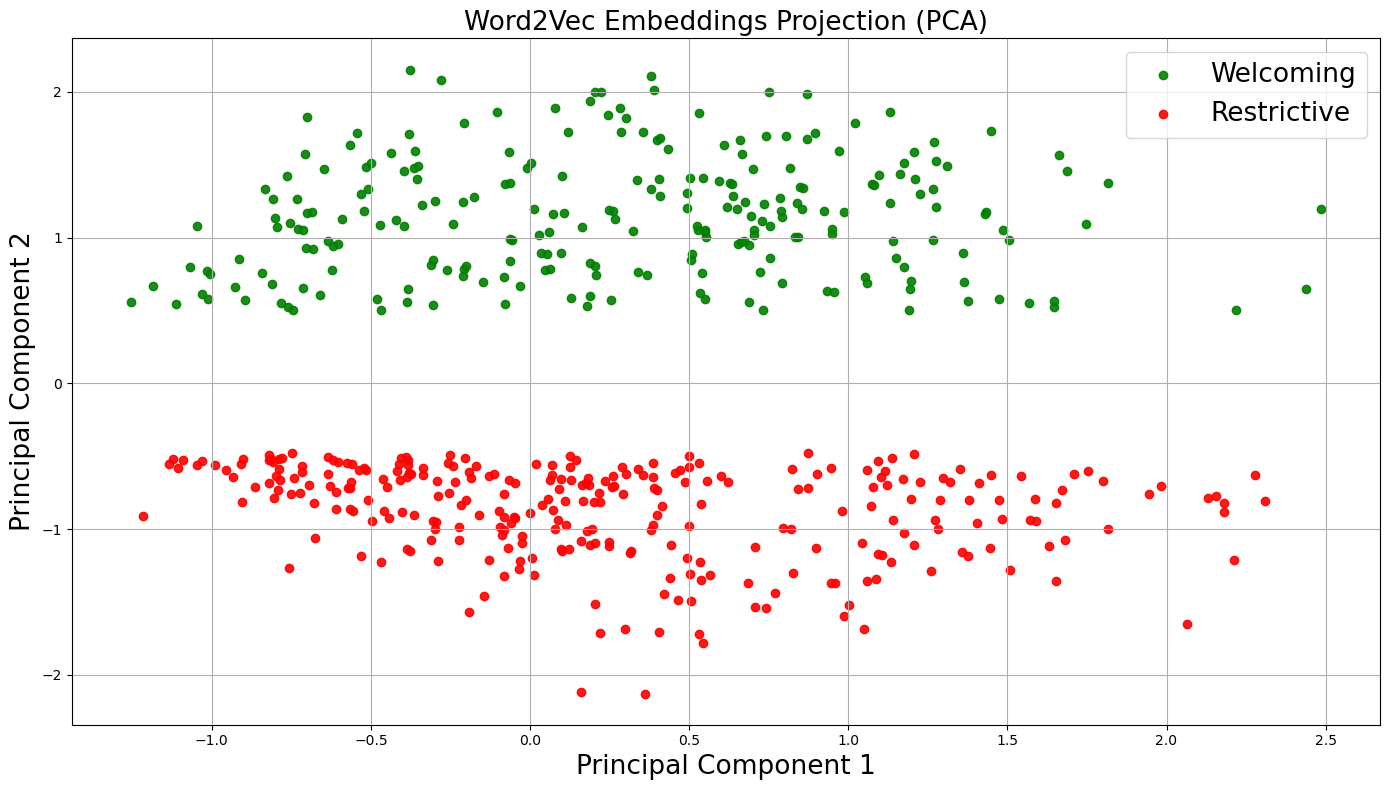
\includegraphics[width=12cm]{images/wordtwovecttwo.png}
    		\caption{PCA projection of the refined dictionaries after $y$-coordinate threshold cleaning (restrictive = red, welcoming = green), showing clearer separation between the two stances.}
    		\label{wordtwovecttwo}
    	\end{center}
    \end{figure}
    
    \paragraph{Step 3: Manual cleaning.} \label{sec:party_averages} We then manually clean the dictionaries, prompted by an early check of average sentiment scores by party (Section~\ref{sentiment-index-construction}). This check found implausibly negative scores for parties known to hold welcoming positions, especially Bündnis~90/Die Grünen and Die Linke. For each of these parties, we randomly sampled speeches with a sentiment score below zero and read them individually.
    
    This revealed two problems. First, restrictive words were sometimes used critically, for example when a speaker quoted or condemned anti-immigration rhetoric rather than expressing it themselves — a nuance our embedding-based measure cannot capture. Second, some dictionary words carried purely administrative or legal meaning (e.g., \textit{Familiennachzug}, \textit{Asylrecht}, \textit{Ausländer}) or no clear stance at all (e.g., \textit{abschieben}, \textit{Abschiebung}, \textit{Zurückweisung}, \textit{Migrationswelle}, \textit{Migrationsstrom}), adding noise unrelated to the speaker's actual position. We removed all such entries, retrained the model, and recomputed the scores.
    
    This cleaning was not done to force parties into a preset ranking: after this step, Bündnis~90/Die Grünen's average sentiment became less negative, while Die Linke's stayed negative (Figure~\ref{AveragePartySentiment}). This shows the correction came from real misclassifications found by close reading, not from adjusting until a target ranking appeared. We revisit this in the robustness check (Section~\ref{sec:robustness}).
    
    This gives a final welcoming dictionary of 222 words, covering skilled labor, the economy, the labor market, human rights, humanitarian aid, protection, integration, education, language learning, citizenship, social cohesion, and diversity and inclusion. The final restrictive dictionary has 178 words, covering border security, state control, repatriation, deportation, legal enforcement, capacity limits, labor market protection, and concerns about social integration \footnote{To conserve space in the main document, the complete lists of welcoming and restrictive dictionary terms are provided in the replication code and supplementary data folder accompanying this thesis.}.
    
    \begin{table}[htbp]
    	\centering
    	\caption{Evolution of the welcoming and restrictive vocabularies}
    	\label{tab:vocabulary_evolution}
    	\begin{tabular}{lrrr}
    		\toprule
    		\textbf{Stage} & \textbf{Welcoming} & \textbf{Restrictive} & \textbf{Total} \\
    		\midrule
    		Initial seeds & 655 & 872 & 1527 \\
    		Word2Vec expansion & 755 & 969 & 1724 \\
    		PCA refinement & 241 & 288 & 529 \\
    		Final vocabulary & 222 & 178 & 400 \\
    		\bottomrule
    	\end{tabular}
    \end{table}
    
    \subsection{Sentiment Index Construction}
    \label{sentiment-index-construction}
    
    We build an immigration sentiment index from the reduced corpus. To capture semantic similarity in natural language, we need a method that turns sentences, paragraphs, and whole documents into numeric vectors while keeping their meaning. Since our corpus has thousands of speeches, Doc2Vec is a good fit: it is an unsupervised, neural-network method that learns vector representations of documents in a high-dimensional space \parencite{le2014distributed}.
    
    \begin{figure}[h]
    	\begin{center}
    		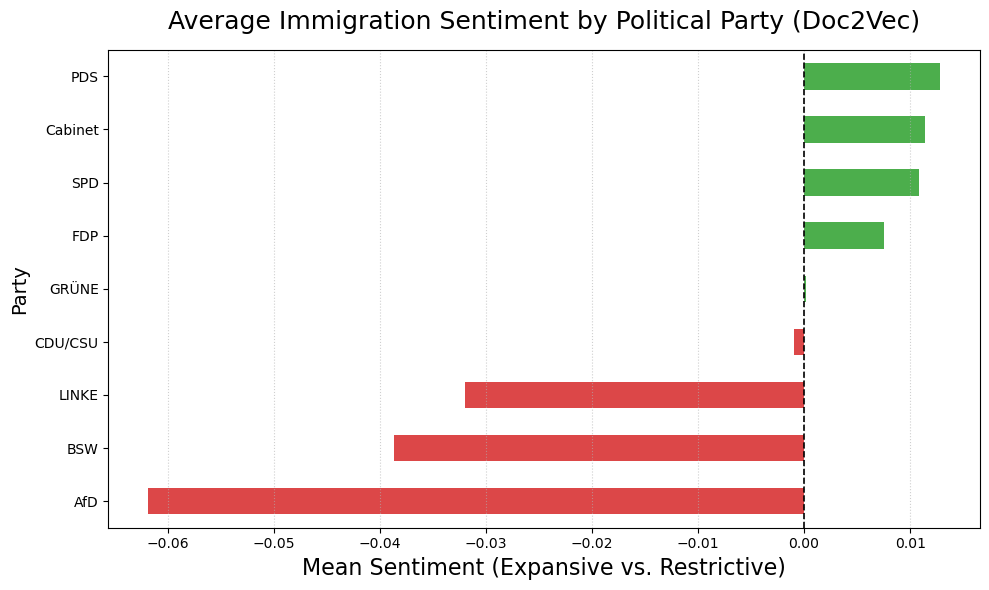
\includegraphics[width=12cm]{images/averagePartySentiment.png}
    		\caption{Average restrictive immigration sentiment by political party (negative values indicate frequent use of restrictive anti-immigration vocabulary, whether framed defensively or critically).}
    		\label{AveragePartySentiment}
    	\end{center}
    \end{figure}
    
    Instead of simply counting dictionary words, we embed both speeches and dictionary terms in one shared vector space, and define each speech's stance as its cosine similarity to two reference vectors — one per dictionary. We use a rolling-window Doc2Vec procedure to avoid look-ahead bias: speeches in a given quarter are always scored using a model trained only on earlier data.
    
    For each quarter $t$, we train a \ac{PV-DBOW} Doc2Vec model (\texttt{dm=0}, with word vectors trained jointly via \texttt{dbow\_words=1}), vector size 100, context window 5, minimum word count 1, initial learning rate 0.025, and 50 training epochs, using only speeches from the preceding 40 quarters (ten years), $[t-40, t)$. This follows the rolling-window design of \textcite{latifi2024fiscal} for fiscal sentiment, adapted here for immigration. Figure~\ref{rollingwindow} shows the procedure.
    
    Using this model, we build two reference vectors — one for each dictionary — by averaging the embeddings of all dictionary words present in that window's vocabulary (for multi-word entries, we sum the word embeddings). We then infer document vectors for all speeches in the following, held-out quarter $t$, and compute their cosine similarity to each reference vector, giving a \textit{similarity\textsubscript{welcoming}} and a \textit{similarity\textsubscript{restrictive}} score per speech.
    
    We start the rolling training from Q1 1980 onward, since immigration-related discourse becomes more consistent from this point. With the ten-year window requirement, this gives out-of-sample sentiment scores from Q1 1990 to Q2 2025.
    
    The sentiment score of speech $i$ is the difference between its two similarities:
    \begin{equation}
    	\text{sentiment}_i = \text{similarity}_{\text{welcoming},i} -
    	\text{similarity}_{\text{restrictive},i}.
    	\label{eq:sentiment_score}
    \end{equation}
    
    A positive score means a speech is closer to the welcoming reference vector; a negative score means the opposite.
    
    \begin{figure}[h]
    	\begin{center}
    		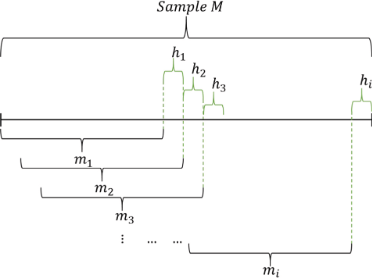
\includegraphics[width=8cm]{images/rollingwindow.png}
    		\caption{Rolling-window estimation for the Doc2Vec model. The corpus is split into fixed training windows ($m$) and following inference windows ($h$), shifted forward by one period each time. Adapted from \textcite{latifi2024fiscal}.}
    		\label{rollingwindow}
    	\end{center}
    \end{figure}
    
    \subsection{Validation of the Sentiment Measure}
    \label{validation-of-the-sentiment-measure}
    
    \begin{figure}[h]
    	\begin{center}
    		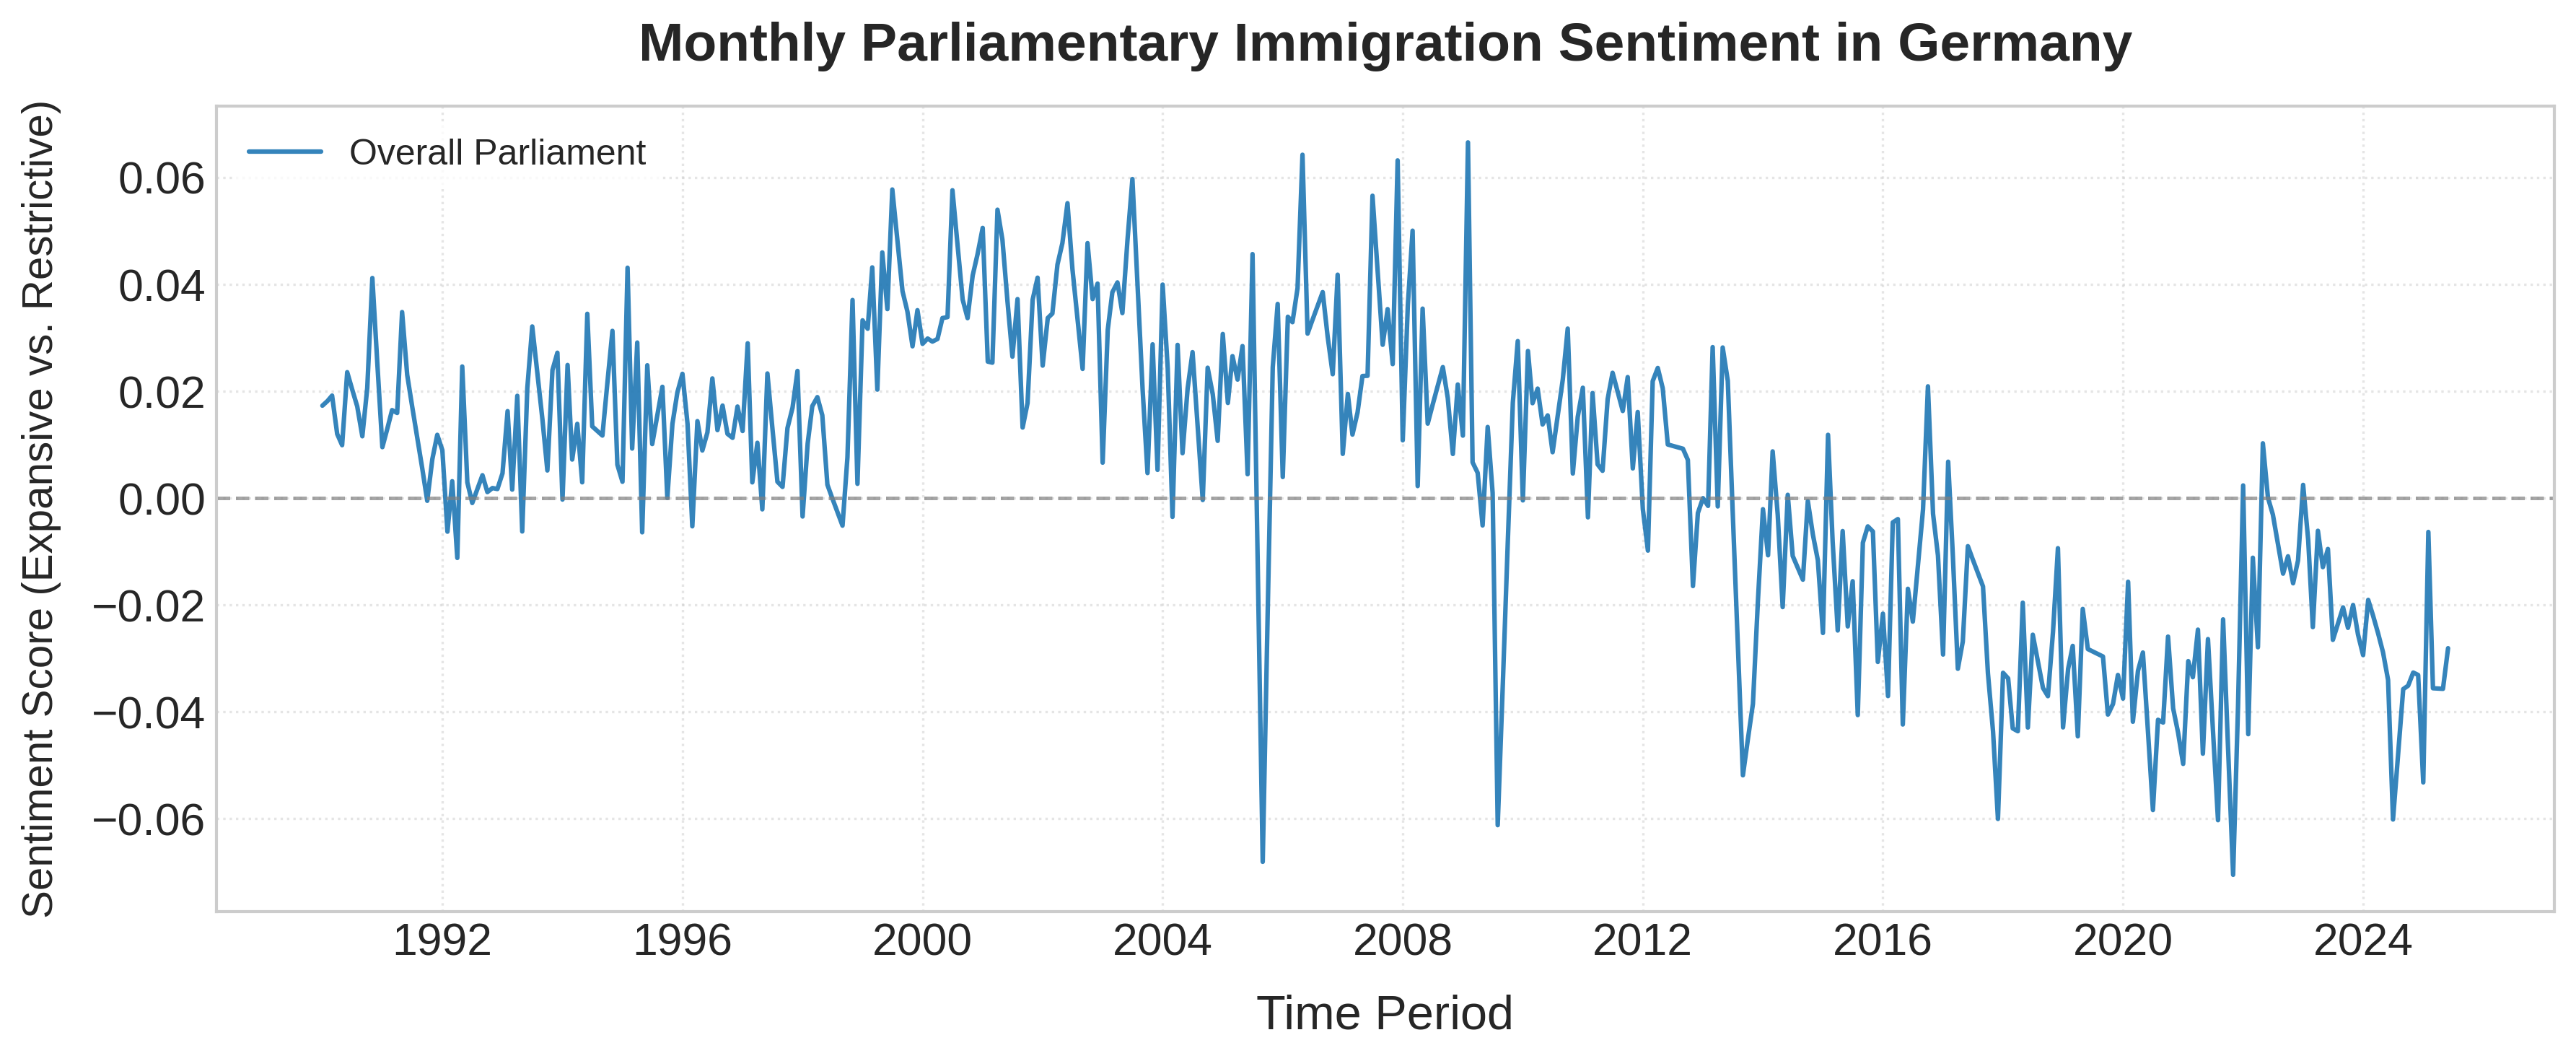
\includegraphics[width=15cm]{images/foursentiment.png}
    		\caption{Monthly trend of overall parliamentary immigration sentiment in Germany. Positive scores show a net-expansive vocabulary; negative scores show more restrictive terminology (whether defensive or critical).}
    		\label{overallsentiment}
    	\end{center}
    \end{figure}
    
    \begin{figure}[h]
    	\begin{center}
    		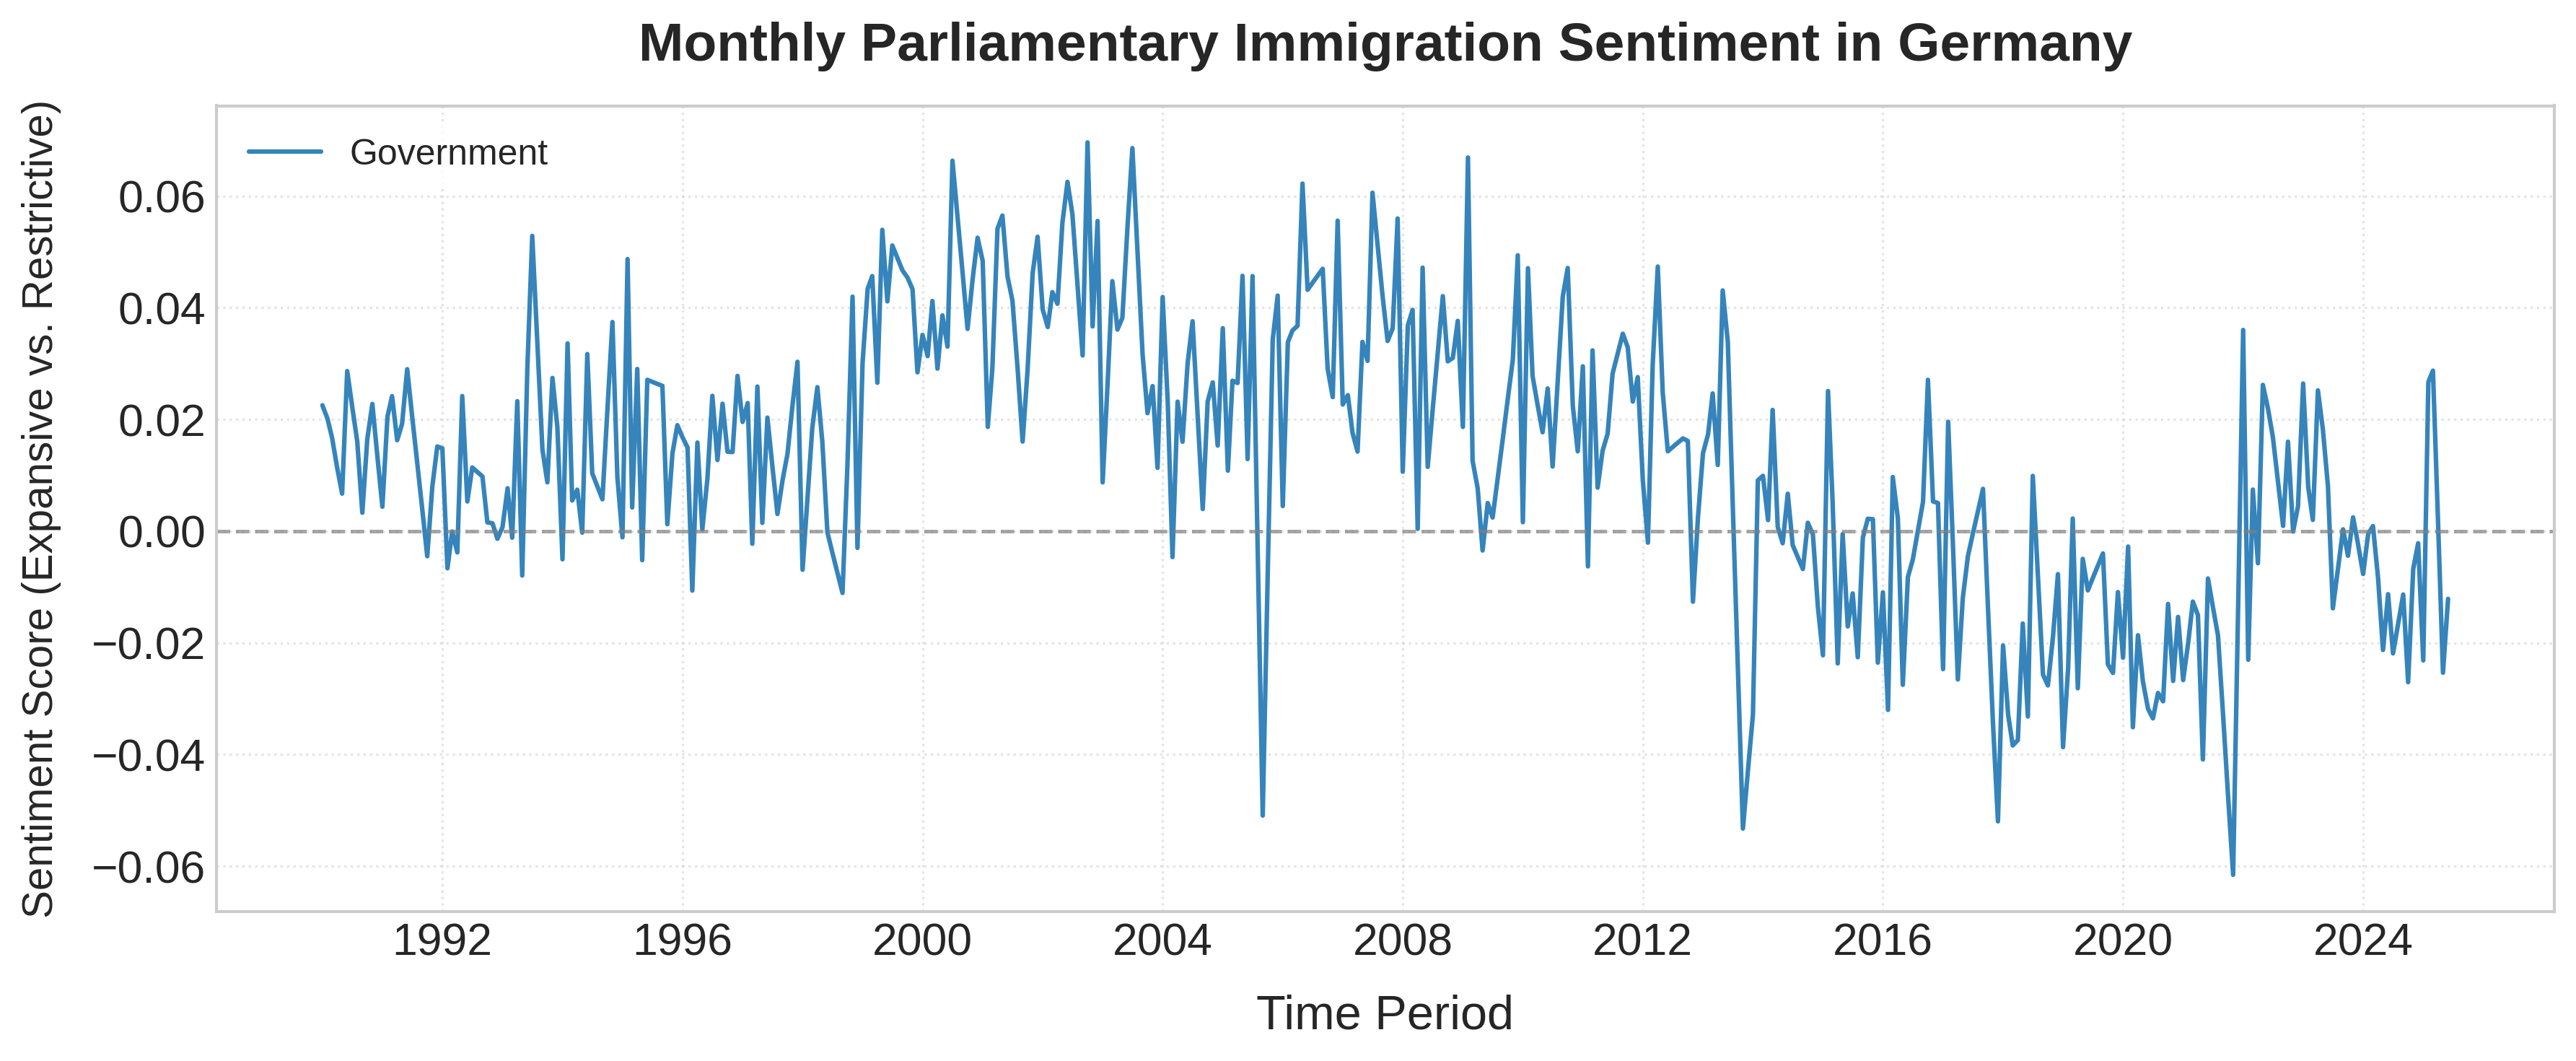
\includegraphics[width=13cm]{images/sentimentgorvnment.png}
    		\caption{Monthly trend of government parliamentary immigration sentiment in Germany.}
    		\label{sentimentgovermment}
    	\end{center}
    \end{figure}
    
    We check the plausibility of our sentiment measure by comparing it to well-known shifts in German immigration politics. A close match between the estimated series and known historical events is qualitative evidence that the measure captures real variation in political discourse, not just noise.
    
    Overall sentiment shows two broad phases: mostly positive from 1990 to 2014, then clearly negative from 2014 onward (Figure~\ref{overallsentiment}). Government and opposition sentiment move together for most of the period, diverging mainly around 2006--2007 and 2018--2022 (Figure~\ref{allsentiment}).
    
    A clear dip appears between 1992 and 1994, matching the more restrictive rhetoric of that time aimed at reducing asylum applications \parencite{borkert2007migration}. Sentiment turns more positive around 2000, matching the introduction of birthright citizenship (jus soli) and the Süssmuth Commission's work \parencite{borkert2007migration}. Between 2014 and 2021, government sentiment swings more sharply (Figure~\ref{sentimentgovermment}), while opposition sentiment trends more negative (Figure~\ref{sentimentopposition}) — patterns credibly linked to the Syrian refugee crisis \parencite{trauner2017welcome}, the COVID-19 pandemic, and the 2021 federal election, where immigration was a major campaign topic and public debate turned more restrictive. The positive peak in overall sentiment in 2022 (Figure~\ref{overallsentiment}) realistically reflect solidarity with Ukrainian refugees \parencite{brucker2022war}.
    
    \begin{figure}[h]
    	\begin{center}
    		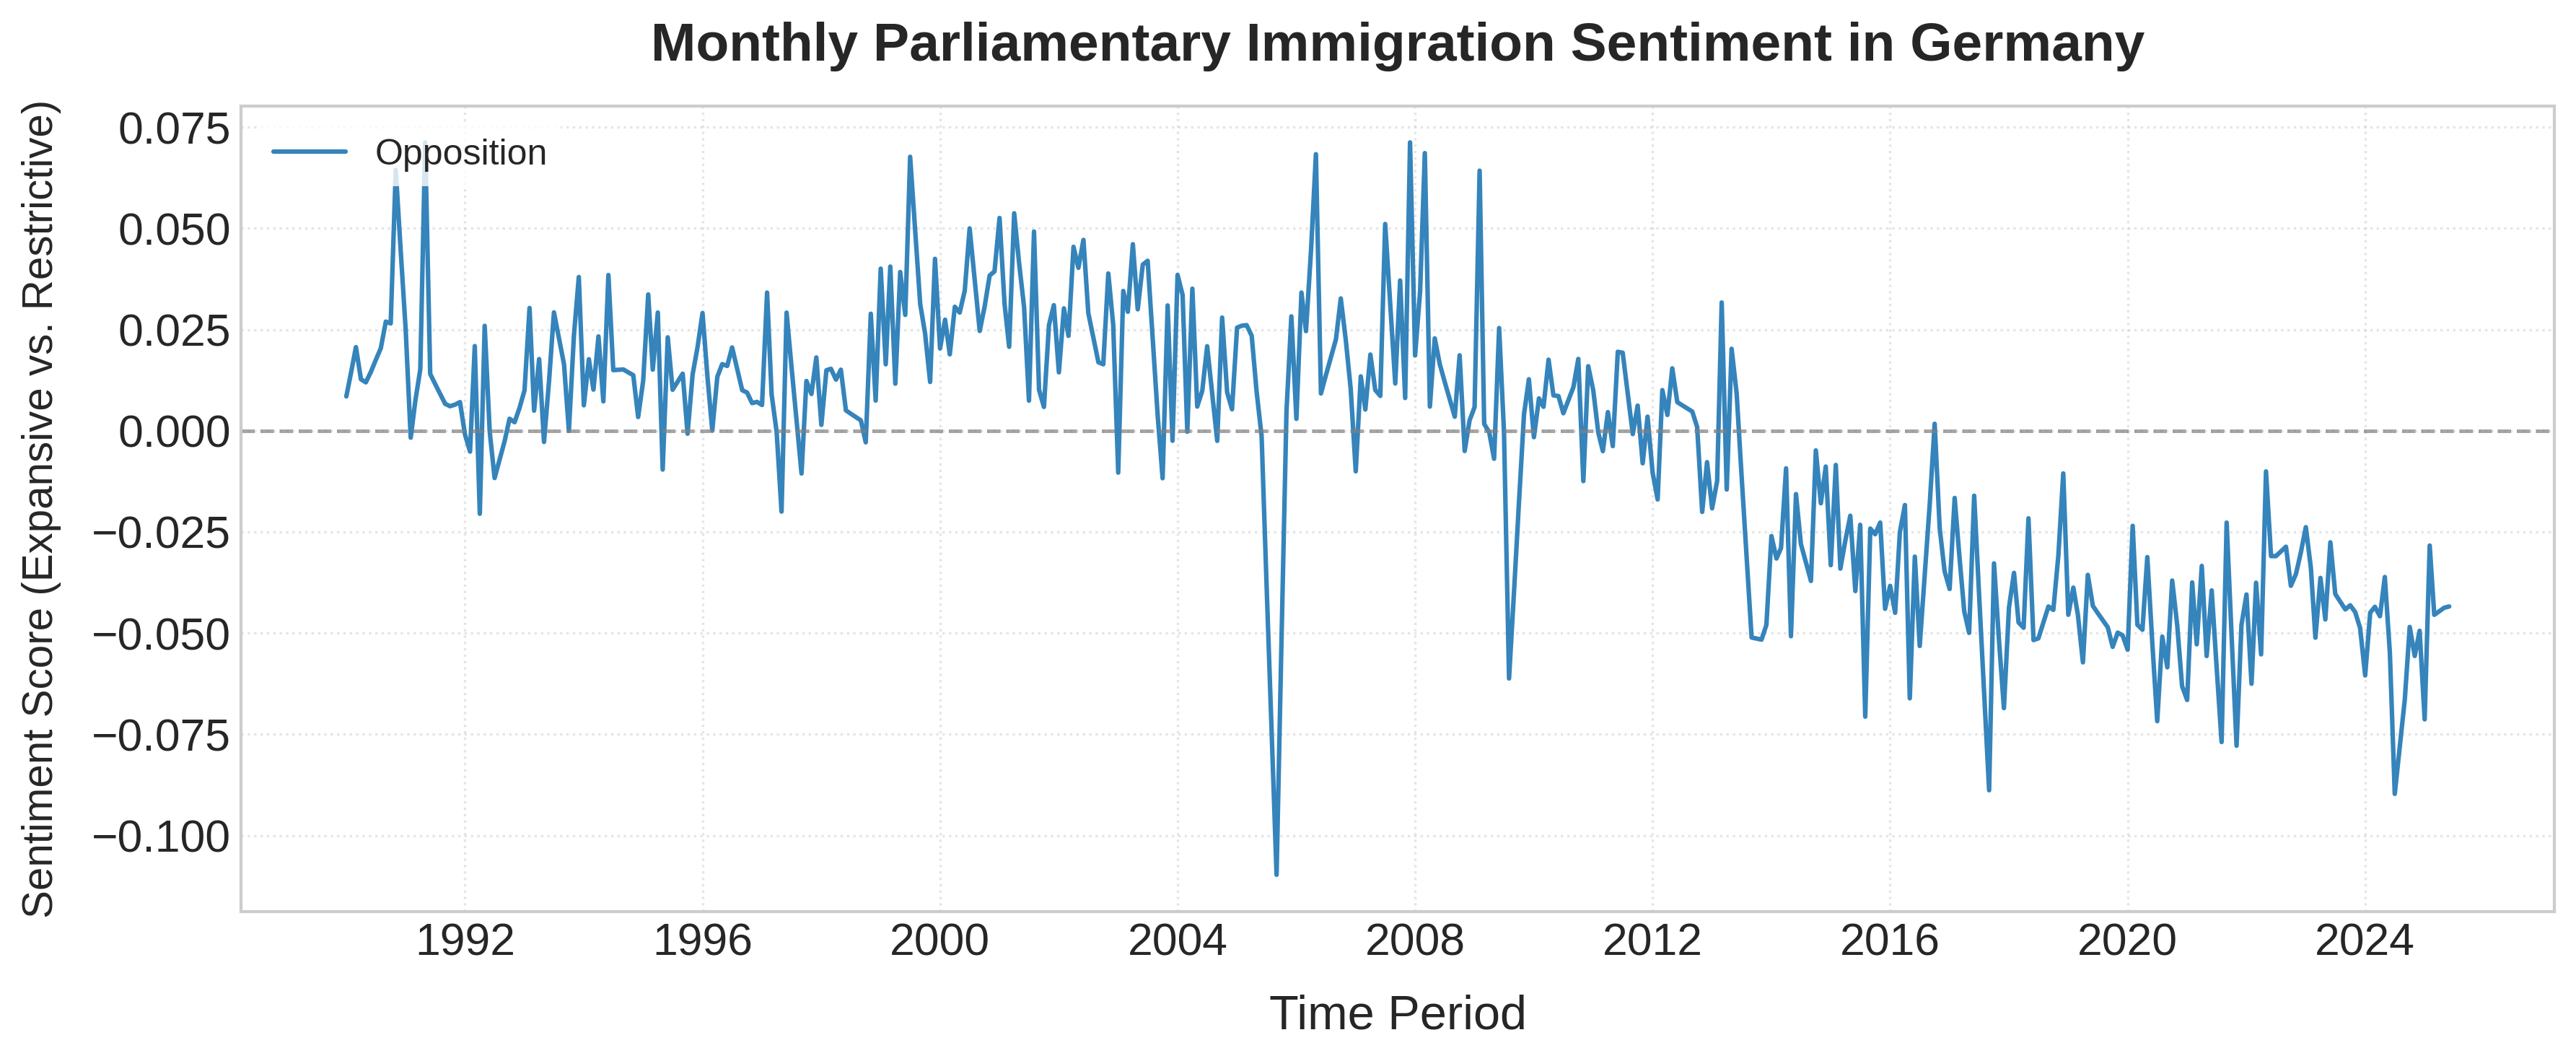
\includegraphics[width=13cm]{images/sentimentOpposition.png}
    		\caption{Monthly trend of opposition parliamentary immigration sentiment in Germany.}
    		\label{sentimentopposition}
    	\end{center}
    \end{figure}
    
    \begin{figure}[h]
    	\begin{center}
    		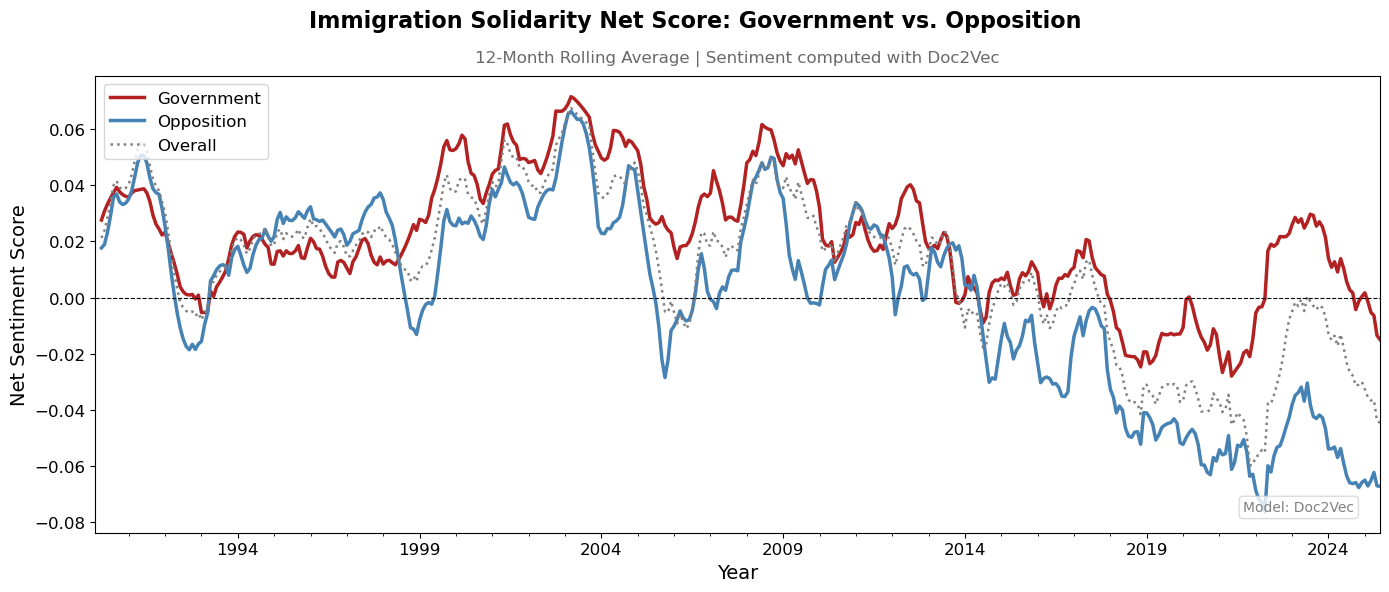
\includegraphics[width=13cm]{images/allSentimentTogether.png}
    		\caption{Monthly trend of immigration sentiment for the overall parliament, government, and opposition in Germany.}
    		\label{allsentiment}
    	\end{center}
    \end{figure}
    
    Party-level results show large differences in immigration-related discourse. The AfD shows mostly negative sentiment throughout its observed period, while parties traditionally seen as pro-immigration show higher average scores, though variation within each party remains substantial (Appendix~\ref{fig:party_sentiment}).
  
    \newpage
    
%    % ----------------------------------------------------------------
    \section{Estimating the macroeconomic effects}
    \label{sec:economic_interaction}
    We now investigate the macroeconomic effects of immigration sentiment as reflected in the textual data. For that purpose, we augment the baseline VAR model from the study \parencite{maffei2021does} by our new sentiment series.
    
    \subsection{VAR Model}
     
     This study employs a Bayesian vector autoregressive (VAR) framework to
     analyse the dynamic relationships among the selected macroeconomic and
     political variables. The model is estimated over different sample periods in
     order to examine the robustness of the results and to distinguish between the
     pre-pandemic and extended sample periods. Specifically, the analysis considers
     the periods 2006--2019, 2007--2019, and 2007--2025.
     
     For the pre-pandemic samples, namely 2006--2019 and 2007--2019, we estimate
     a standard reduced-form VAR model with $p$ lags and $n$ endogenous variables:
     
     \begin{equation}
     	\mathbf{y}_t = \boldsymbol{\mu} + \mathbf{A}_1\mathbf{y}_{t-1} + \cdots +
     	\mathbf{A}_p\mathbf{y}_{t-p} +\mathbf{u}_t,\end{equation}
     
     where $\mathbf{y}_t$ denotes an $n \times 1$ vector of endogenous variables,
     $\boldsymbol{\mu}$ is an $n \times 1$ vector of intercept terms, and
     $\mathbf{A}_i$, for $i=1,\ldots,p$, are $n \times n$ autoregressive
     coefficient matrices. The reduced-form disturbance vector $\mathbf{u}_t$ is
     assumed to follow a multivariate normal distribution,
     
     \begin{equation}\mathbf{u}_t \sim \mathcal{N}(\mathbf{0},\boldsymbol{\Sigma}), \end{equation}
     
     where $\boldsymbol{\Sigma}$ is a positive-definite $n \times n$
     variance--covariance matrix satisfying
     
     \begin{equation}
     	E(\mathbf{u}_t\mathbf{u}_t')
     	= \boldsymbol{\Sigma}. \end{equation}
     
     The reduced-form disturbances are assumed to be serially uncorrelated at all
     non-zero leads and lags.
     
     For the extended sample covering the period 2007--2025, the baseline VAR
     specification is augmented by an exogenous COVID-19 dummy variable in order
     to account for the exceptional economic and social disturbances associated
     with the pandemic. The extended model is therefore specified as
     
     \begin{equation}
     	\mathbf{y}_t
     	= \boldsymbol{\mu} + \mathbf{A}_1\mathbf{y}_{t-1} + \cdots + \mathbf{A}_p\mathbf{y}_{t-p} + \mathbf{B}\mathbf{x}_t + \mathbf{u}_t,
     \end{equation}
     
     where $\mathbf{x}_t$ denotes the vector of exogenous variables and
     $\mathbf{B}$ contains the corresponding coefficients. In the present
     application, $\mathbf{x}_t$ consists of a single COVID-19 dummy variable,
     such that 
      \begin{equation}
     	\mathit{COVID}_t =
     	\begin{cases}
     		1, & \text{for observations between March 2020 and October 2021}, \\
     		0, & \text{otherwise}.
     	\end{cases}
     	\label{eq:covid_dummy}
     \end{equation}
     
     The COVID-19 dummy is included only in the estimation based on the
     2007--2025 sample. It is treated as an exogenous control variable and does
     not form part of the endogenous VAR system. Consequently, it does not enter
     the autoregressive dynamics represented by the coefficient matrices
     $\mathbf{A}_1,\ldots,\mathbf{A}_p$.
     The VAR model can be written in compact matrix form as
     \begin{equation}
     	\mathbf{Y} = \mathbf{X}\mathbf{\Pi} + \mathbf{U}, \end{equation}
     where
     \begin{equation} \mathbf{Y} = \left( \mathbf{y}_{p+1}, \ldots,\mathbf{y}_{T}
     	\right)'\end{equation}
     is a $(T-p) \times n$ matrix containing the observations of the endogenous
     variables.
 
     For the baseline VAR specification, the regressor matrix is given by    
     \begin{equation}
     	\mathbf{X} = \left( \mathbf{1}, \mathbf{Y}_{-1}, \ldots, \mathbf{Y}_{-p}
     	\right),\end{equation}
     where $\mathbf{1}$ is a $(T-p) \times 1$ vector of ones and
     \begin{equation} \mathbf{Y}_{-j} = \left( \mathbf{y}_{p+1-j}, \ldots,
     	\mathbf{y}_{T-j} \right)'\end{equation}
     is a $(T-p) \times n$ matrix containing the $j$th lag of the endogenous
     variables. Thus, in the baseline specification, $\mathbf{X}$ has dimension
     \begin{equation} (T-p) \times (1+np).\end{equation}
     
     For the extended 2007--2025 specification, the exogenous COVID-19 dummy is
     included in the regressor matrix:
     \begin{equation}
     	\mathbf{X} = \left(\mathbf{1},\mathbf{X}_{COVID},\mathbf{Y}_{-1},\ldots,
     	\mathbf{Y}_{-p} \right).\end{equation}
     
     Since only one exogenous variable is included, the corresponding regressor
     matrix has dimension
     \begin{equation} (T-p) \times (2+np).\end{equation}
     
     More generally, with $k$ exogenous variables, the dimension of the regressor
     matrix is $(T-p) \times (1+k+np)$.
     
     The coefficient matrix for the baseline specification is defined as
     \begin{equation}
     	\mathbf{\Pi} = \left( \boldsymbol{\mu}, \mathbf{A}_1,\ldots,\mathbf{A}_p
     	\right)',\end{equation}
     
     whereas, for the extended specification including the COVID-19 dummy, it is
     given by
     \begin{equation}
     	\mathbf{\Pi} = \left(\boldsymbol{\mu},\mathbf{B},\mathbf{A}_1,\ldots,
     	\mathbf{A}_p \right)'.\end{equation}
     The error matrix is defined as
     \begin{equation}
     	\mathbf{U} = \left(\mathbf{u}_{p+1},\ldots,\mathbf{u}_{T}\right)',
     \end{equation}
     and has dimension $(T-p) \times n$.
     We estimate the VAR model using the variables in levels. The KPSS results indicate that most variables are non-stationary in levels (see Tables~\ref{tab:kpss_level} and~\ref{tab:kpss_level_dataset2}), while the Johansen trace test provides evidence of long-run relationships among the variables (see Tables~\ref{tab:johansen_trace} and~\ref{tab:johansen_trace_dataset2} in the Appendix). Given the objective of preserving these long-run relationships and following the level-VAR approach adopted in the reference study, the VAR models are estimated in levels. The resulting impulse responses are therefore interpreted primarily as dynamic associations rather than as estimates of a structural causal mechanism (\cite{sims1990inference}).
         
     \subsubsection{Bayesian Estimation}
     
     Both the baseline VAR models and the extended specification including the
     COVID-19 dummy are estimated within a Bayesian framework. 
     
     Lag length was assessed using the Akaike Information Criterion (AIC),
     Hannan--Quinn Information Criterion (HQ), Schwarz Information Criterion
     (SC), and Final Prediction Error (FPE). As shown in
     Table~\ref{tab:lag_selection}, the criteria disagree substantially: AIC
     and FPE favor long lag structures, particularly in the 2007--2019 and
     2007--2014 sub-samples, while SC consistently favors one or two lags
     across all samples. We follow the Schwarz Criterion throughout, both
     for its parsimony and to guard against overfitting given the limited
     sample size. This yields one monthly lag for the original 2006--2019
     specification, two lags for the reconstructed 2007--2025 sample, and
     one lag for the reconstructed 2007--2019 and 2007--2014 sub-samples.
     
     \begin{table}[htbp]
     	\centering
     	\caption{VAR Lag Length Selection}
     	\label{tab:lag_selection}
     	\begin{tabular}{lrrrrc}
     		\hline
     		\textbf{Sample} & \textbf{AIC} & \textbf{HQ} &
     		\textbf{SC} & \textbf{FPE} & \textbf{Final Lag (SC)} \\
     		\hline
     		Original study (2006--2019) & 3 & 2 & 1 & 3 & 1 \\
     		Reconstructed, 2007--2025   & 3 & 3 & 2 & 3 & 2 \\
     		Reconstructed, 2007--2019   & 10 & 2 & 1 & 9 & 1 \\
     		Reconstructed, 2007--2014   & 5 & 2 & 1 & 4 & 1 \\
     		\hline
     	\end{tabular}
     	
     	\begin{flushleft}
     		\footnotesize
     		\textit{Notes:} AIC denotes the Akaike Information Criterion,
     		HQ the Hannan--Quinn Information Criterion, SC the Schwarz
     		Information Criterion, and FPE the Final Prediction Error.
     		Reported values indicate the lag order minimizing each
     		criterion. The lag order selected by SC is retained in the
     		final specification for each sample.
     	\end{flushleft}
     \end{table}
     
     The objective is to generate posterior draws (one thousand) of the coefficient matrix $\mathbf{\Pi}$ and the covariance matrix $\boldsymbol{\Sigma}$ from their joint posterior distribution. According to Bayes' theorem, the joint posterior distribution is proportional to the likelihood of the observed data multiplied by the
     prior distributions:
     \begin{equation}
     	p(\mathbf{\Pi},\boldsymbol{\Sigma}
     	\mid
     	\mathbf{Y},\mathbf{X})
     	\propto
     	p(\mathbf{Y}
     	\mid
     	\mathbf{X},\mathbf{\Pi},\boldsymbol{\Sigma})
     	p(\mathbf{\Pi}\mid\boldsymbol{\Sigma})
     	p(\boldsymbol{\Sigma}).
     \end{equation}
     Following a non-informative Bayesian approach, a flat prior is assigned to
     the coefficient matrix,
     \begin{equation}
     	p(\mathbf{\Pi}\mid\boldsymbol{\Sigma})
     	\propto
     	1,
     \end{equation}
     while the covariance matrix is assigned the Jeffreys prior,
     \begin{equation}
     	p(\boldsymbol{\Sigma})
     	\propto
     	|\boldsymbol{\Sigma}|^{-(n+1)/2}.
     \end{equation}
     Posterior simulation is carried out by drawing from the corresponding
     conditional posterior distributions of $\mathbf{\Pi}$ and
     $\boldsymbol{\Sigma}$. By repeating this procedure thousands of times, we obtain posterior draws from the joint posterior distribution. A detailed derivation of the
     posterior distributions and a description of the Bayesian estimation
     procedure can be found in \textcite{maffei2021does}.
   
    \subsubsection{Structural Identification}
    
    The reduced-form disturbances $\mathbf{u}_t$ are generally contemporaneously
    correlated. Therefore, a structural identification scheme is required in
    order to interpret the innovations as economically meaningful shocks. The
    relationship between the reduced-form disturbances and the structural
    disturbances is given by 
    \begin{equation}
    	\mathbf{u}_t
    	=
    	\mathbf{S}\boldsymbol{\varepsilon}_t,
    \end{equation}
    where $\boldsymbol{\varepsilon}_t$ is an $n \times 1$ vector of structural
    disturbances satisfying
    \begin{equation}
    	\boldsymbol{\varepsilon}_t
    	\sim
    	\mathcal{N}(\mathbf{0},\mathbf{I}_n).
    \end{equation}
    Consequently, the covariance matrix of the reduced-form disturbances can be
    written as
    \begin{equation}
    	\boldsymbol{\Sigma}
    	=
    	\mathbf{S}\mathbf{S}'.
    \end{equation}
    Structural shocks are identified using a recursive Cholesky decomposition of
    $\boldsymbol{\Sigma}$, where $\mathbf{S}$ is the lower triangular matrix
    satisfying
\\
    \begin{equation}
    	\mathbf{S}\mathbf{S}'
    	=
    	\boldsymbol{\Sigma}.
    \end{equation}  
    The Cholesky decomposition is applied to the endogenous variables only.
    Accordingly, the exogenous COVID-19 dummy included in the extended
    2007--2025 specification does not constitute an additional structural shock
    and does not affect the dimensionality or ordering of the structural
    innovation vector.
    
    \subsection{Data}
    
    The baseline specification has five endogenous variables: net immigration rate $\mathit{NetImmgr}_t$ \footnote{The net migration rate (expressed per $1{,}000$ inhabitants) is constructed using data from the German Federal Statistical Office \parencite{destatis_migration_balance, destatis_population}. Because official net migration balance data from Destatis are consistently available from 2008 onward (Table 12711-0011), the pre-2008 historical observations (covering 2006 and 2007) are extended using the underlying monthly administrative migration series from \textcite{maffei2021does}.}; log Business Expectations Index \footnote{Data regarding the business climate index are sourced from the Ifo Institute \parencite{ifo_bci_2026}.} $\log(\mathit{BExp}_t)$; log Consumer Confidence Index \footnote{Data on consumer confidence are obtained from the Organisation for Economic Co-operation and Development \parencite{oecd_cci}.} $\log(\mathit{CConf}_t)$; log Industrial Production Index \footnote{Data on industrial production are obtained from the Deutsche Bundesbank statistical time-series database \parencite{bundesbank_ip}.} $\log(\mathit{IndPr}_t)$; and registered unemployment rate \footnote{The unemployment rate is the share of registered unemployed in the labor force, where the labor force is employed German residents (Destatis) plus registered unemployed (Bundesagentur für Arbeit).} $\mathit{UnemplR}_t$:
    \begin{equation}
    	\mathbf{y}_t = \begin{bmatrix} \mathit{NetImmgr}_t \\ \log(\mathit{BExp}_t) \\ \log(\mathit{CConf}_t) \\ \log(\mathit{IndPr}_t) \\ \mathit{UnemplR}_t \end{bmatrix}.
    	\label{eq:baseline_variables}
    \end{equation}
    So the baseline VAR has $n=5$ endogenous variables.
    In the alternative specifications, we add one immigration sentiment indicator at a time, ordered last, giving six endogenous variables:
    \begin{equation}
    	\mathbf{y}_t^{(s)} = \begin{bmatrix} \mathit{NetImmgr}_t \\ \log(\mathit{BExp}_t) \\ \log(\mathit{CConf}_t) \\ \log(\mathit{IndPr}_t) \\ \mathit{UnemplR}_t \\ S_{it} \end{bmatrix}, \qquad i \in \{\mathit{Government}, \mathit{Opposition}\},
    	\label{eq:alt_variables}
    \end{equation}
    where $S_{it}$ is immigration sentiment for speaker group $i$.\\
    We follow \textcite{maffei2021does} in choosing the macroeconomic variables. Consumer confidence and business expectations are forward-looking indicators, included because migration decisions may depend on expected, not just current, employment and income conditions; adding forward-looking variables also helps limit the risk of non-fundamentalness \parencite{forni2014sufficient}.
    
    The Consumer Confidence Index comes from household assessments of their financial situation, the general economy, employment prospects, and savings, sourced from the \ac{OECD}. The Business Expectations Index comes from monthly ifo Institute surveys of firms in manufacturing, services, trade, and construction, on their expectations for the next six months. Industrial production captures overall economic activity, and registered unemployment lets us directly examine the link between labour-market conditions and immigration.
    
    All log series are multiplied by 100, and the data are monthly. Our analysis reconstructs and extends the dataset from \textcite{maffei2021does}.
    
    We estimate three VAR models over three sample periods. First, 2006--2019, matching the original study, so our reconstructed data and estimates can be compared directly against \textcite{maffei2021does} as a validation check. Second, 2007--2019 on our reconstructed data, motivated by a large discrepancy we found between the original study's consumer confidence series and the series from its stated source (Figure~\ref{data_comparison}); this lets us check whether results are sensitive to our reconstructed series while staying close to the original sample. Third, the extended 2007--2025 period, adding the COVID-19 pandemic and its aftermath, with a binary COVID-19 dummy as an exogenous control (Eq.~\ref{eq:covid_dummy}) to keep pandemic-driven disruption from being wrongly attributed to the endogenous relationships between immigration, the economy, and political sentiment. This dummy appears only in the 2007--2025 specification and is excluded from both the endogenous vector and the structural shocks.
    
    \begin{figure}[htbp]
    	\centering
    	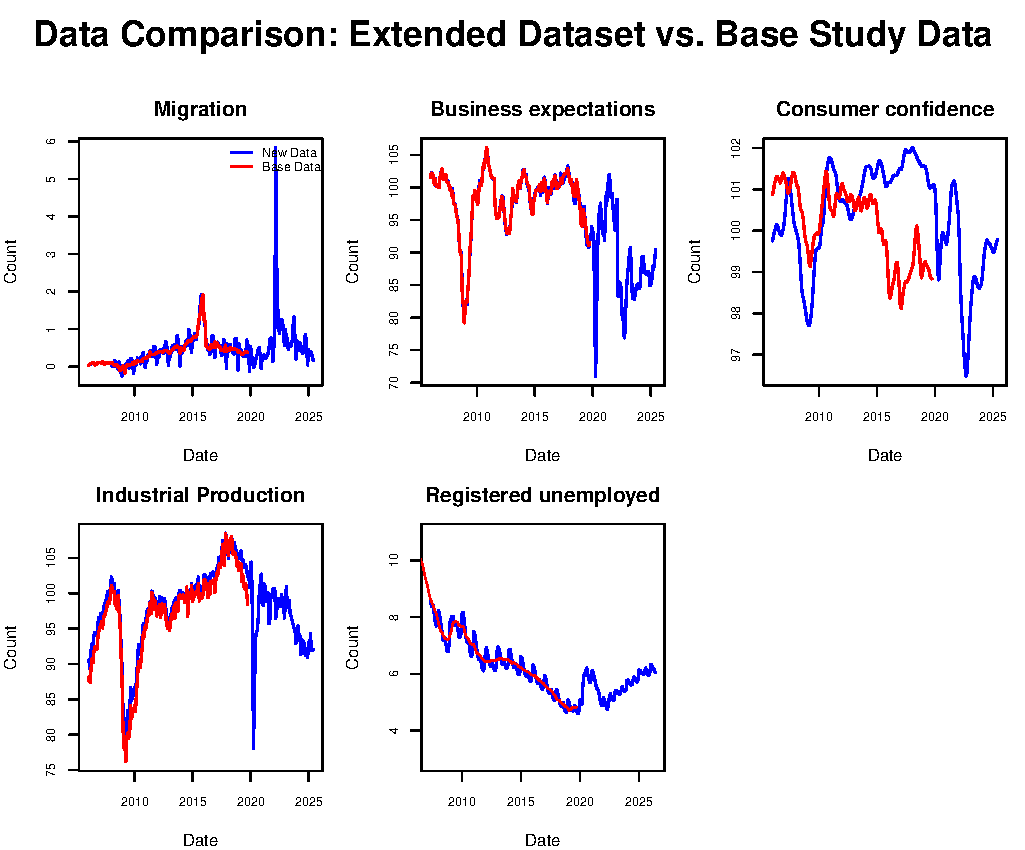
\includegraphics[width=12cm]{./../code/images/NewDataset/From2006To2019/dataComparison.pdf}
    	\caption{Data Comparison: Extended Dataset vs.\ Base Study Data. Five time-series charts (2010--2025) comparing New Data (blue) and Base Data (red) for Migration, Business expectations, Consumer confidence, Industrial Production, and Registered unemployed.}
    	\label{data_comparison}
    \end{figure}
    
    \subsection{Identification}
    \label{identification}
    
    We identify immigration and sentiment shocks with a recursive (Cholesky) ordering, following \parencite{maffei2021does} for the migration block and extending it by placing our new Bundestag immigration sentiment measure last, as in Eq.~\ref{eq:alt_variables}. We report three specifications, one per sentiment measure ($i \in \{\mathit{Government}, \mathit{Opposition}\}$); only the sentiment series changes across them, so the migration and macro block ordering stays fixed, and any difference in results can be attributed to the sentiment measure itself, not the identification scheme.
    
    \paragraph{Ordering the migration variable.} Arrivals are ordered first, assuming German economic conditions do not affect migration within the same month: as \parencite{maffei2021does} argue, deciding to migrate, getting authorization, and arriving takes longer than a month, so a same-month economic shock is unlikely to drive contemporaneous migration.
    
    \paragraph{Ordering the macroeconomic block.} We order $\text{BExp}_t, \text{CConf}_t, \text{IndPr}_t, \text{UnemplR}_t$, following \parencite{maffei2021does}: the forward-looking survey measures (expectations, confidence) come before the realized ("harder") indicators (production, unemployment). This internal ordering is not critical to our results, since both survey and realized variables sit between arrivals and sentiment in every specification; reordering within this block does not affect the sentiment ordering or the identification of the sentiment shock, our main object of interest. We test sensitivity to this choice in Section~\ref{sec:robustness}.
    
    \paragraph{Ordering the sentiment variable.} Sentiment is ordered last because parliamentary immigration rhetoric is likely to respond contemporaneously to prevailing economic and social conditions, while its effects on migration and macroeconomic outcomes are expected to operate with a delay through public discourse and social amplification \parencite{abdelatif2026uncertainty,rakers20232015}. The recursive identification therefore assumes that macroeconomic and migration variables may affect sentiment within the month, but sentiment does not affect them contemporaneously. This is an identifying assumption, which we assess through alternative recursive orderings in Section~\ref{sec:robustness}.
    
    
    \paragraph{Predicted signs.} This ordering implies directional predictions we can check against our results. If sentiment genuinely carries information about future immigration and economic conditions, a one-standard-deviation rise in immigration sentiment should, over the following one to two years: (i) raise arrivals, business expectations, and industrial production; (ii) lower consumer confidence in the short run, consistent with natives reading more open rhetoric as a signal of stronger labour-market competition; and (iii) lower unemployment over the medium term. Table~\ref{tab:predicted_signs} summarizes these predictions.
    \begin{table}[h]
    	\centering
    	\small
    	\begin{tabular}{lcc}
    		\hline
    		Variable & Sentiment shock \\
    		\hline
    		Arrivals & $+$\\
    		Business expectations & $+$ \\
    		Consumer confidence & $-$ (short run) \\
    		Industrial production & $+$ \\
    		Unemployment & $-$ (medium run) \\
    		\hline
    	\end{tabular}
    	\caption{\small Predicted sign of the response to a one-standard-deviation sentiment shock, under the identifying assumptions in this section.}
    	\label{tab:predicted_signs}
    \end{table}
    
    \subsection{Results}
    
    This section presents the estimation results for several Bayesian VAR
    specifications, using different datasets and sample periods, and interprets
    the findings in light of the existing literature. We proceed in three steps.
    First, we replicate the baseline results of \parencite{maffei2021does} using
    their original dataset and extend their model with three measures of
    immigration-related political sentiment (government, opposition, Bundestag). Second, we re-estimate the same specifications on a reconstructed
    dataset covering an extended sample period through June 2025. Third, we
    summarize what is robust across specifications and datasets and what is not.
    
    \subsubsection{Original Dataset from \parencite{maffei2021does}}
 
    \begin{figure}[h]
    	\begin{center}
    		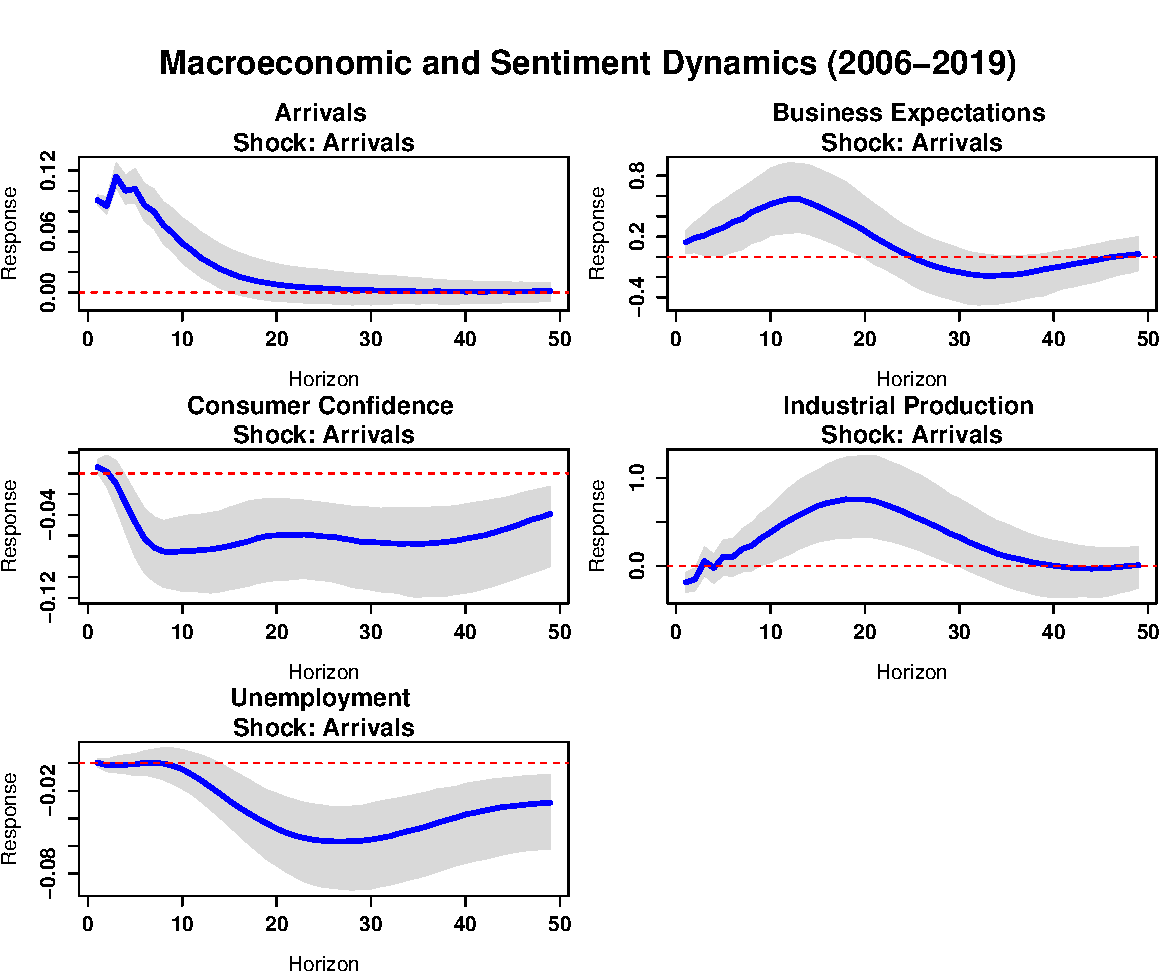
\includegraphics[width=14cm]{./../code/images/From2006To2019/originalStudyResult.pdf}
    		\caption{\small\textbf{Impulse response functions to a one-standard-deviation net migration shock.} 
    			The plots present the first main result of \parencite{maffei2021does}, showing the responses of the endogenous variables to a positive shock to net migration. 
    			The impulse responses are obtained from a recursively identified Bayesian VAR model with three lags and Normal--Wishart priors. 
    			The shaded areas represent the 68\% credible intervals based on posterior draws.}
    		\label{org_irf_study}
    	\end{center}
    \end{figure}
    
    We first reproduce the main results of \parencite{maffei2021does} using their
    original dataset. Our results are broadly consistent with theirs
    (Figure~\ref{org_irf_study}). A positive shock to immigration leads to a
    short-term increase in business expectations and industrial production, while
    consumer confidence declines significantly. The original authors interpret
    this decline as reflecting concerns among the German population about
    increased labour-market competition; we return to this interpretation, and
    its limits, below. Unemployment also decreases following the immigration
    shock, with the response becoming significant approximately nine months after
    impact.
    
   \paragraph{Extending the baseline model with sentiment measures.}
   
   Figures~\ref{fig:govt_sentiment_irf}, \ref{fig:opp_sentiment_irf}, and \ref{fig:bundestag_sentiment_irf} show the responses of the endogenous variables to a positive shock in immigration sentiment, as reflected in speeches by government members, opposition members, and the Bundestag as a whole, respectively.
   
   Across all three shocks, business expectations and industrial production decline significantly over comparable horizons. Unemployment rises significantly following opposition and Bundestag sentiment shocks (see  \ref{fig:opp_sentiment_irf}, \ref{fig:bundestag_sentiment_irf}), while the response to a government sentiment shock is comparatively weaker (see \ref{fig:govt_sentiment_irf}). Consumer confidence declines significantly only after Bundestag and government sentiment shocks (see \ref{fig:govt_sentiment_irf}, \ref{fig:bundestag_sentiment_irf}); under an opposition sentiment shock, its response remains close to zero. Arrivals decline slightly following all three shocks, but the response is statistically negligible throughout.
   
   \begin{figure}[h]
   	\begin{center}
   		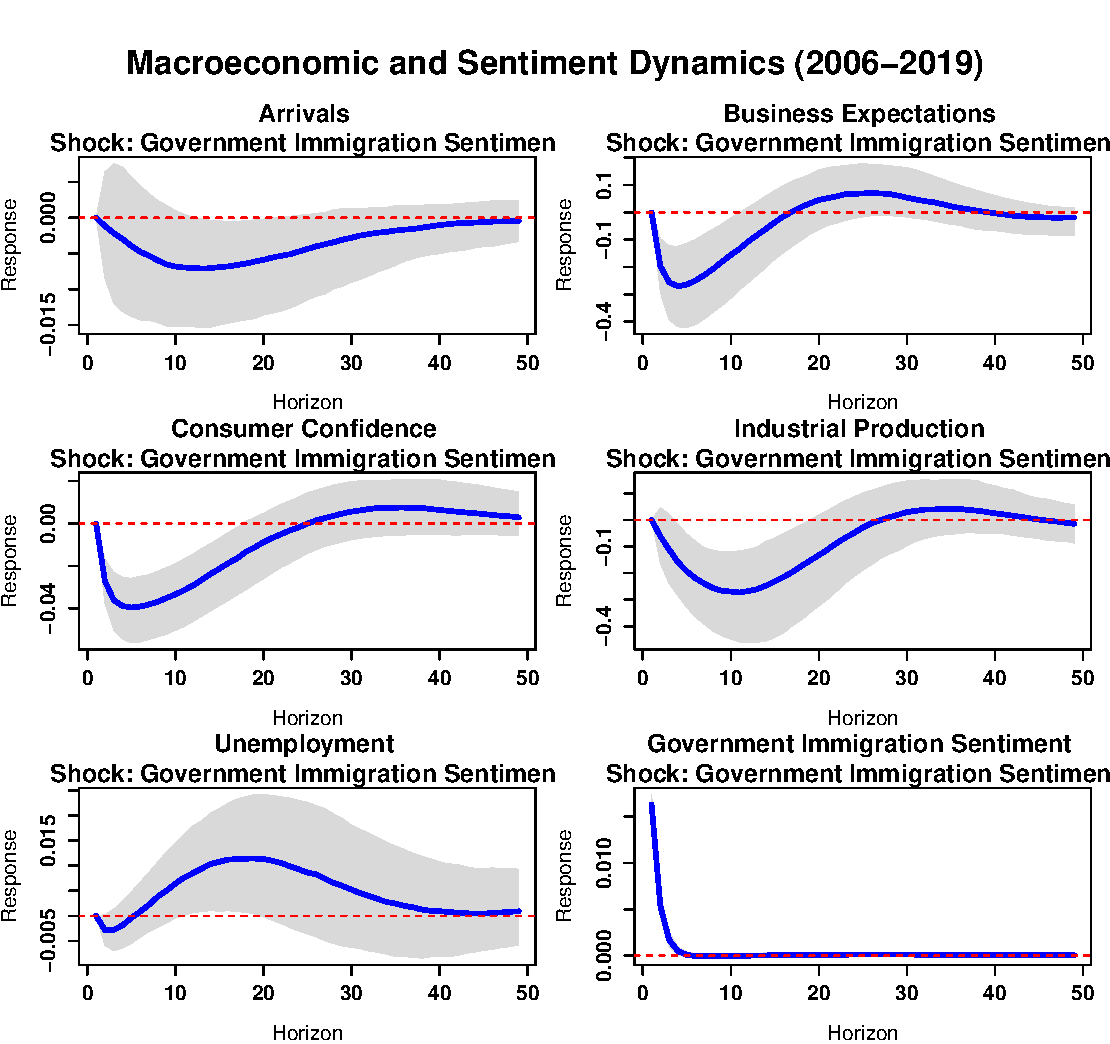
\includegraphics[width=12cm]{./../code/images/From2006To2019/GvtSentimentIrf.pdf}
   		\caption{\small Macroeconomic and Sentiment Dynamics (2006--2019). The figure shows the responses of the endogenous variables to an increase in immigration sentiment, as reflected in speeches by members of the governing parties (horizons 0--50). Shaded areas denote 68\% credible intervals. All impulse responses are obtained from a recursively identified Bayesian VAR model with one lag and Normal--Wishart priors.}
   		\label{fig:govt_sentiment_irf}
   	\end{center}
   \end{figure}
   
   \begin{figure}[h]
   	\begin{center}
   		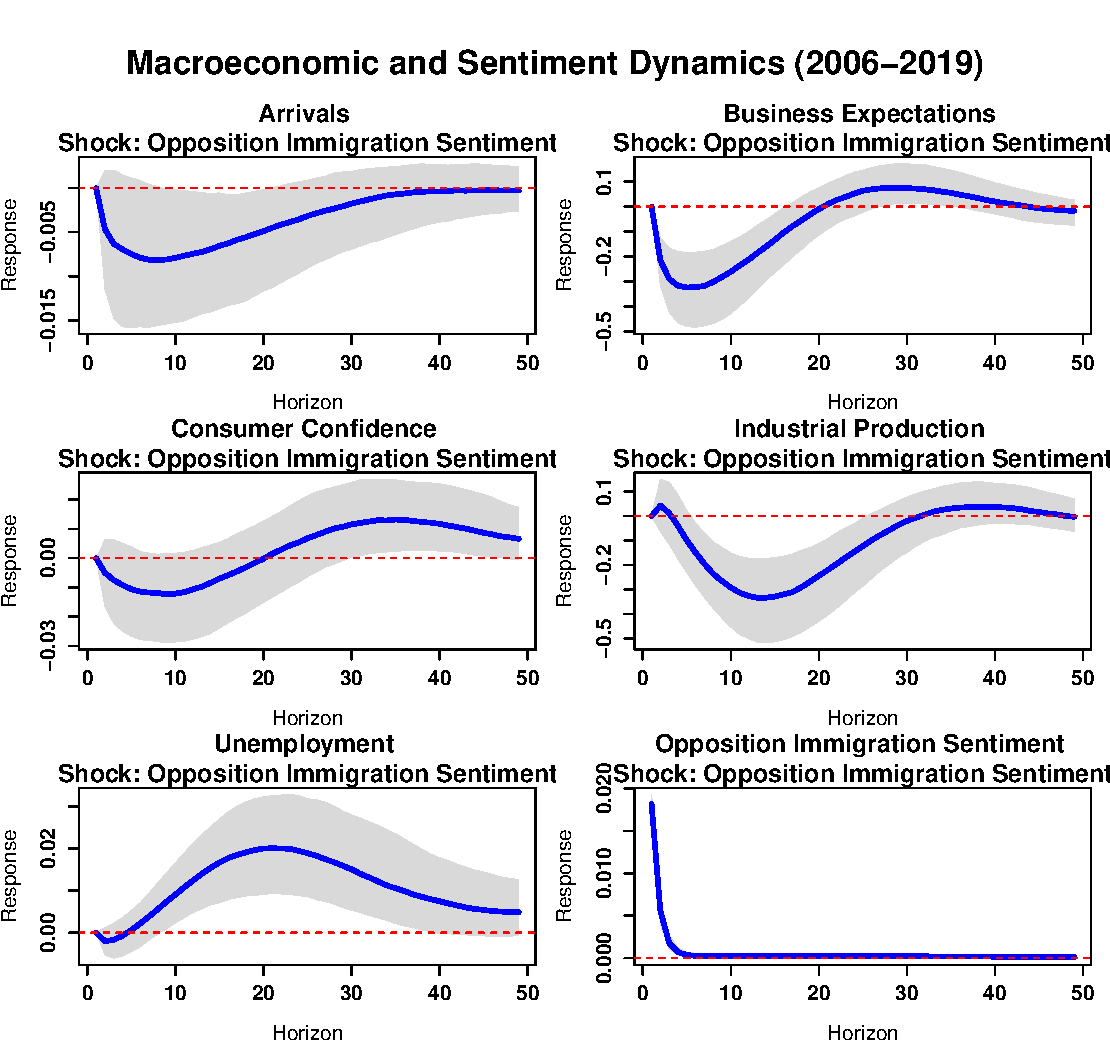
\includegraphics[width=12cm]{./../code/images/From2006To2019/OppSentimentIrf.pdf}
   		\caption{\small Macroeconomic and Sentiment Dynamics (2006--2019). The figure shows the responses of the endogenous variables to an increase in immigration sentiment, as reflected in speeches by members of the opposition parties (horizons 0--50). Shaded areas denote 68\% credible intervals. All impulse responses are obtained from a recursively identified Bayesian VAR model with one lag and Normal--Wishart priors.}
   		\label{fig:opp_sentiment_irf}
   	\end{center}
   \end{figure}
   
   \begin{figure}[h]
   	\begin{center}
   		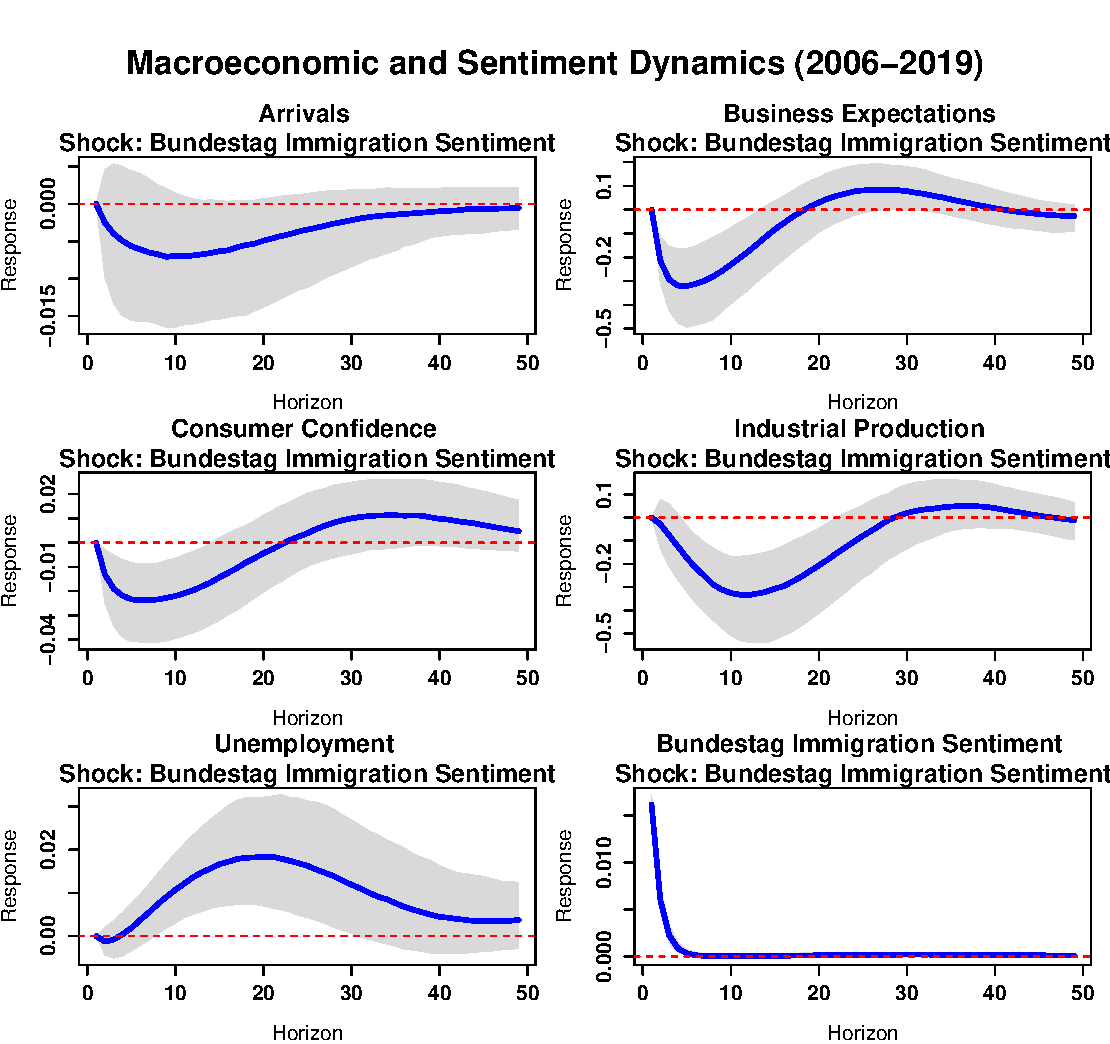
\includegraphics[width=12cm]{./../code/images/From2006To2019/BunSentimentIrf.pdf}
   		\caption{\small Macroeconomic and Sentiment Dynamics (2006--2019). The figure shows the responses of the endogenous variables to an increase in immigration sentiment, as reflected in speeches of all members of the Bundestag (horizons 0--50). Shaded areas denote 68\% credible intervals. All impulse responses are obtained from a recursively identified Bayesian VAR model with one lag and Normal--Wishart priors.}
   		\label{fig:bundestag_sentiment_irf}
   	\end{center}
   \end{figure}
   
   \clearpage
    
    \subsubsection{Extension of the Maffei et al.\ (2021) Dataset to June 2025}
    \label{sec:extended_results}
    
    We now turn to the reconstructed dataset, which extends the sample period
    to June 2025. As discussed above, the reconstructed consumer confidence
    series differs from the one used in the original study (see
    Figure~\ref{data_comparison}), motivating separate estimation over the
    pre-pandemic window 2007--2019 and the full extended window 2007--2025,
    with a COVID-19 exogenous dummy included in the latter.
    
    \begin{figure}[h]
    	\begin{center}
    		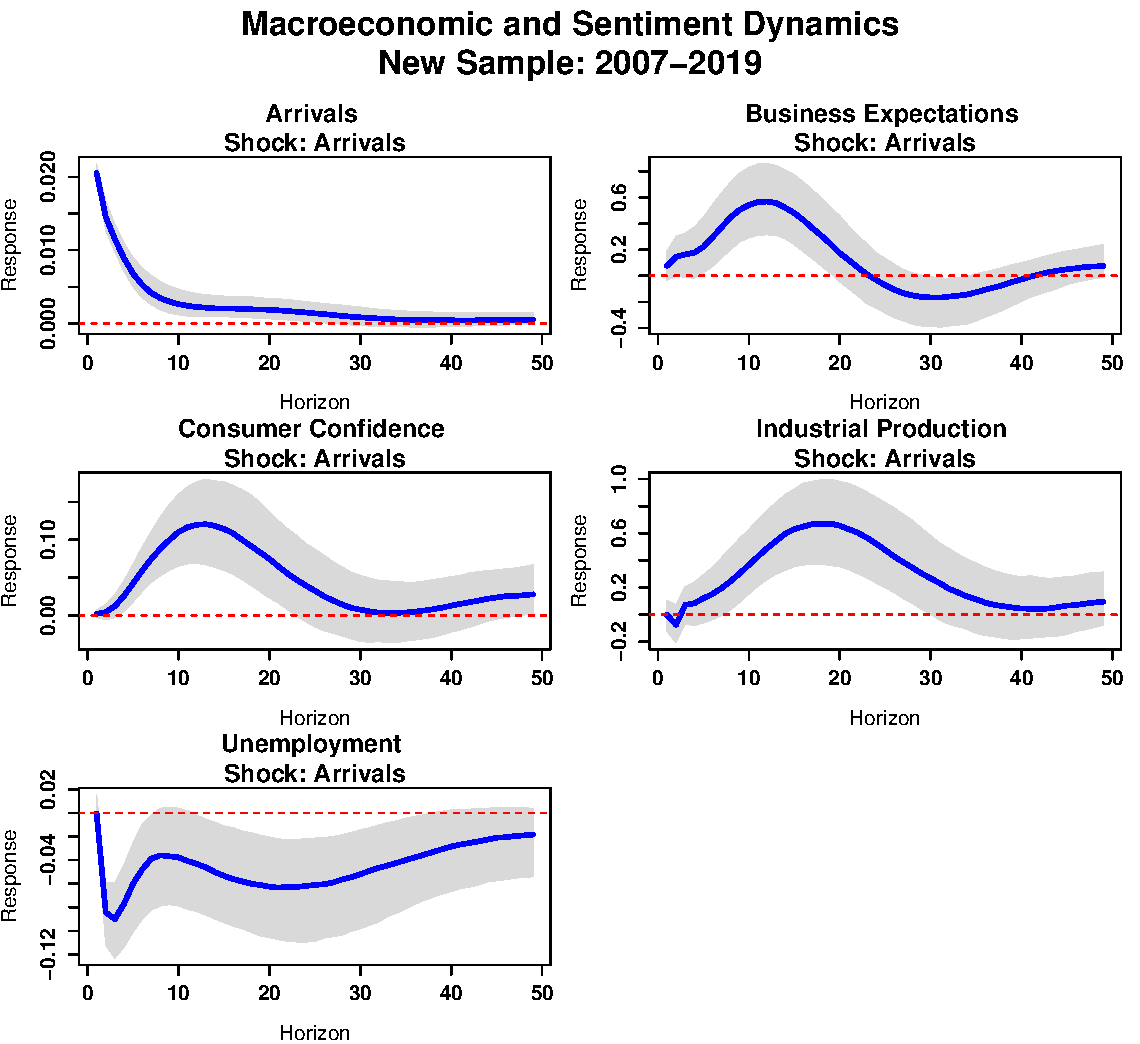
\includegraphics[width=14cm]{./../code/images/NewDataset/From2006To2019/irfOrgVsnewData.pdf}
    		\caption{\small Macroeconomic and Sentiment Dynamics, New Sample: 2007--2019. Impulse response functions to a one-standard-deviation arrival shock. Shaded areas denote 68\% credible intervals. All impulse responses are obtained from a recursively identified Bayesian VAR model with two lags and a diffuse (flat-Jeffreys) prior.}
    		\label{irfOrgVsnewData}
    	\end{center}
    \end{figure}
    
    Figures~\ref{irfOrgVsnewData} and~\ref{irfOrgVsnewData2} report the responses to an arrival shock, partially replicating the findings of the original study (Figure~\ref{org_irf_study}). The decline in unemployment and the rise in industrial production appear across all specifications, though with varying magnitudes. Business expectations and consumer confidence are significant in the original study and the 2007--2019 sample, but lose significance in the extended 2007--2025 sample. Additionally, the reconstructed sample yields a positive consumer confidence response, unlike the negative response in the original study. This difference might stem from two factors: first, discrepancies in the underlying \ac{OECD} consumer confidence data series for the overlapping period; second, the structural multi-crisis environment of 2020--2025 (comprising the pandemic, energy crisis, inflation, and economic stagnation) which alters macroeconomic dynamics.
    
    \begin{figure}[h]
    	\begin{center}
    		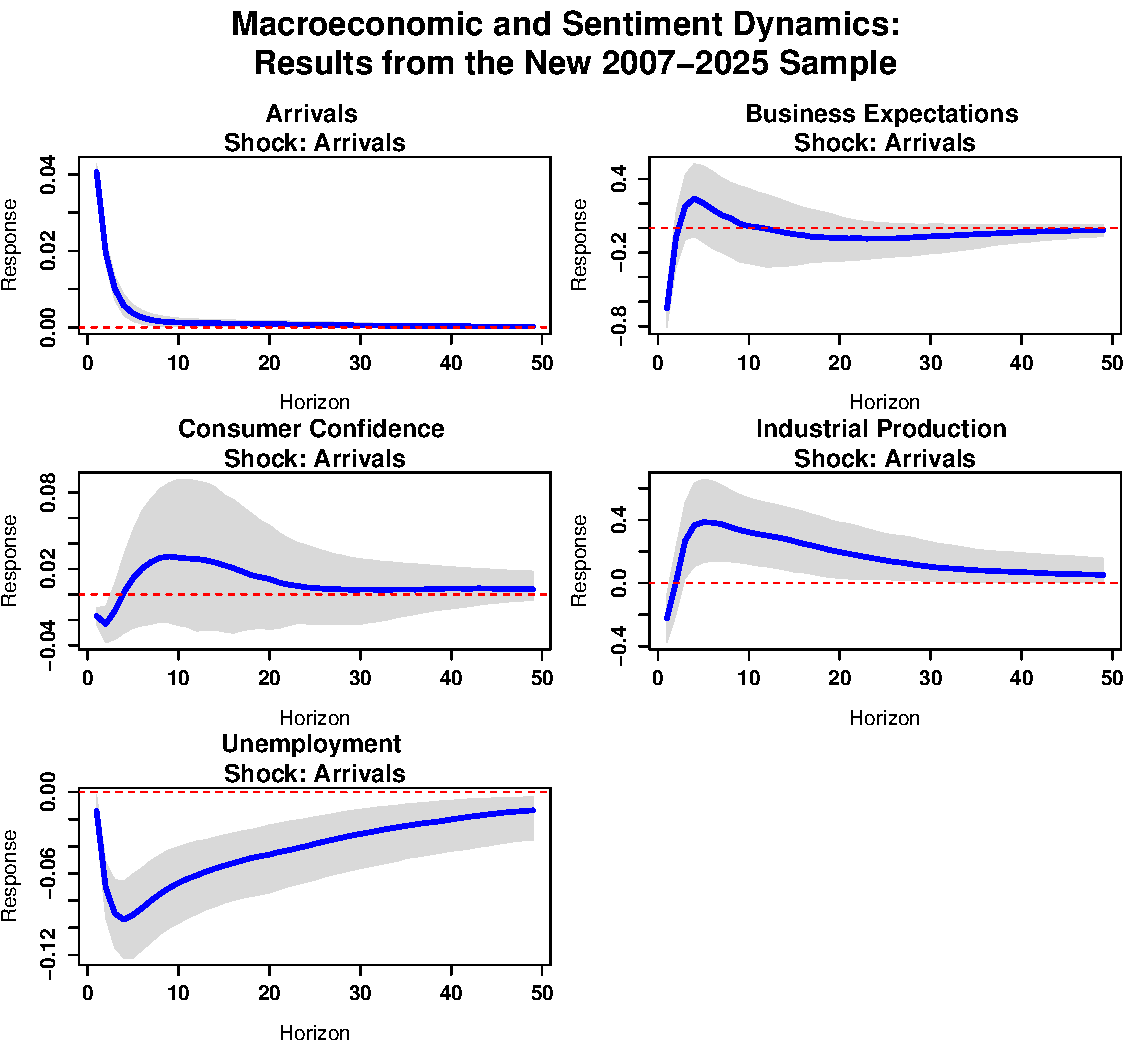
\includegraphics[width=14cm]{./../code/images/NewDataset/From2007To2025/irfOrgVsnewData2.pdf}
    		\caption{\small Macroeconomic and Sentiment Dynamics, New Sample: 2007--2025. Impulse response functions to a one-standard-deviation arrival shock. Shaded areas denote 68\% credible intervals. All impulse responses are obtained from a recursively identified Bayesian VAR model with two lags and a diffuse (flat-Jeffreys) prior, including a COVID-19 exogenous control dummy for observations between March 2020 and October 2021.}
    		\label{irfOrgVsnewData2}
    	\end{center}
    \end{figure}
    
    In short, the reconstructed dataset yields a significant relationship
    between immigration shocks and macroeconomic variables, although the
    strength and significance of this relationship depend on the sample period
    considered. This sensitivity is likely attributable, at least in part, to
    the dataset reconstruction differences discussed in
    Figure~\ref{data_comparison}.
    
    \paragraph{Reconstructed dataset, 2007--2019 window.}
    
    Figures~\ref{fig:gvt_2007_2019_irf}, \ref{fig:opp_2007_2019_irf}, and \ref{fig:bun_2007_2019_irf} show the responses of the endogenous variables to sentiment shocks computed from speeches by government members, opposition members, and the Bundestag as a whole, respectively. The overall pattern is broadly consistent with the original sample (Figures~\ref{fig:govt_sentiment_irf}--\ref{fig:bundestag_sentiment_irf}): business expectations and consumer confidence decline sharply following each shock. The rise in unemployment, however, is markedly stronger and more persistent here than in the original sample (see figures~\ref{fig:govt_sentiment_irf}, \ref{fig:opp_sentiment_irf}, \ref{fig:bundestag_sentiment_irf}), and this is especially pronounced under the opposition and Bundestag sentiment shocks (see figure \ref{fig:opp_2007_2019_irf} ), where the response is both larger in magnitude and slower to revert than under the government shock.
    
    Arrivals respond negatively and significantly to an opposition sentiment shock, while the response is comparatively small and less clearly significant for the government and Bundestag shocks (see figures \ref{fig:gvt_2007_2019_irf}, \ref{fig:bun_2007_2019_irf}). 
    
    \begin{figure}[h]
    	\begin{center}
    		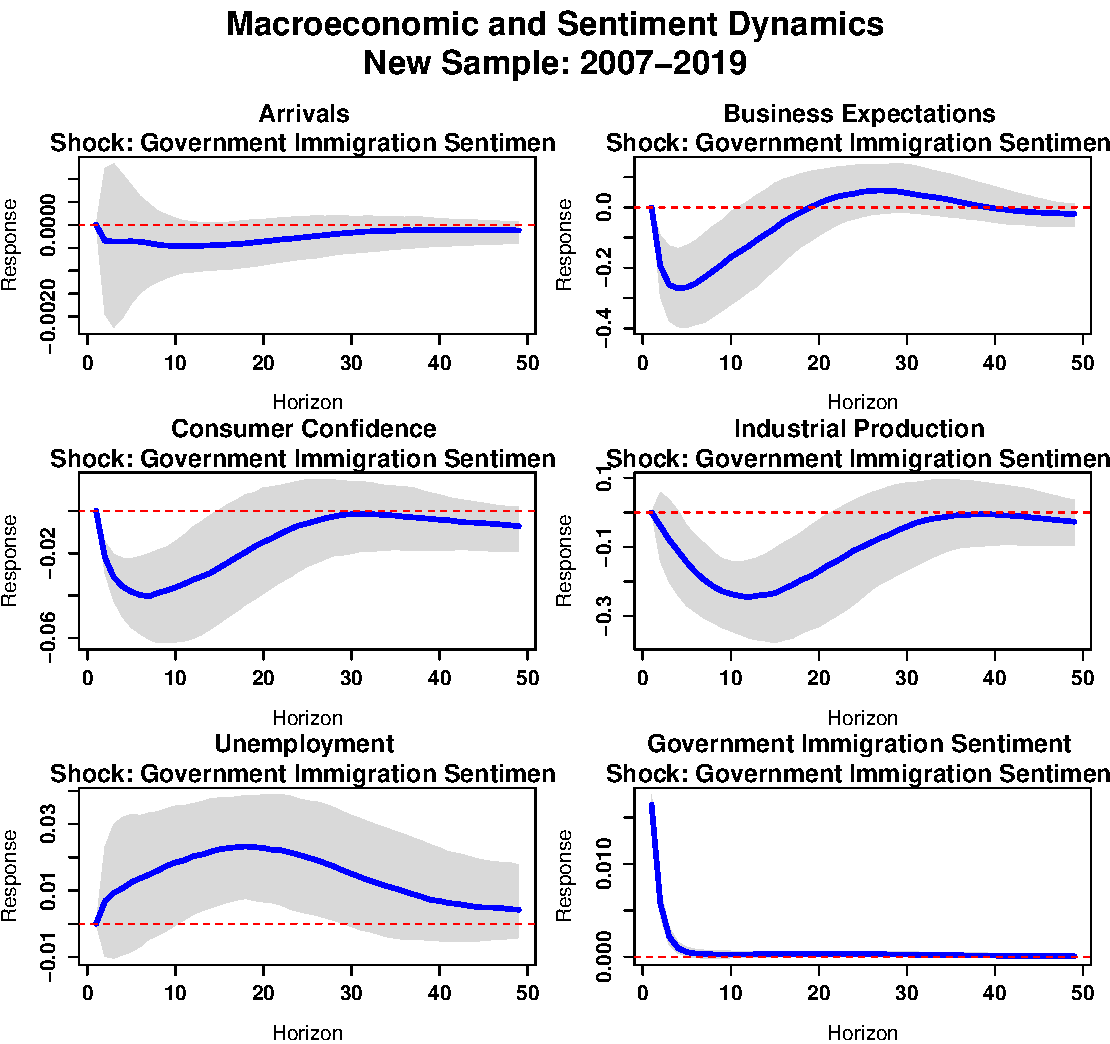
\includegraphics[width=12cm]{./../code/images/NewDataset/From2006To2019/Gvt2007To2019Irf.pdf}
    		\caption{\small Macroeconomic and Sentiment Dynamics, New Sample: 2007--2019. The figure shows the responses of the endogenous variables to an increase in immigration sentiment, as reflected in speeches by members of the governing parties (horizons 0--50). Shaded areas denote 68\% credible intervals. All impulse responses are obtained from a recursively identified Bayesian VAR model with one lag and Normal--Wishart priors.}
    		\label{fig:gvt_2007_2019_irf}
    	\end{center}
    \end{figure}
    
    \begin{figure}[h]
    	\begin{center}
    		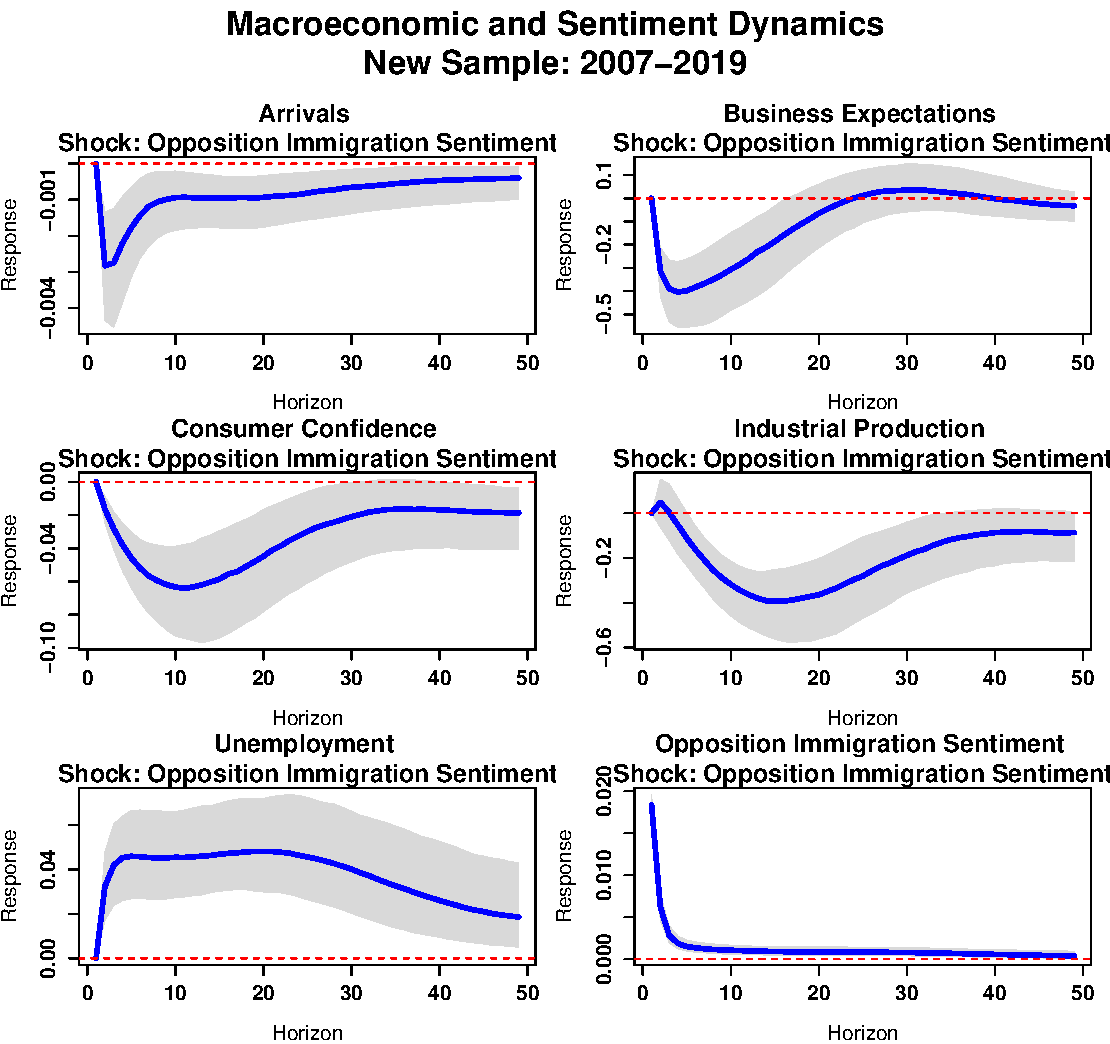
\includegraphics[width=12cm]{./../code/images/NewDataset/From2006To2019/Opp2007To2019Irf.pdf}
    		\caption{\small Macroeconomic and Sentiment Dynamics, New Sample: 2007--2019. The figure shows the responses of the endogenous variables to an increase in immigration sentiment, as reflected in speeches by members of the opposition parties (horizons 0--50). Shaded areas denote 68\% credible intervals. All impulse responses are obtained from a recursively identified Bayesian VAR model with one lag and Normal--Wishart priors.}
    		\label{fig:opp_2007_2019_irf}
    	\end{center}
    \end{figure}
    
    \begin{figure}[h]
    	\begin{center}
    		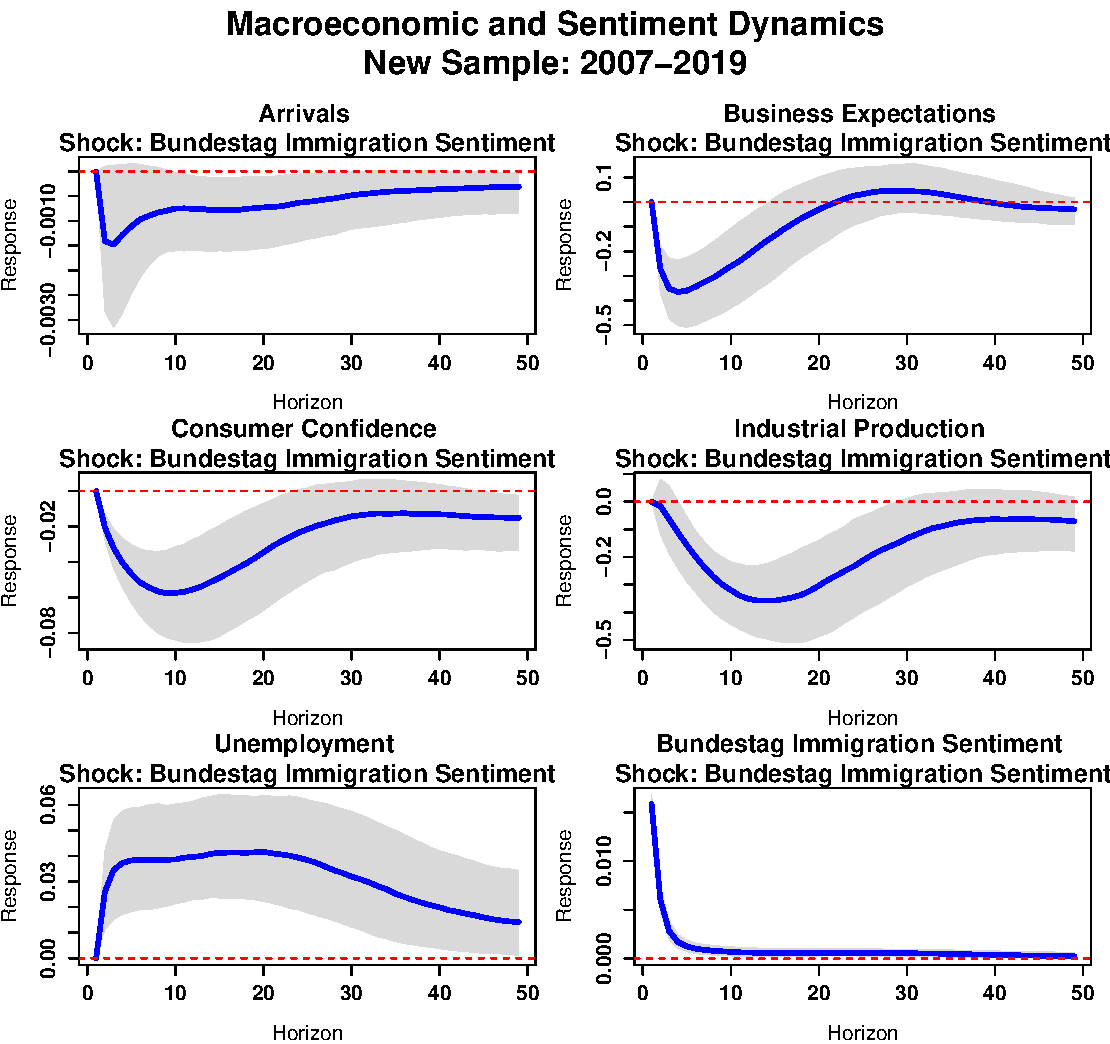
\includegraphics[width=12cm]{./../code/images/NewDataset/From2006To2019/Bu2007To2019Irf.pdf}
    		\caption{\small Macroeconomic and Sentiment Dynamics, New Sample: 2007--2019. The figure shows the responses of the endogenous variables to an increase in immigration sentiment, as reflected in speeches of all members of the Bundestag (horizons 0--50). Shaded areas denote 68\% credible intervals. All impulse responses are obtained from a recursively identified Bayesian VAR model with one lag and Normal--Wishart priors.}
    		\label{fig:bun_2007_2019_irf}
    	\end{center}
    \end{figure}
    
    \clearpage
    
    \paragraph{Extended sample: 2007--2025.}
    
    Figures~\ref{fig:gvt_2007_2025_irf}, \ref{fig:opp_2007_2025_irf}, and \ref{fig:bu_2007_2025_irf} report the corresponding impulse responses. The pattern differs markedly from the government shock, on one hand, and the opposition and Bundestag shocks, on the other. Following a government sentiment shock, most endogenous variables respond weakly and without clear significance (see figure \ref{fig:gvt_2007_2025_irf}), with the exception of unemployment, which remains positive throughout the horizon. Following opposition and Bundestag sentiment shocks, unemployment, business expectations, and consumer confidence all rise significantly, while arrivals decline significantly; industrial production, by contrast, shows no statistically discernible response (see figures~\ref{fig:opp_2007_2025_irf}, \ref{fig:bu_2007_2025_irf}).
    
    \begin{figure}[h]
    	\begin{center}
    		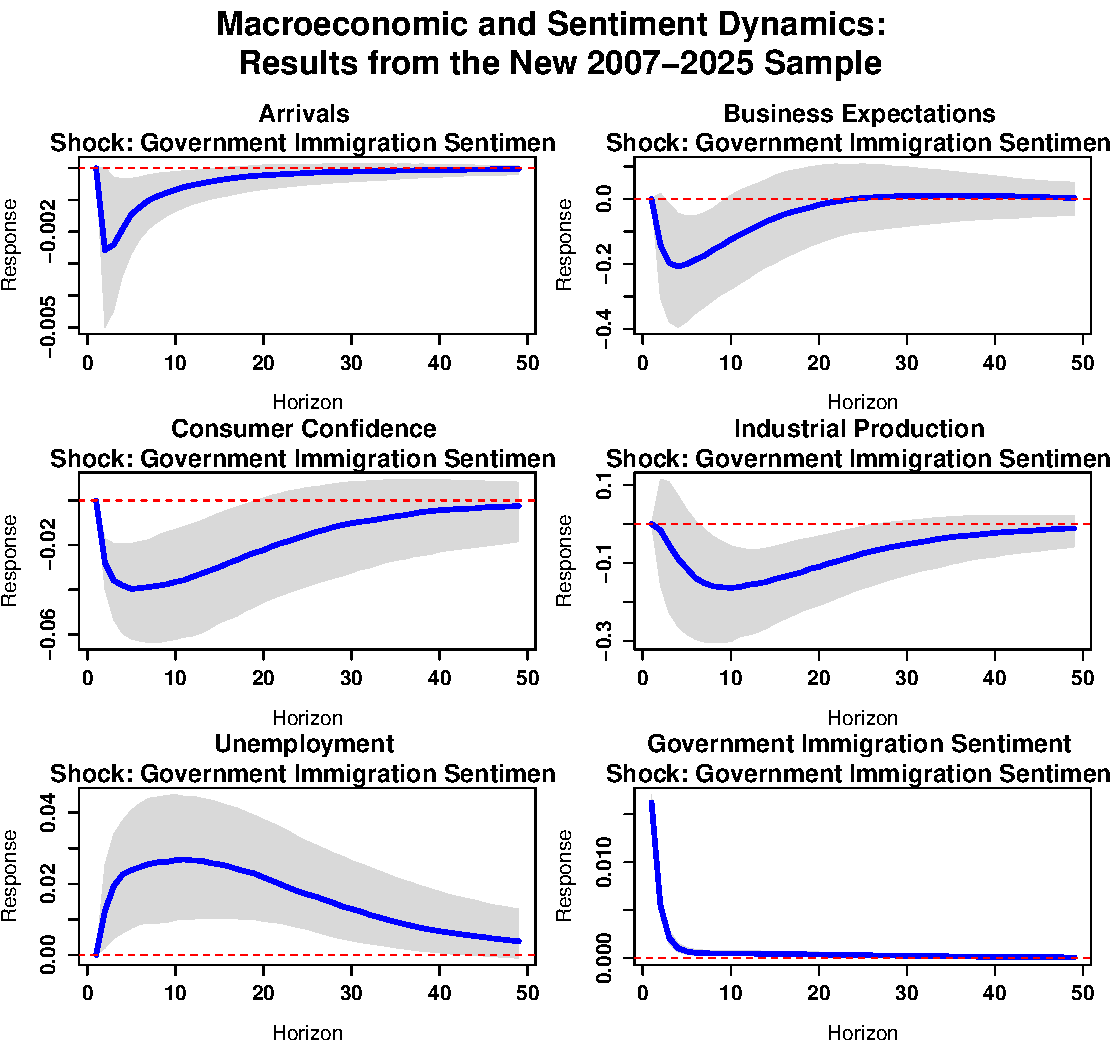
\includegraphics[width=12cm]{./../code/images/NewDataset/From2007To2025/gvtTo2007to2025.pdf}
    		\caption{\small Macroeconomic and Sentiment Dynamics, New Sample: 2007--2025. The figure shows the responses of the endogenous variables to an increase in immigration sentiment, as reflected in speeches by members of the governing parties (horizons 0--50). Shaded areas denote 68\% credible intervals. All impulse responses are obtained from a recursively identified Bayesian VAR model with two lags and Normal--Wishart priors.}
    		\label{fig:gvt_2007_2025_irf}
    	\end{center}
    \end{figure}
    
    \begin{figure}[h]
    	\begin{center}
    		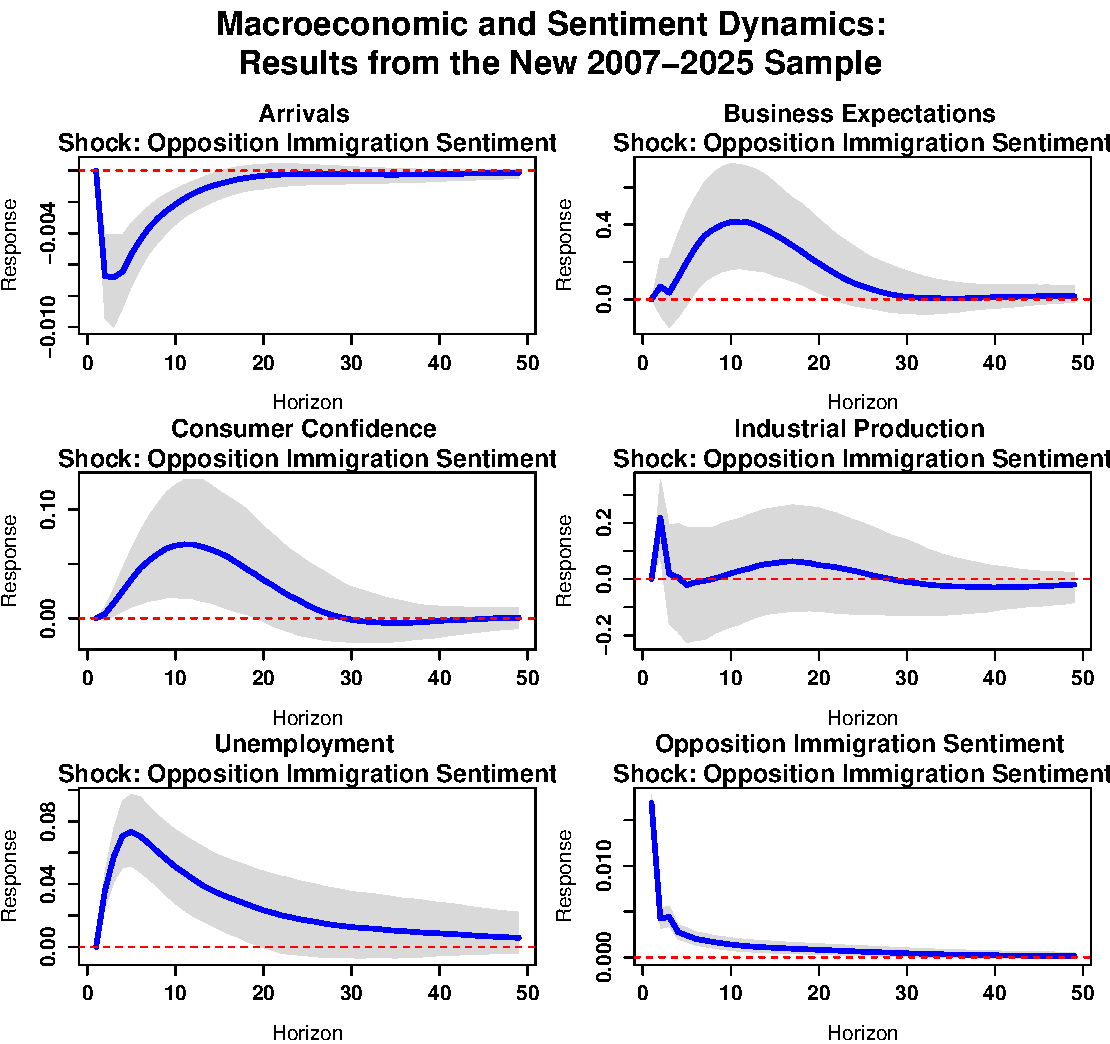
\includegraphics[width=12cm]{./../code/images/NewDataset/From2007To2025/oppto2007to2025.pdf}
    		\caption{\small Macroeconomic and Sentiment Dynamics, New Sample: 2007--2025. The figure shows the responses of the endogenous variables to an increase in immigration sentiment, as reflected in speeches by members of the opposition parties (horizons 0--50). Shaded areas denote 68\% credible intervals. All impulse responses are obtained from a recursively identified Bayesian VAR model with two lags and Normal--Wishart priors.}
    		\label{fig:opp_2007_2025_irf}
    	\end{center}
    \end{figure}
    
    \begin{figure}[h]
    	\begin{center}
    		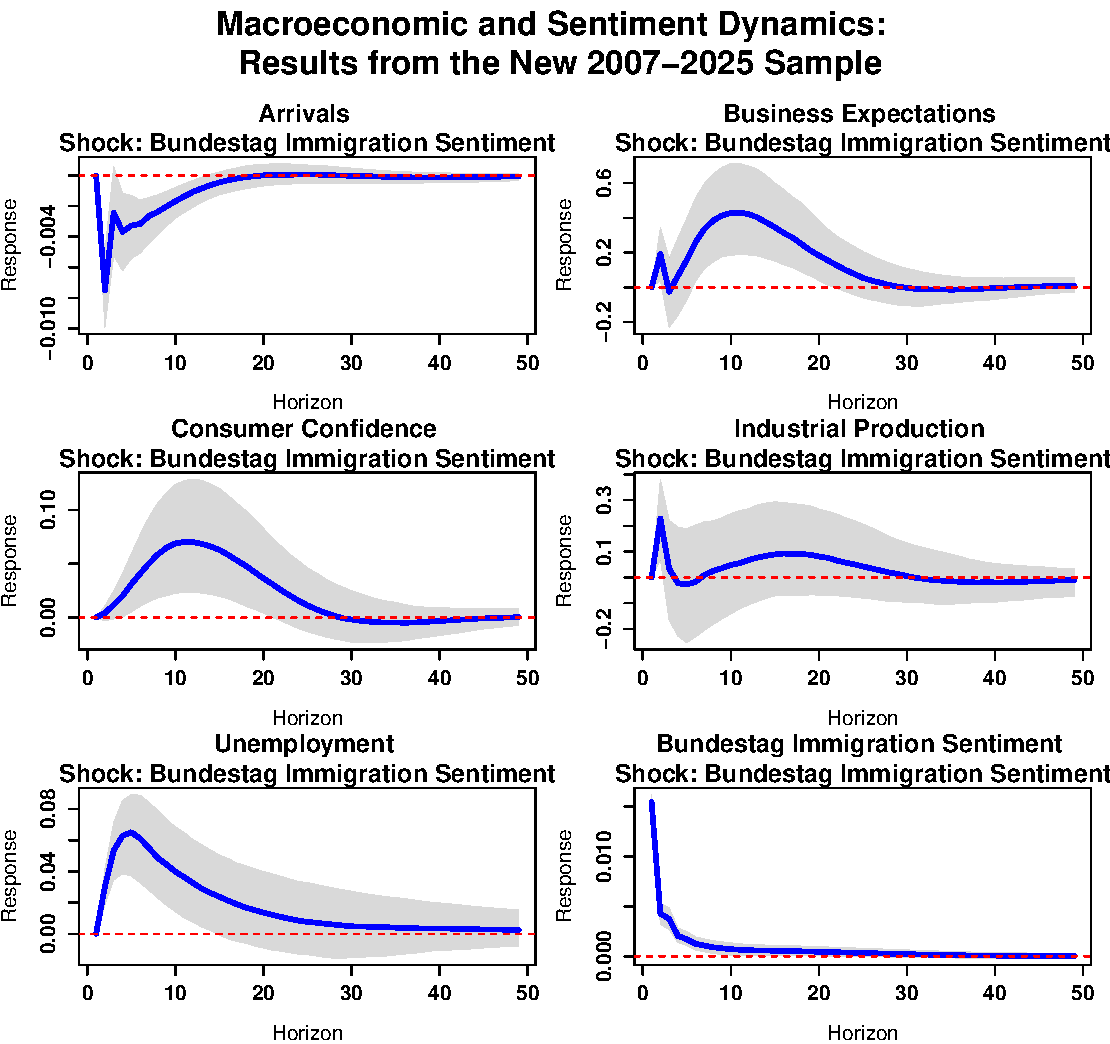
\includegraphics[width=12cm]{./../code/images/NewDataset/From2007To2025/BUto2007to2025.pdf}
    		\caption{\small Macroeconomic and Sentiment Dynamics, New Sample: 2007--2025. The figure shows the responses of the endogenous variables to an increase in immigration sentiment, as reflected in speeches of all members of the Bundestag (horizons 0--50). Shaded areas denote 68\% credible intervals. All impulse responses are obtained from a recursively identified Bayesian VAR model with two lags and Normal--Wishart priors.}
    		\label{fig:bu_2007_2025_irf}
    	\end{center}
    \end{figure}
    
    Taken together, sentiments are associated with subsequent macroeconomic dynamics. However, we defer a detailed economic interpretation of these findings to the robustness section (\ref{sec:robustness}). This postponement is necessary due to limitations identified in our Doc2Vec model—specifically, its sensitivity to negative rhetoric, which can bias the computation of immigration sentiment within Bundestag speeches.
    
    \clearpage
    
    \subsection{Robustness}
    \label{sec:robustness}
    
    As a further robustness check on the identification scheme, we re-estimate
    the opposition-sentiment specification on the pre-crisis subsample
    2007--2014 under three alternative recursive orderings. Restricting the
    sample to this window additionally allows us to assess whether the
    sentiment--unemployment relationship documented in
    Section~\ref{sec:extended_results} is already present before the
    2015--2016 refugee episode, rather than being generated primarily by it.
    
    \paragraph{Specification 1: baseline ordering.} The first ordering follows
    the baseline scheme of Equation~\ref{eq:short_baseline}, with arrivals
    ordered first, the macroeconomic block ordered as business expectations,
    consumer confidence, and industrial production, and opposition sentiment
    ordered last:
    \begin{equation}
    	\mathbf{y}_t =
    	\left[
    	\text{Arrivals}_t,\,
    	\text{BusExp}_t,\,
    	\text{ConsConf}_t,\,
    	\text{IndProd}_t,\,
    	\text{Unemp}_t,\,
    	\text{Sent}^{\mathit{Opp}}_t
    	\right]^{\prime}.
    	\label{eq:short_baseline}
    \end{equation}
    
    Figure~\ref{fig:short1} reports the resulting impulse responses. Arrivals
    decline on impact and remain significant for approximately 7 months
    following the shock, while unemployment rises on impact and remains
    significant for approximately 10--15 months. This indicates that the
    effect of opposition immigration sentiment on arrivals and unemployment is
    already present in the pre-crisis window, although it is comparatively
    short-lived relative to the full 2007--2025 sample.
    
    \paragraph{Specification 2: reordered macroeconomic block.} The second
    ordering places the two realized indicators, industrial production and
    unemployment, ahead of the two survey-based expectations variables, while
    keeping arrivals first and sentiment last:
    \begin{equation}
    	\mathbf{y}_t =
    	\left[
    	\text{Arrivals}_t,\,
    	\text{IndProd}_t,\,
    	\text{Unemp}_t,\,
    	\text{BusExp}_t,\,
    	\text{ConsConf}_t,\,
    	\text{Sent}^{\mathit{Opp}}_t
    	\right]^{\prime}.
    	\label{eq:short_macro}
    \end{equation}
    Figure~\ref{fig:short2} shows results essentially unchanged from
    Specification~1: the responses of arrivals and unemployment remain of
    similar magnitude and significance, indicating that the results are robust
    to this reordering.
    
    \paragraph{Specification 3: sentiment ordered second.} The third ordering
    moves opposition sentiment to the second position, immediately after
    arrivals and ahead of the entire macroeconomic block, thereby allowing
    sentiment to affect all four macroeconomic variables contemporaneously:
    \begin{equation}
    	\mathbf{y}_t =
    	\left[
    	\text{Arrivals}_t,\,
    	\text{Sent}^{\mathit{Opp}}_t,\,
    	\text{IndProd}_t,\,
    	\text{Unemp}_t,\,
    	\text{BusExp}_t,\,
    	\text{ConsConf}_t
    	\right]^{\prime}.
    	\label{eq:short_sent2nd}
    \end{equation}
    
    Figure~\ref{fig:short3} shows a similar pattern to Specifications 1 and 2,
    with arrivals and unemployment again responding significantly and over
    comparable horizons. Overall, the three orderings deliver consistent
    conclusions, suggesting that the documented responses are not highly sensitive to the alternative recursive orderings considered.
    
    \begin{figure}[h]
    	\begin{center}
    		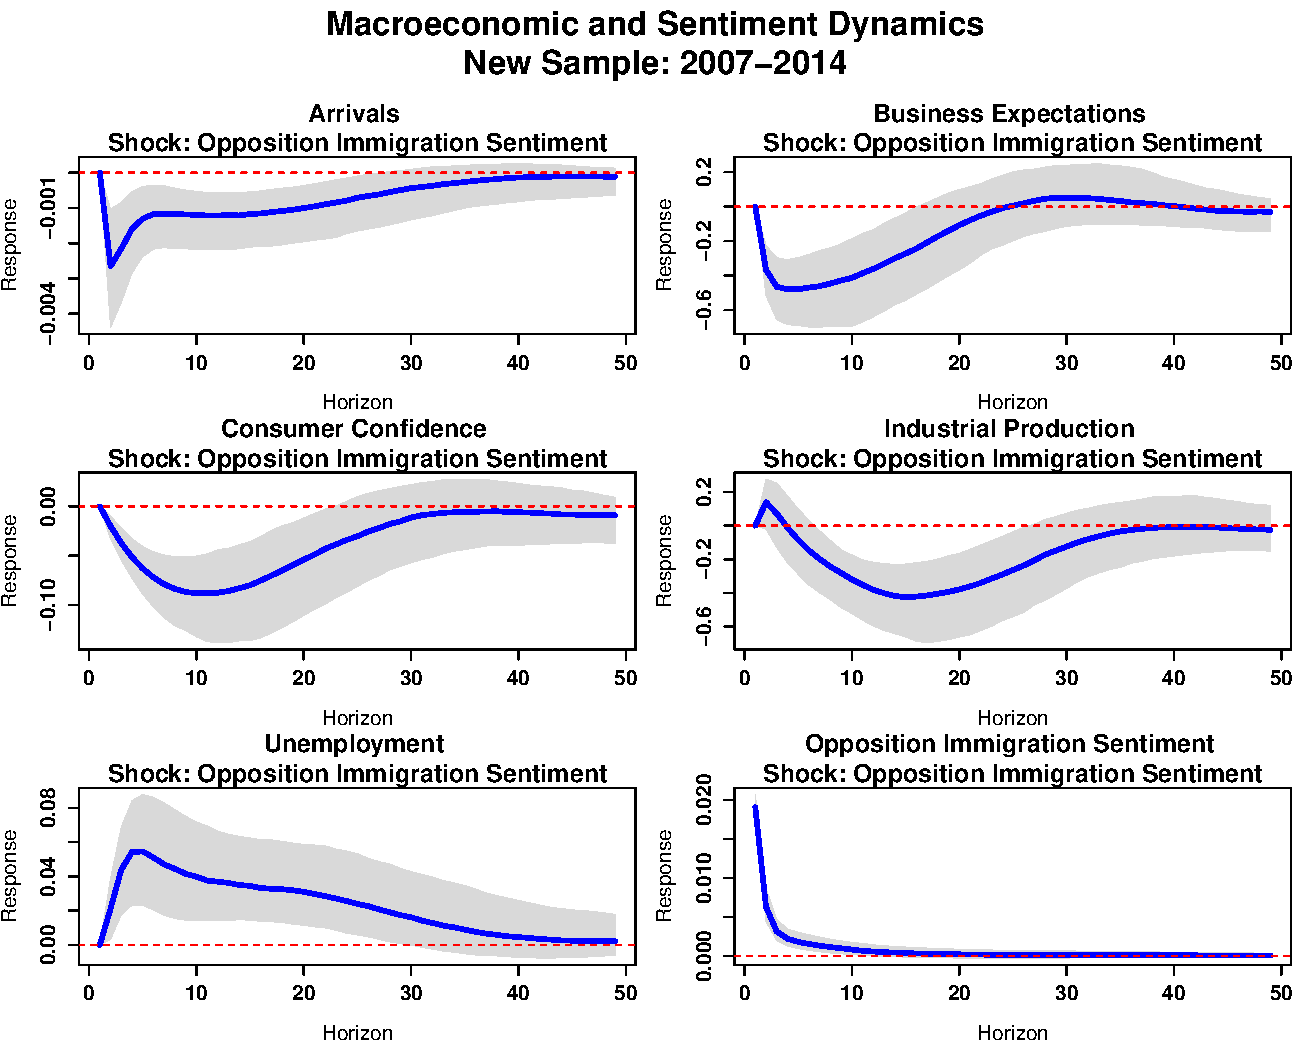
\includegraphics[width=14cm]{./../code/images/robustness/short2007to2014_baseline.pdf}
    		\caption{\small\textbf{Robustness check, Specification 1 (baseline ordering), sample 2007--2014.} The figure shows the responses of the endogenous variables to an increase in immigration sentiment, as reflected in speeches by members of the opposition parties (horizons 0--50). Shaded areas denote 68\% credible intervals. All impulse responses are obtained from a recursively identified Bayesian VAR model with one lag and Normal--Wishart priors.}
    		\label{fig:short1}
    	\end{center}
    \end{figure}
    
    \begin{figure}[h]
    	\begin{center}
    		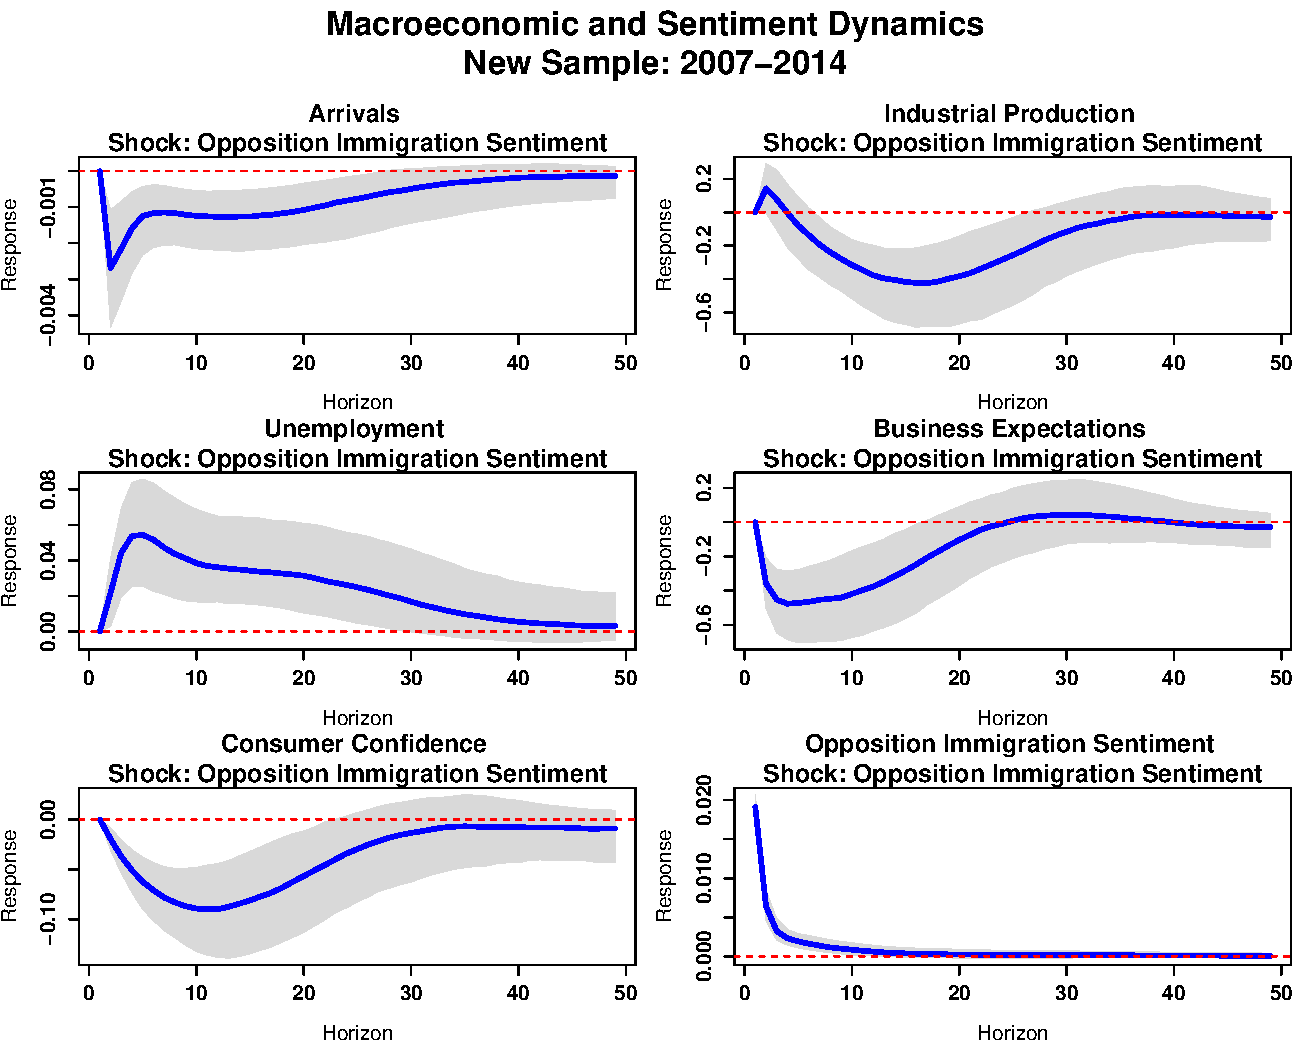
\includegraphics[width=14cm]{./../code/images/robustness/short2007to2014_macroreorder.pdf}
    		\caption{\small\textbf{Robustness check, Specification 2 (reordered macroeconomic block), sample 2007--2014.} The figure shows the responses of the endogenous variables to an increase in immigration sentiment, as reflected in speeches by members of the opposition parties (horizons 0--50). Shaded areas denote 68\% credible intervals. All impulse responses are obtained from a recursively identified Bayesian VAR model with one lag and Normal--Wishart priors.}
    		\label{fig:short2}
    	\end{center}
    \end{figure}
    
    \begin{figure}[h]
    	\begin{center}
    		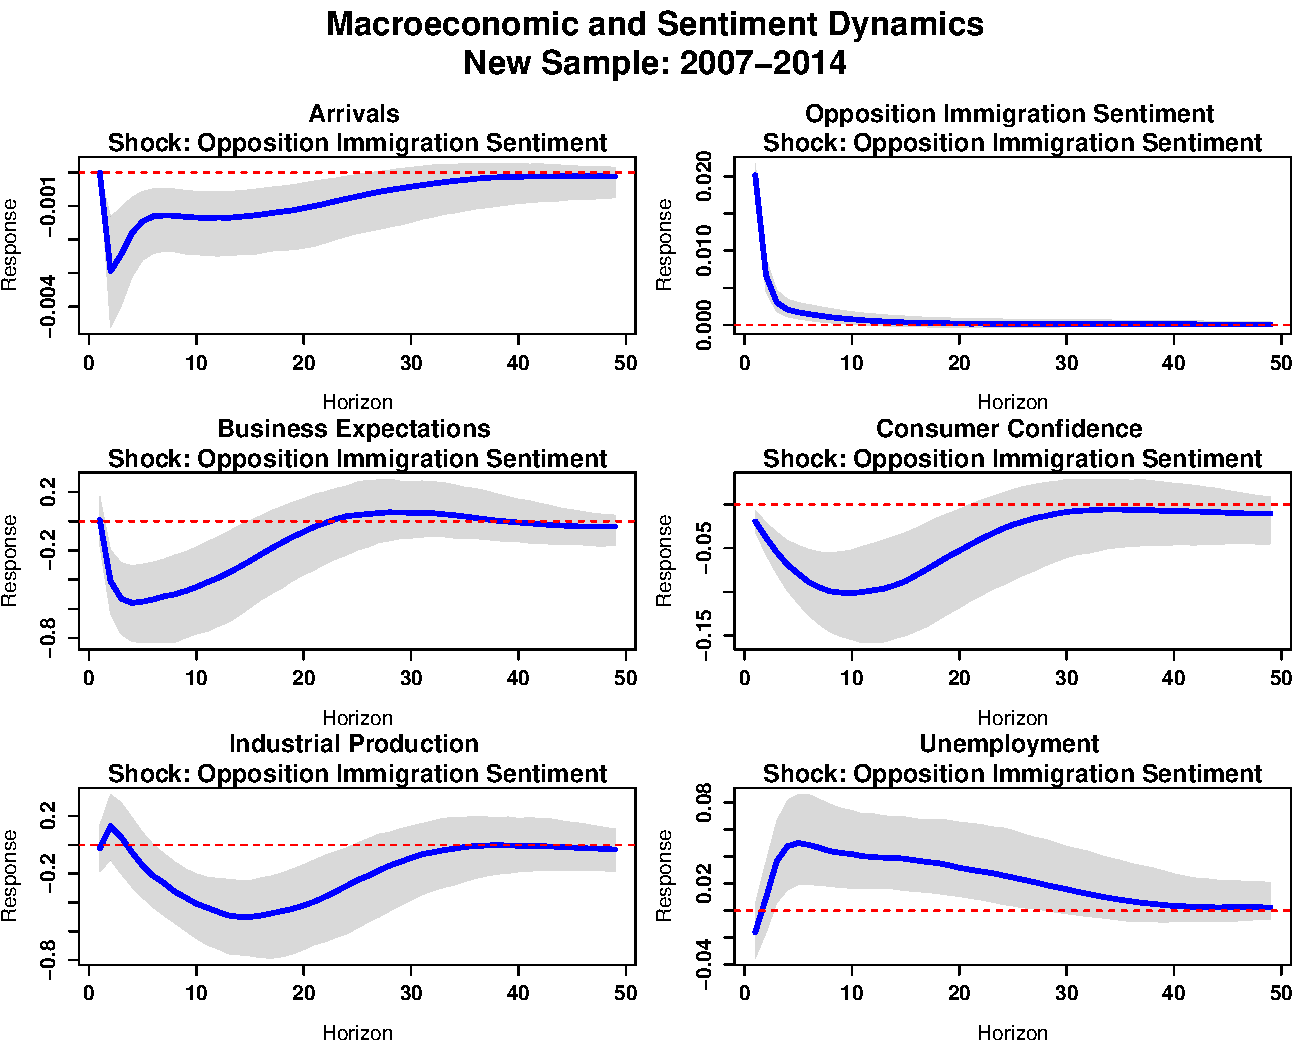
\includegraphics[width=14cm]{./../code/images/robustness/short2007to2014_sentsecond.pdf}
    		\caption{\small\textbf{Robustness check, Specification 3 (sentiment ordered second), sample 2007--2014.} The figure shows the responses of the endogenous variables to an increase in immigration sentiment, as reflected in speeches by members of the opposition parties (horizons 0--50). Shaded areas denote 68\% credible intervals. All impulse responses are obtained from a recursively identified Bayesian VAR model with one lag and Normal--Wishart priors.}
    		\label{fig:short3}
    	\end{center}
    \end{figure}
    
    \begin{figure}[h]
    	\begin{center}
    		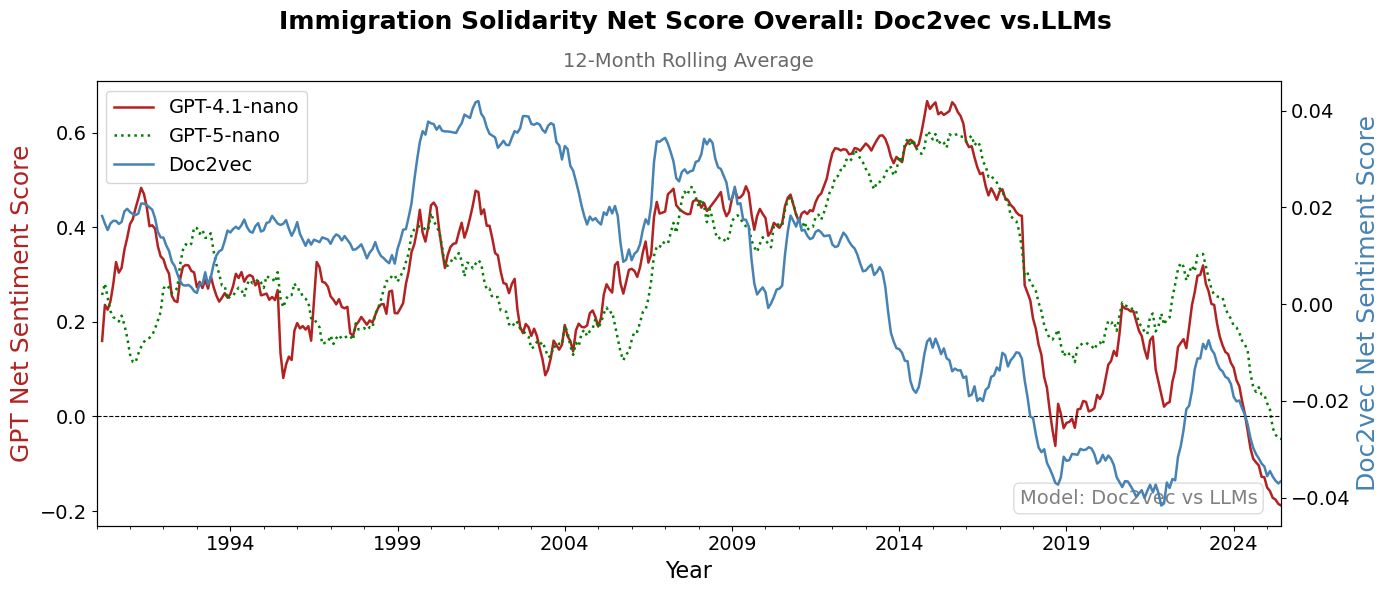
\includegraphics[width=14cm]{./../code/images/robustness/doc2vecandgpt.png}
    		\caption{12-month rolling average of the immigration solidarity net score comparing Doc2vec and \ac{LLM}.}
    		\label{fig:doc2vec_gpt_sentiment}
    	\end{center}
    \end{figure}
    
    
     
    \clearpage
     
     \paragraph{Specification 4: alternative sentiment measure \ac{LLM}.}
     
     The three specifications above test robustness to the recursive ordering, keeping the
     sentiment measure fixed. A separate concern, raised in
     Section~\ref{migration-speech-identification-and-dictionary-construction}, is that
     Doc2Vec struggles with negation. Manual inspection found several misclassified
     speeches, and even after the correction in Section~\ref{sec:party_averages}, average
     sentiment for some parties (CDU/CSU, Bündnis 90/Die Grünen, Die Linke) still looked
     implausible. As a check on the sentiment measure itself, we re-estimate immigration
     sentiment using large language models (GPT-4.1-nano and GPT-5-nano), following
     \textcite{kostikova2024fine}. Each migration-related sentence is classified into
     solidarity or anti-solidarity subtypes, and we build a monthly net-solidarity score
     the same way as the dictionary-based measure, separately for government and
     opposition speakers. The full prompt is in Appendix~\ref{app:gpt_prompt}.
     
     Figures~\ref{fig:gpt_party_average}, \ref{fig:gpt_compassion_party}, and
     \ref{fig:gpt_economic_party} show that the LLM-based measure ranks parties in a way
     that better matches their known public rhetoric than the uncorrected dictionary
     measure. This supports our earlier suspicion that some of the discrepancies in
     Section~\ref{sec:party_averages} came from negation-related misclassification.
     
     \begin{figure}[h]
     	\begin{center}
     		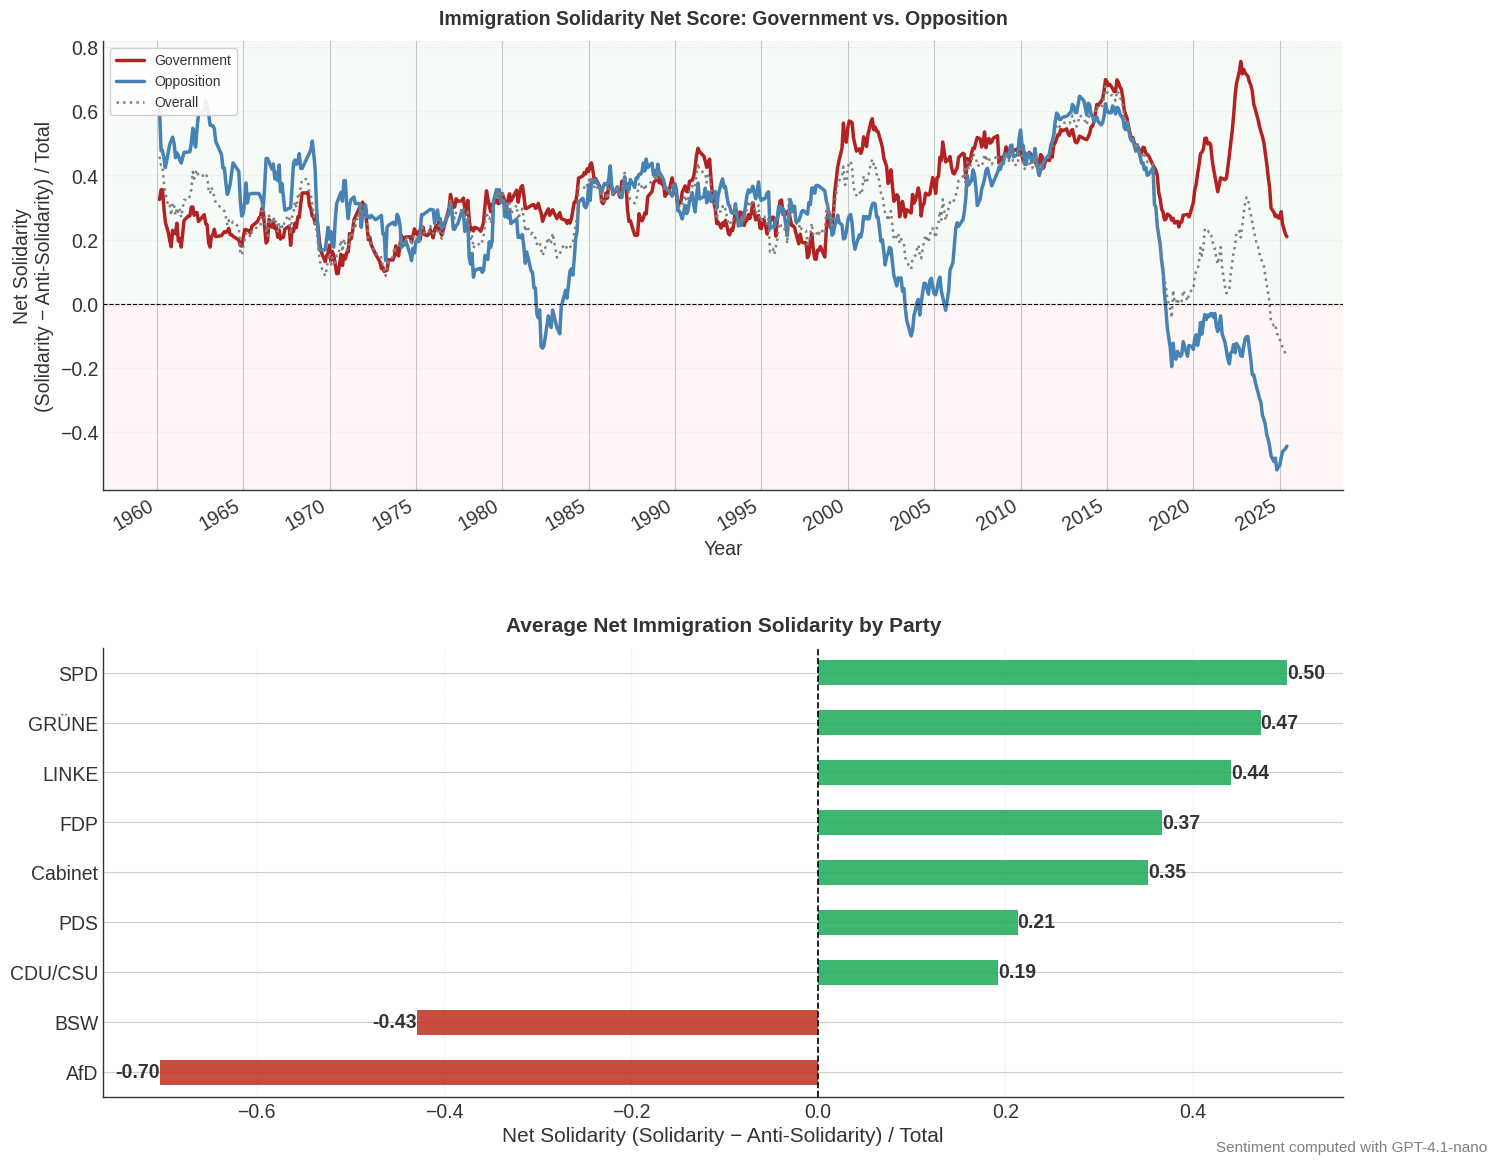
\includegraphics[width=14cm]{./../code/images/LLM/partiesGtpaverage.png}
     		\caption{\small Average Net Immigration Solidarity by Party
     			(GPT-4.1-nano).}
     		\label{fig:gpt_party_average}
     	\end{center}
     \end{figure}
     
     \begin{figure}[h]
     	\centering
     	\begin{minipage}[t]{0.45\linewidth}
     		\centering
     		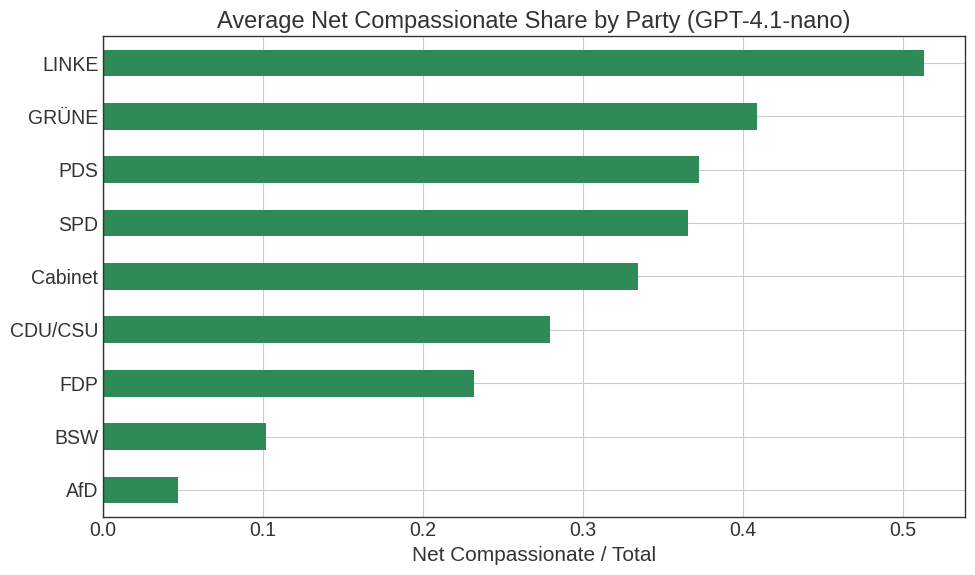
\includegraphics[width=8cm]{./images/compassion.png}
     		\caption{\small Average Net Compassionate Solidarity by Party (GPT-4.1-nano).}
     		\label{fig:gpt_compassion_party}
     	\end{minipage}
     	\hfill
     	\begin{minipage}[t]{0.45\linewidth}
     		\centering
     		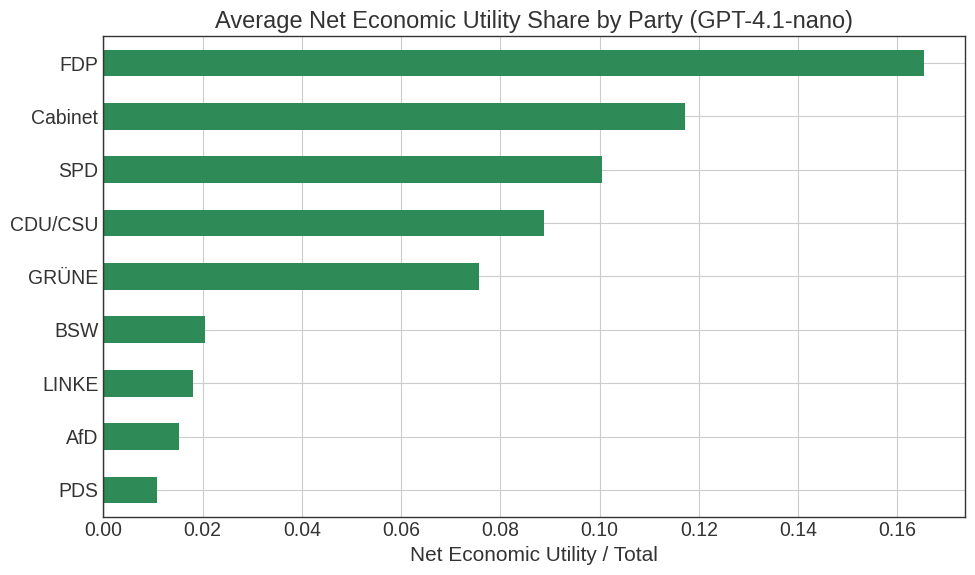
\includegraphics[width=8cm]{./images/economics.png}
     		\caption{\small Average Net Economic-Utility Solidarity by Party (GPT-4.1-nano).}
     		\label{fig:gpt_economic_party}
     	\end{minipage}
     \end{figure}
     
     We re-estimate the baseline VAR using the LLM-based opposition-sentiment series over
     three windows: 2007--2014, 2007--2019, and 2007--2025.
     
     \begin{figure}[h]
     	\begin{center}
     		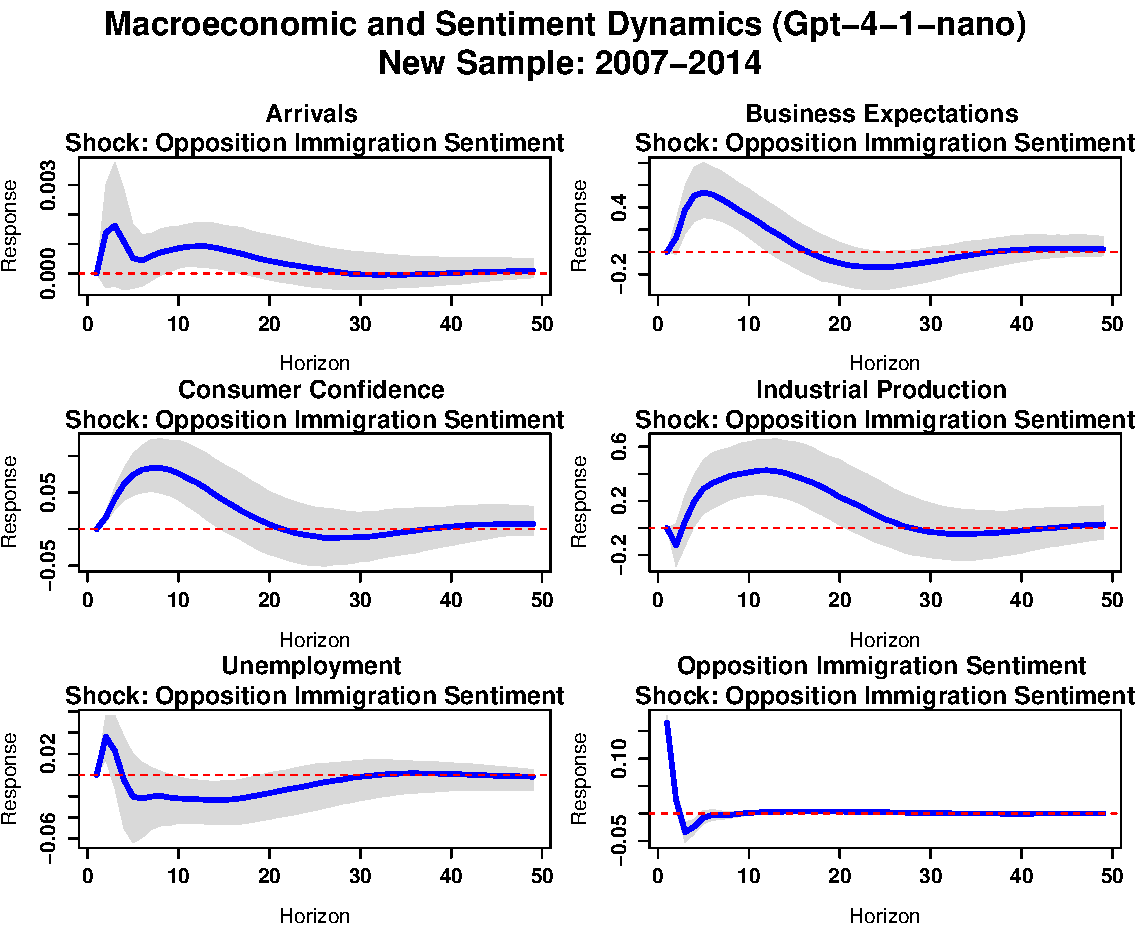
\includegraphics[width=14cm]{./../code/images/LLM/gpt_var_2007_2014.pdf}
     		\caption{\small Robustness check, LLM-based sentiment measure, sample 2007--2014. The figure shows the responses of the endogenous variables to an increase in opposition immigration sentiment, constructed using GPT-4.1-nano following \textcite{kostikova2024fine} (horizons 0--50). Shaded areas denote 68\% credible intervals. All impulse responses are obtained from a recursively identified Bayesian VAR model with two lags and Normal--Wishart priors.}
     		\label{fig:gpt_var_2007_2014}
     	\end{center}
     \end{figure}
     
     \begin{figure}[h]
     	\begin{center}
     		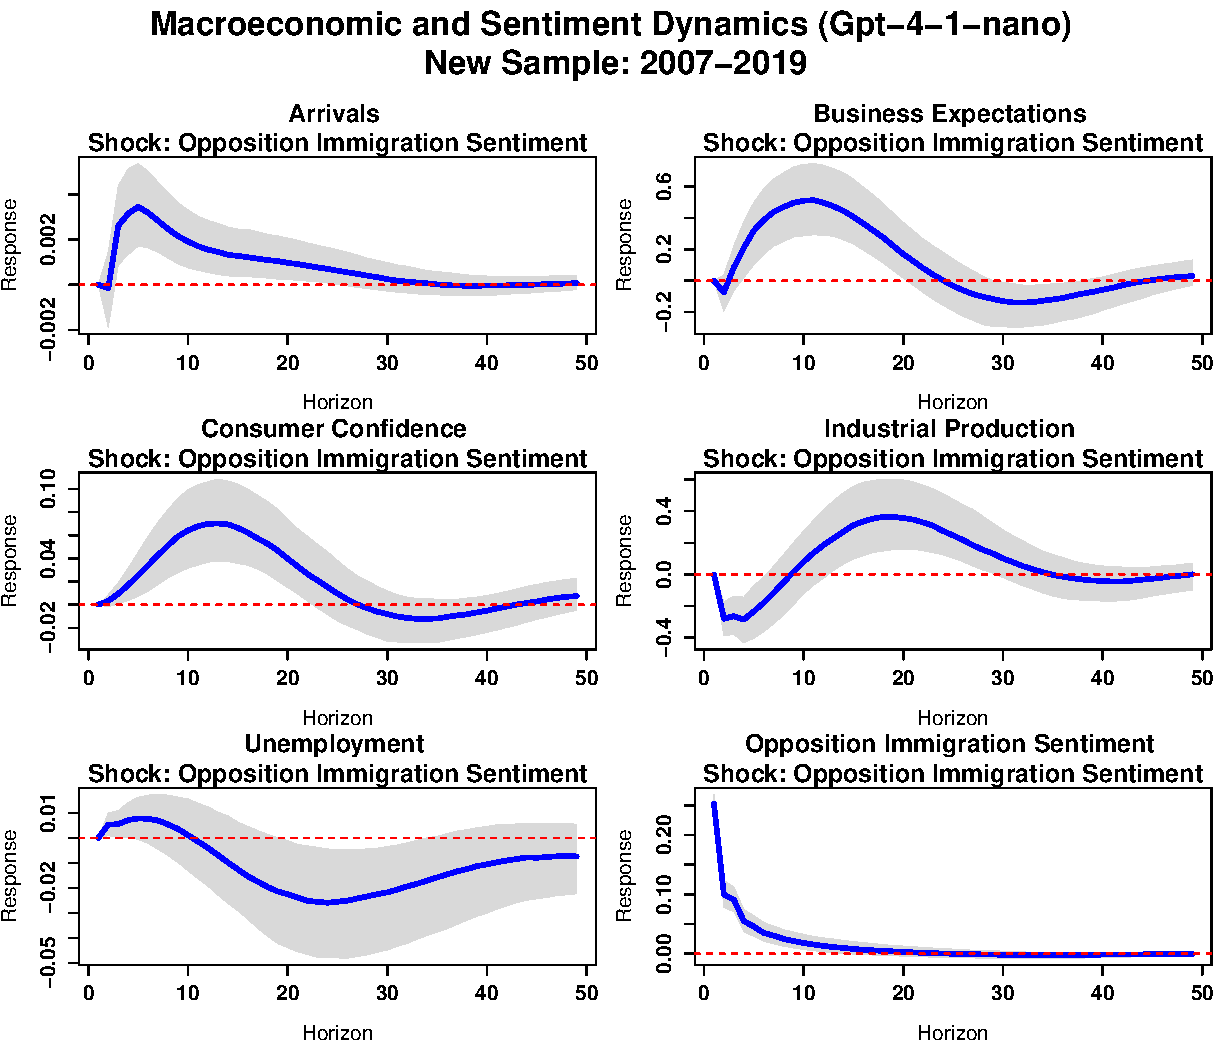
\includegraphics[width=14cm]{./../code/images/LLM/gpt_var_2007_2019.pdf}
     		\caption{\small Robustness check, LLM-based sentiment measure, sample 2007--2019. The figure shows the responses of the endogenous variables to an increase in opposition immigration sentiment, constructed using GPT-4.1-nano following \textcite{kostikova2024fine} (horizons 0--50). Shaded areas denote 68\% credible intervals. All impulse responses are obtained from a recursively identified Bayesian VAR model with two lags and Normal--Wishart priors.}
     		\label{fig:gpt_var_2007_2019}
     	\end{center}
     \end{figure}
     
     \begin{figure}[h]
     	\begin{center}
     		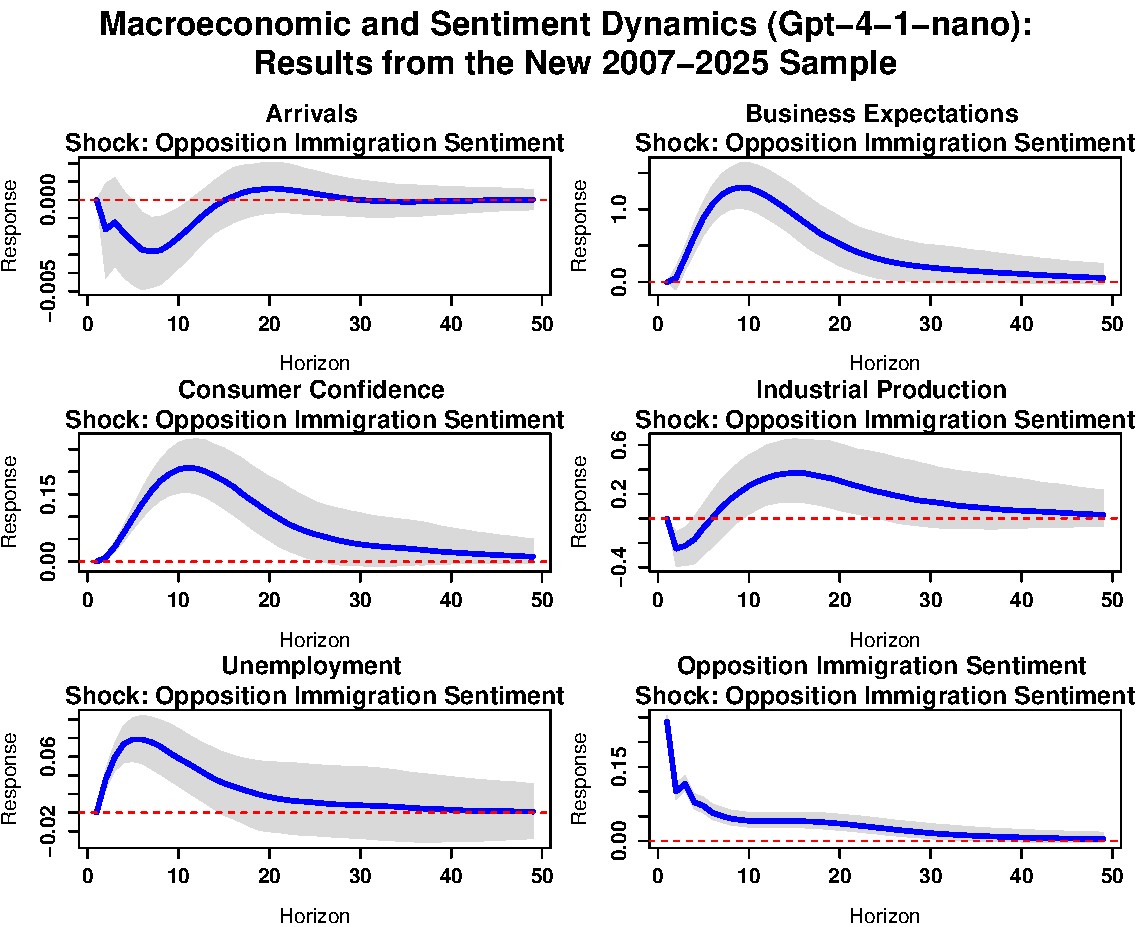
\includegraphics[width=14cm]{./../code/images/LLM/gpt_var_2007_2025.pdf}
     		\caption{\small Robustness check, LLM-based sentiment measure, sample 2007--2025. The figure shows the responses of the endogenous variables to an increase in opposition immigration sentiment, constructed using GPT-4.1-nano following \textcite{kostikova2024fine} (horizons 0--50). Shaded areas denote 68\% credible intervals. All impulse responses are obtained from a recursively identified Bayesian VAR model with two lags and Normal--Wishart priors, including a COVID-19 exogenous control dummy for observations between March 2020 and October 2021.}
     		\label{fig:gpt_var_2007_2025}
     	\end{center}
     \end{figure}
     
     Figures~\ref{fig:gpt_var_2007_2014}, \ref{fig:gpt_var_2007_2019}, and
     \ref{fig:gpt_var_2007_2025} show that opposition sentiment raises business
     expectations, consumer confidence, and industrial production. Industrial production
     does not react right away: it dips first, then turns positive. This dip lasts about
     two months in the 2007--2014 sample, six months in 2007--2019, and ten months in
     2007--2025.
     
     This pattern differs from the Doc2Vec results for 2007--2014 and 2007--2019, where
     business expectations, consumer confidence, and industrial production all *decline*
     after a sentiment shock. The likely reason is that the two sentiment series behave
     differently between 2011 and 2019: the Doc2Vec series drops sharply in this period,
     while the LLM series first rises and then falls sharply after 2014 (see
     Figure~\ref{fig:doc2vec_gpt_sentiment}). In the 2007--2025 period, the two sentiment series follow a broadly similar overall trend, which is why their impulse responses end up looking similar in shape despite differing in level. Unemployment rises after the shock, most clearly in the
     2007--2025 sample, where the response stays significant for about one and a half years.
     
     Migration arrivals behave differently across the three windows: the response is negligible in 2007--2014, significantly positive for over ten months in 2007--2019, and negative before flattening out in 2007--2025. In other words, opposition pro-immigration rhetoric had no clear effect on arrivals before 2015, a positive effect afterward — plausibly linked to the 2015--2016 refugee crisis — and a negative effect once the sample is extended to 2025, which may reflect stricter migration policy and more restrictive public rhetoric in recent years.
     
     Overall, the LLM-based sentiment measure (GPT-4.1-nano) offers a more
     context-sensitive way to capture the tone of the immigration debate, as shown by Figures~\ref{fig:gpt_party_average}, \ref{fig:gpt_compassion_party}, and
     \ref{fig:gpt_economic_party} and by the impulse responses above, consistent with \cite{kostikova2024fine}, who report a macro-F1 of 0.42 for GPT-4 on similar migration-related classification, against a human upper bound of 0.56. The differences from our dictionary-based measure are consistent with Doc2Vec's known weakness in handling negation. Finally, the fact that the impulse-response pattern is stable across samples suggests that immigration sentiment mainly works through expectation channels — business expectations and consumer confidence — while unemployment and arrivals respond more to the broader
     macroeconomic conditions of each period.
     
     Figure~\ref{fig:gpt_var_2007_2025_var} shows the forecast error variance
     decomposition: the opposition immigration sentiment shock explains about 30\% of monthly fluctuations in business expectations and consumer confidence after 10 to 15 months, but only about 5\% of the variance in unemployment after around 5 months.
     
     \begin{figure}[h]
     	\centering
     	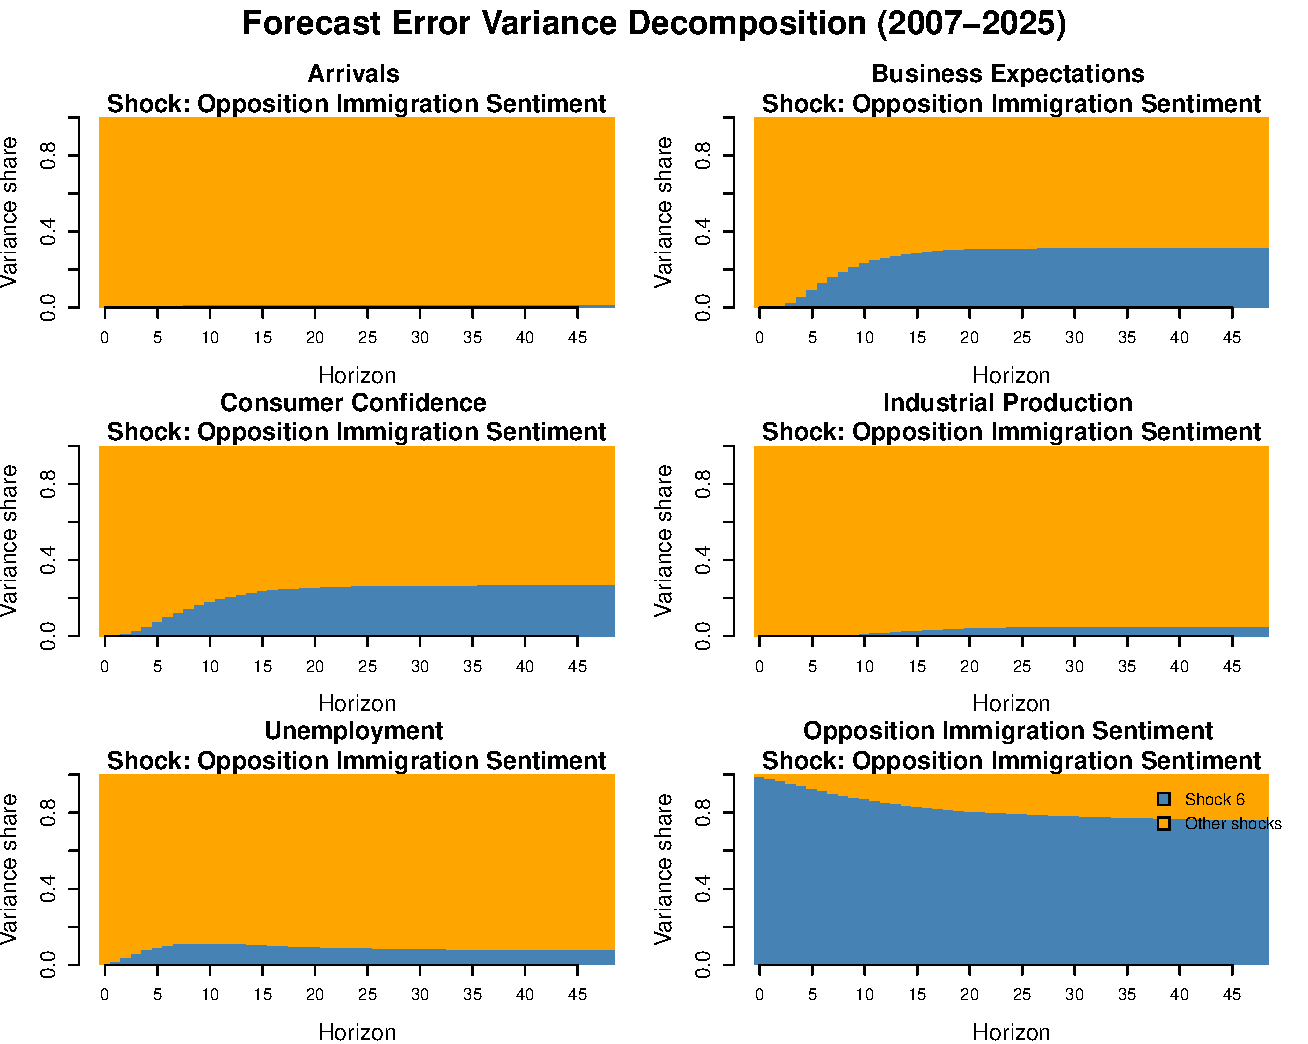
\includegraphics[width=14cm]{./../code/images/LLM/gpt_var_2007_2025Forcast.pdf}
     	\caption{Forecast Error Variance Decomposition (2007--2025) for Opposition Immigration Sentiment Shock}
     	\label{fig:gpt_var_2007_2025_var}
     \end{figure}
    
    \clearpage
    
    \section{Conclusion}
    \label{sec:conclusion}
    
    This thesis asked whether immigration-related political sentiment in the German Bundestag carries information about later macroeconomic and migration dynamics. To answer this, the analysis combined natural language processing with a Bayesian vector autoregressive (BVAR) framework. The empirical strategy first reproduced the macroeconomic setting of Maffei-Faccioli and Vella (2021) and then extended it by adding a time-varying measure of parliamentary immigration sentiment. The analysis also separated government from opposition sentiment and tested the robustness of the results across sample periods, recursive orderings, and an independent large language model (LLM)-based sentiment measure.
    
    A central methodological contribution is the construction of a dynamic immigration sentiment measure from Bundestag speeches. Instead of relying on a fixed dictionary, the approach combines manually selected seed terms with Word2Vec-based semantic expansion, PCA-guided vocabulary refinement, and rolling-window Doc2Vec representations. The rolling-window design matters because it lets the semantic representation of immigration-related language evolve over time and reduces the risk of leaking future information into the sentiment measure. The resulting index is then split into government, opposition, and aggregate Bundestag sentiment, which lets the analysis check whether political position is linked to different macroeconomic responses.
    
    The baseline BVAR results show that innovations in the dictionary-based sentiment measure are followed by movements in several macroeconomic variables. Sentiment shocks are followed by clear responses in business expectations, consumer confidence, and unemployment, while industrial production responds less strongly. Migration arrivals respond more weakly still, and this response varies across sample periods and political groups. In the reconstructed and extended samples, opposition and aggregate sentiment show especially visible responses in arrivals, unemployment, and expectations-related variables. These findings suggest that immigration-related parliamentary discourse carries economically relevant information beyond its immediate content.
    
    An important finding from the robustness checks is that the empirical relationship depends on how the sentiment measure is built. Three alternative recursive orderings for the 2007--2014 sample give qualitatively similar responses for unemployment, and to a lesser extent for arrivals, suggesting the main findings are not driven by one specific ordering choice. However, the LLM-based sentiment measure produces a different pattern for several macroeconomic variables. In particular, opposition sentiment is associated with increases in business expectations, consumer confidence, and industrial production in several specifications, while the unemployment response stays more persistent in the extended sample. Arrival responses also differ across sample periods. These differences matter because they show that conclusions about the economic content of political sentiment depend partly on how sentiment is measured.
    
    The comparison between the dictionary-based and LLM-based measures is therefore an important qualification of the results. The dictionary-based measure captures how closely parliamentary language relates to welcoming or restrictive immigration concepts, but it can be distorted by negation, reported speech, and the difference between discussing and endorsing a position. An LLM-based classifier can account for some of these contextual features more directly, though it introduces its own dependence on model choice and classification decisions. The robustness results should not be read as identifying one universally correct sentiment measure. Instead, they show that how political rhetoric is measured is itself a key part of the empirical analysis.
    
    Taken together, the evidence suggests that parliamentary immigration sentiment carries predictive information about later macroeconomic dynamics, but the size and direction of the estimated responses depend on the sentiment measure and sample period. The most persistent result across specifications is the unemployment response, while responses in expectations, industrial production, and arrivals are more sensitive to measurement and sample choice. Second, the responses of the endogenous variables to sentiment shocks built from Doc2Vec and from the LLM, using opposition speeches, show the same pattern over the larger 2007--2025 sample: a positive immigration rhetoric among opposition members is followed by more positive expectations among households and firms, while arrivals and unemployment are more sensitive to the sample period chosen.
    
    One plausible interpretation is that immigration-related rhetoric may partly reflect policymakers' reactions to prevailing economic conditions. For example, labour shortages, changes in migration pressure, or broader economic uncertainty may affect both macroeconomic indicators and how migration is discussed in parliament at the same time. In that case, a positive or welcoming sentiment shock need not be an exogenous policy move; it may instead capture a political reaction to the surrounding economic environment. The empirical design used here cannot fully separate these two mechanisms. This interpretation is offered as one possible explanation of the observed dynamics, not as a causal conclusion.
    
    The thesis also contributes to the literature by showing how political text data can be built into an established macroeconomic framework. Combining parliamentary speech analysis, dynamic semantic representations, and BVAR methods gives a framework for studying political discourse together with economic and migration variables. The government-opposition distinction further shows that parliamentary discourse should not be treated as one uniform block.
    
    Some limitations should be noted. First, the dictionary-based sentiment measure remains vulnerable to contextual features such as negation and reported speech. Second, the reconstructed macroeconomic dataset differs in some respects from the original data used by Maffei-Faccioli and Vella (2021), particularly for consumer confidence, which may explain some of the differences across replication exercises.
    
    These limitations point to directions for future work. Future research could compare several \ac{LLM}s and classification prompts under one shared validation framework. On the econometric side, richer information sets that include vacancies, wages, investment, consumption, housing prices, and net exports could help separate alternative transmission mechanisms. Nonlinear or asymmetric models could also test whether welcoming and restrictive immigration rhetoric have systematically different economic effects. Extending the analysis to other European parliaments would show whether the link between political immigration discourse and macroeconomic dynamics is specific to Germany or reflects a broader European pattern.
    
    Overall, the findings show that political discourse can be built into quantitative macroeconomic analysis in a systematic way, while also highlighting the methodological challenges of measuring political sentiment from text. The evidence supports the conclusion that immigration-related parliamentary sentiment carries economically relevant information about later macroeconomic and migration dynamics. At the same time, the sensitivity of several impulse responses to the sentiment measure and specification cautions against reading these relationships as stable structural effects. The main contribution of this thesis is therefore not to establish a simple causal link between immigration rhetoric and economic outcomes, but to build and test an empirical framework through which such relationships can be measured, compared, and studied more rigorously.
        
	\clearpage
	\addcontentsline{toc}{section}{Appendix} 					%sets header with chapter title
	\section*{Appendix}
	\markright{Appendix}
	
	\section{Unit Root and Cointegration Tables}
	% KPSS
	
	\begin{table}[htbp]
		\centering
		\caption{KPSS Tests for Level Stationarity}
		\label{tab:kpss_level}
		\begin{tabular}{p{8cm}ccc}
			\hline
			\textbf{Variable} & \textbf{KPSS} & \textbf{p-value} & \textbf{Decision} \\
			\hline
			Immigration sentiment in government speeches
			& 1.5265 & $<0.01$ & Non-stationary \\
			Immigration sentiment in opposition speeches
			& 1.7362 & $<0.01$ & Non-stationary \\
			Consumer confidence index
			& 1.9268 & $<0.01$ & Non-stationary \\
			Business expectations index
			& 0.1913 & $>0.10$ & Stationary \\
			Industrial production index
			& 1.8047 & $<0.01$ & Non-stationary \\
			Number of registered unemployed
			& 2.9381 & $<0.01$ & Non-stationary \\
			Total net migration
			& 1.7774 & $<0.01$ & Non-stationary \\
			\hline
		\end{tabular}
		
		\begin{flushleft}
			\footnotesize
			\textit{Notes:} The macroeconomic variables are based on the dataset
			employed by Maffei-Faccioli and Vella \parencite{maffei2021does},
			extended to the sample period considered in this study. The two
			political sentiment variables are constructed from parliamentary
			speeches and distinguish between government and opposition speeches.
			The KPSS test has level stationarity as the null hypothesis. The
			truncation lag parameter is 4 for all tests. The null hypothesis is
			rejected at the 5\% significance level when the p-value is below 0.05.
			Reported p-values of $<0.01$ and $>0.10$ reflect the bounds returned
			by the R implementation.
		\end{flushleft}
	\end{table}

	\begin{table}[htbp]
		\centering
		\caption{Johansen Trace Test for Cointegration}
		\label{tab:johansen_trace}
		\begin{tabular}{lrrrr}
			\hline
			\textbf{Null Hypothesis} & \textbf{Trace Statistic} &
			\textbf{10\%} & \textbf{5\%} & \textbf{1\%} \\
			\hline
			$r = 0$    & 280.88 & 126.58 & 131.70 & 143.09 \\
			$r \leq 1$ & 189.89 & 97.18  & 102.14 & 111.01 \\
			$r \leq 2$ & 117.70 & 71.86  & 76.07  & 84.45 \\
			$r \leq 3$ & 68.57  & 49.65  & 53.12  & 60.16 \\
			$r \leq 4$ & 38.55  & 32.00  & 34.91  & 41.07 \\
			$r \leq 5$ & 17.31  & 17.85  & 19.96  & 24.60 \\
			$r \leq 6$ & 3.66   & 7.52   & 9.24   & 12.97 \\
			\hline
		\end{tabular}
		
		\begin{flushleft}
			\footnotesize
			\textit{Notes:} The Johansen trace test is estimated with three lags
			($K=3$), a constant restricted to the cointegration space, and no
			deterministic linear trend. The test is applied to the seven-variable
			system including migration, business expectations, consumer confidence,
			industrial production, unemployment, government sentiment, and
			opposition sentiment. The trace test sequentially tests the null
			hypothesis of at most $r$ cointegrating relationships. At the 5\%
			significance level, the null hypotheses $r=0$, $r\leq1$, $r\leq2$,
			$r\leq3$, and $r\leq4$ are rejected, whereas $r\leq5$ cannot be
			rejected. Therefore, the results indicate a cointegration rank of
			$r=5$ among the variables.
		\end{flushleft}
		
	\end{table}
		
	\clearpage
	
	\begin{table}[htbp]
		\centering
		\caption{KPSS Tests for Level Stationarity}
		\label{tab:kpss_level_dataset2}
		\begin{tabular}{p{8cm}ccc}
			\hline
			\textbf{Variable} & \textbf{KPSS} & \textbf{p-value} & \textbf{Decision} \\
			\hline
			Immigration sentiment in opposition speeches
			& 3.2246 & $<0.01$ & Non-stationary \\
			Immigration sentiment in government speeches
			& 1.4292 & $<0.01$ & Non-stationary \\
			Consumer confidence index
			& 0.7726 & $<0.01$ & Non-stationary \\
			Business expectations index
			& 1.3439 & $<0.01$ & Non-stationary \\
			Industrial production index
			& 0.7040 & 0.0132 & Non-stationary \\
			Registered unemployment rate
			& 3.3561 & $<0.01$ & Non-stationary \\
			Number of arrivals
			& 0.9843 & $<0.01$ & Non-stationary \\
			\hline
		\end{tabular}
		
		\begin{flushleft}
			\footnotesize
			\textit{Notes:} The two political sentiment variables are constructed
			from parliamentary speeches and distinguish between government and
			opposition speeches. The KPSS test has level stationarity as the null
			hypothesis. The truncation lag parameter is 4 for all tests. The null
			hypothesis is rejected at the 5\% significance level when the p-value
			is below 0.05. Reported p-values of $<0.01$ reflect the lower bound
			returned by the R implementation.
		\end{flushleft}
	\end{table}
	
	\begin{table}[htbp]
		\centering
		\caption{Johansen Trace Test for Cointegration}
		\label{tab:johansen_trace_dataset2}
		\begin{tabular}{lrrrr}
			\hline
			\textbf{Null Hypothesis} & \textbf{Trace Statistic} &
			\textbf{10\%} & \textbf{5\%} & \textbf{1\%} \\
			\hline		
			$r = 0$    & 255.62 & 126.58 & 131.70 & 143.09 \\
			$r \leq 1$ & 179.22 & 97.18  & 102.14 & 111.01 \\
			$r \leq 2$ & 121.41 & 71.86  & 76.07  & 84.45  \\
			$r \leq 3$ & 79.56  & 49.65  & 53.12  & 60.16  \\
			$r \leq 4$ & 41.49  & 32.00  & 34.91  & 41.07  \\
			$r \leq 5$ & 18.77  & 17.85  & 19.96  & 24.60  \\
			$r \leq 6$ & 6.16   & 7.52   & 9.24   & 12.97  \\
			\hline
		\end{tabular}
		
		\begin{flushleft}
			\footnotesize
			\textit{Notes:} The Johansen trace test is estimated with three lags
			($K=3$), a constant restricted to the cointegration space, and no
			deterministic linear trend. The test sequentially evaluates the null
			hypothesis of at most $r$ cointegrating relationships. At the 10\%
			significance level, the null hypotheses $r=0$, $r\leq1$, $r\leq2$,
			$r\leq3$, $r\leq4$, and $r\leq5$ are rejected, whereas $r\leq6$
			cannot be rejected. Therefore, the results indicate a cointegration
			rank of $r=6$ among the variables.
		\end{flushleft}
	\end{table}
	
	\clearpage
	
	\section{Additional Impulse Response Figures}
	% All robustness specification IRFs
	
	\begin{figure}[h]
		\centering
		\begin{minipage}[t]{0.5\linewidth}
			\centering
			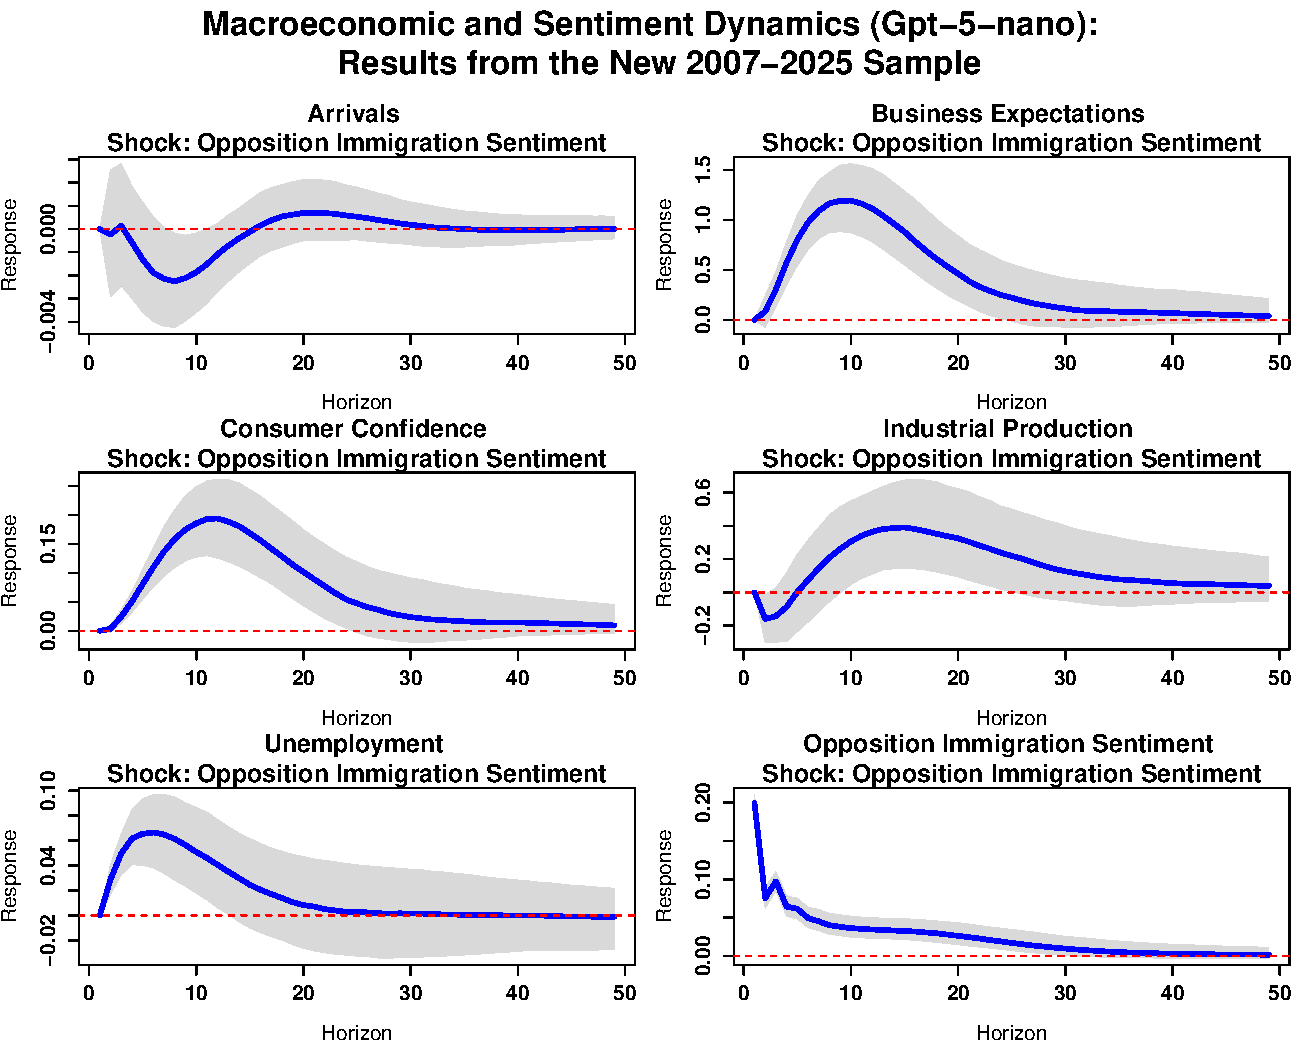
\includegraphics[width=10cm]{./../code/images/LLM/gpt5_var_2007_2025_opp_.pdf}
			\caption{GPT-5-nano, 2007--2025, opposition sentiment shock.}
			\label{fig:gpt5_opp_2007_2025}
		\end{minipage}
		\hfill
		\begin{minipage}[t]{0.5\linewidth}
			\centering
			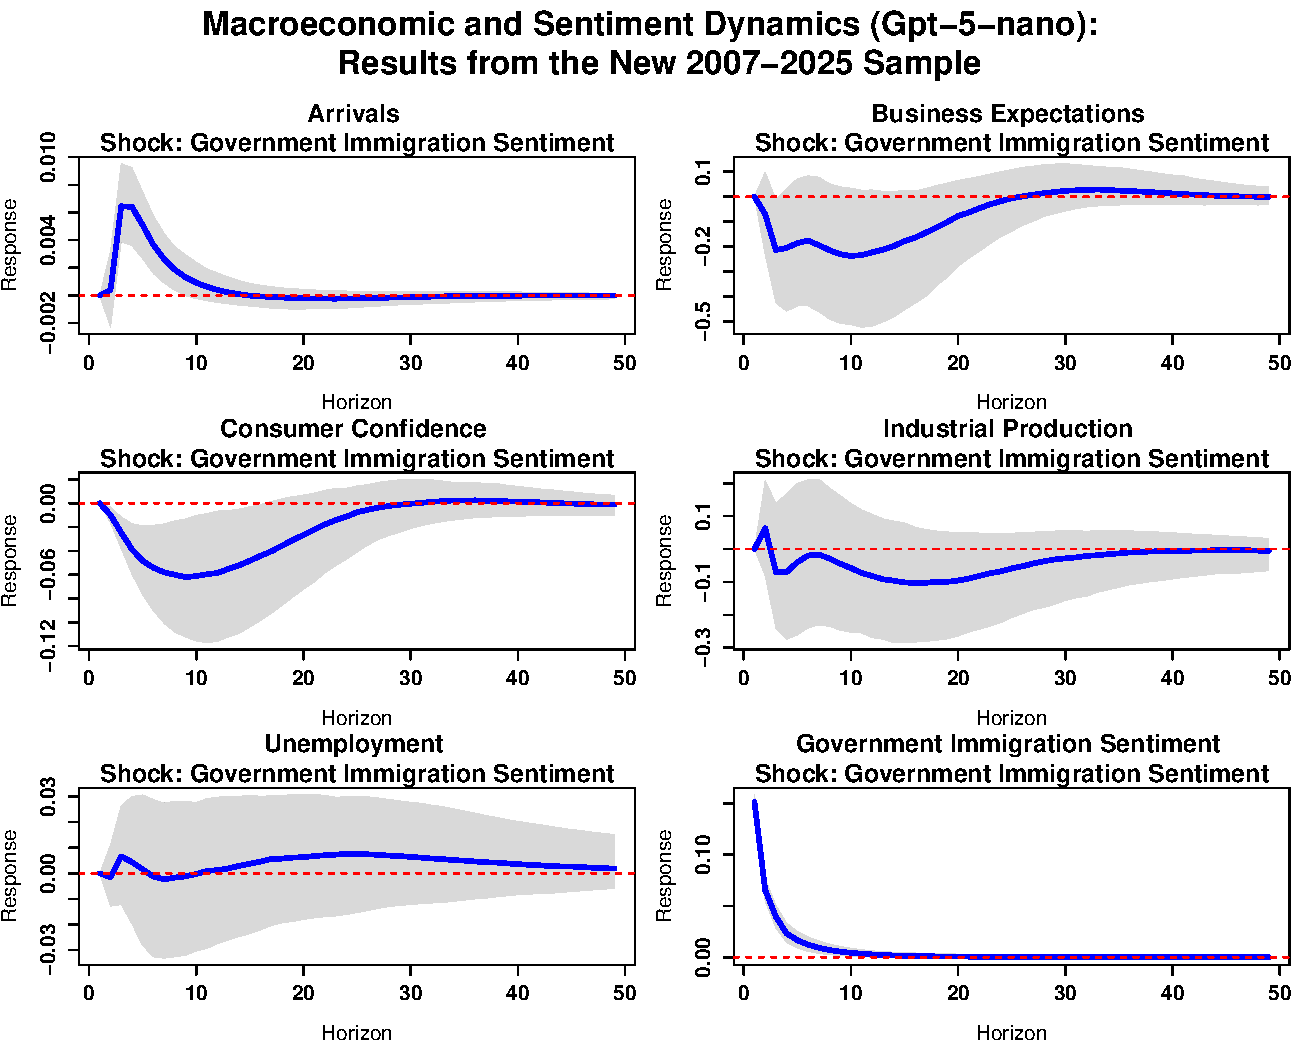
\includegraphics[width=10cm]{./../code/images/LLM/gpt5_var_2007_2025_gvt_.pdf}
			\caption{GPT-5-nano, 2007--2025, government sentiment shock.}
			\label{fig:gpt5_gvt_2007_2025}
		\end{minipage}
	\end{figure}
	
	\clearpage
	
	\section{Party-Level Sentiment Statistics}
	% Full breakdown by party, year, and episode
	\begin{figure}[htbp]
		\centering
		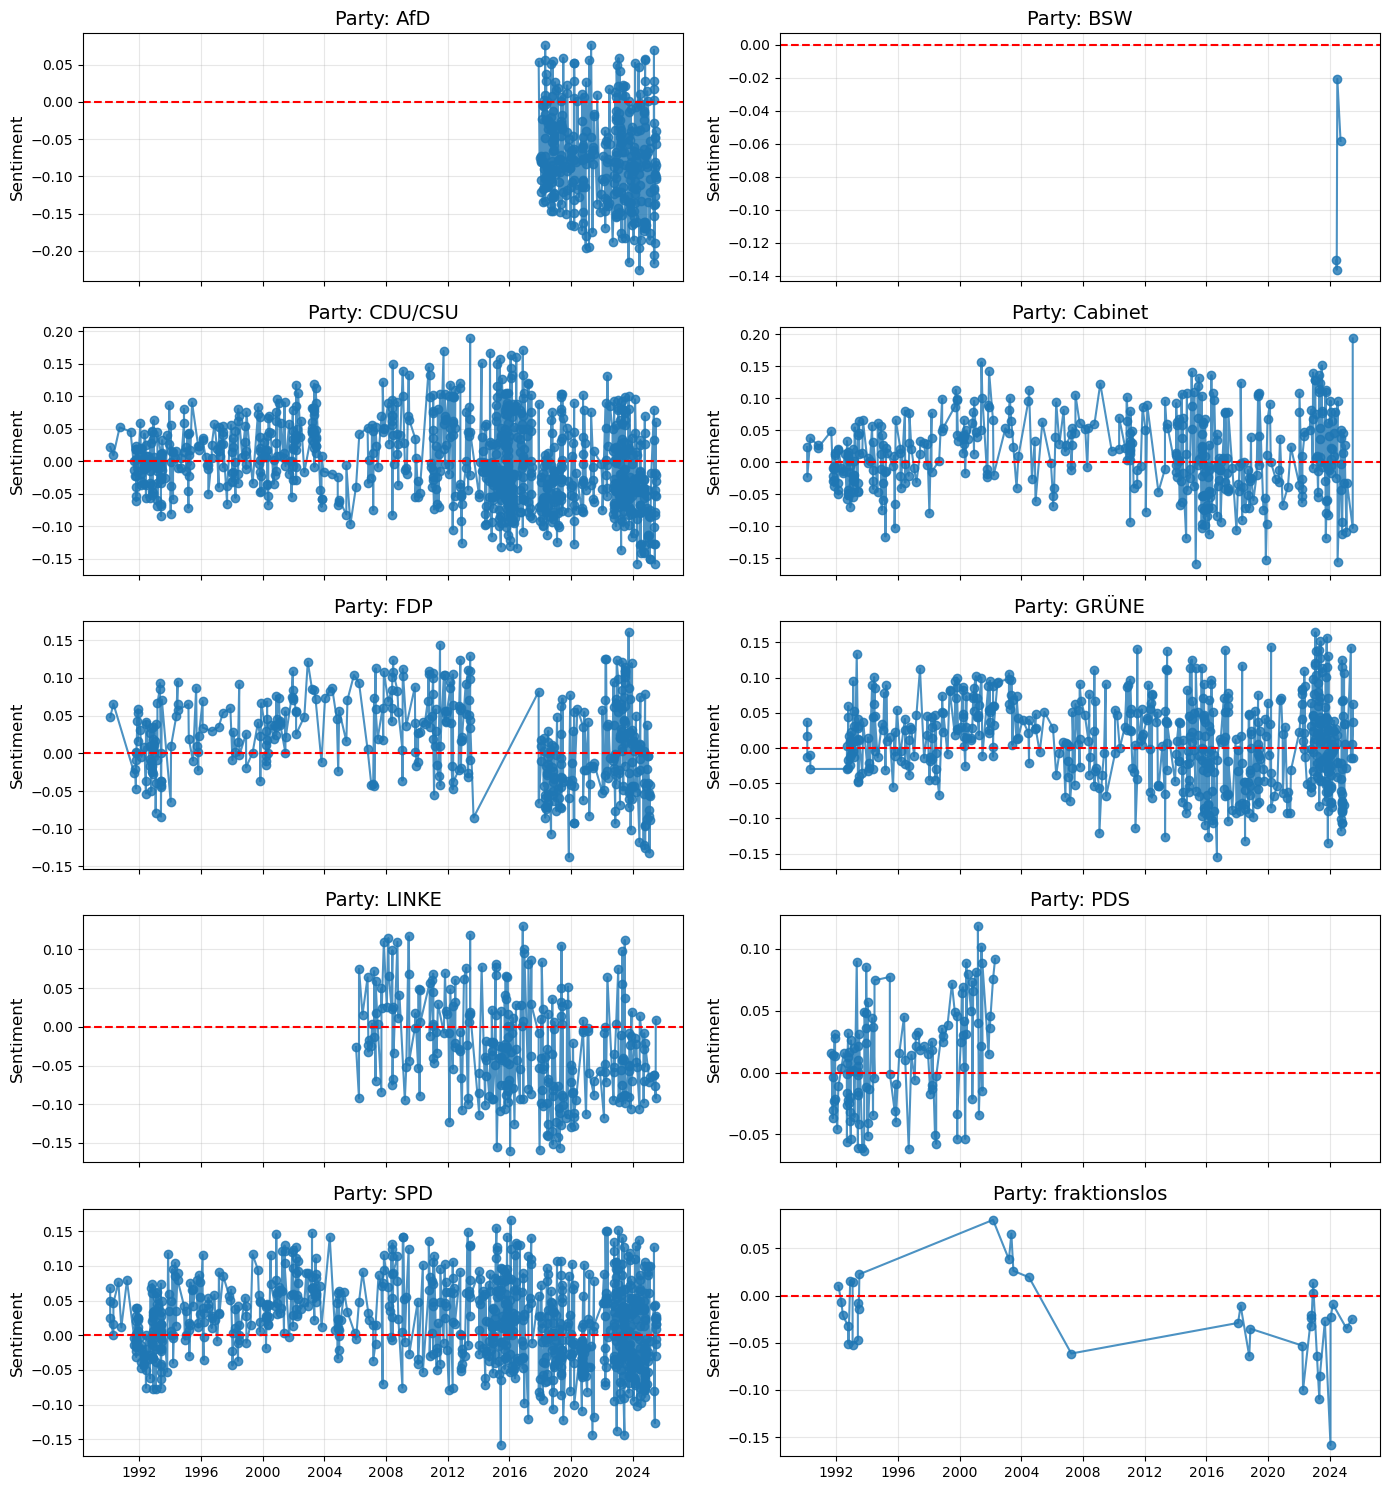
\includegraphics[width=14cm]{./../code/images/partyAveragesentiment.png}
		\caption{Evolution of Immigration Sentiment by Political Party}
		\label{fig:party_sentiment}	
		\begin{flushleft}
			\footnotesize
			\textit{Notes:} The figure presents the evolution of the estimated
			immigration sentiment scores for speeches by political party over
			the sample period. The horizontal red dashed line represents zero
			sentiment. Positive values indicate relatively pro-immigration
			sentiment, whereas negative values indicate relatively restrictive
			sentiment. The figure illustrates differences in the level and
			variability of immigration-related sentiment across parties and
			over time.
		\end{flushleft}
	\end{figure}
	
	\section{\ac{LLM} Sentiment Classification Prompt}
	\label{app:gpt_prompt}
	
	Sentiment classification via GPT-4.1-nano and GPT-5-nano was performed
	using the prompt template below, generated programmatically for each
	speech excerpt. The five solidarity and five anti-solidarity subtypes,
	defined in Table~\ref{tab:solidarity_subtypes}, are inserted into the
	template at runtime.
	
	\begin{table}[h]
		\centering
		\small
		\caption{Solidarity and anti-solidarity subtypes used in prompt construction.}
		\label{tab:solidarity_subtypes}
		\begin{tabular}{p{3.2cm}p{9.5cm}}
			\hline
			\textbf{Subtype} & \textbf{Definition} \\
			\hline
			\multicolumn{2}{l}{\textit{Solidarity}} \\
			Group-based & Migrants are recognized as a legitimate group with equal rights, interests, or claims. \\
			Exchange-based & Support is based on reciprocity: an individual migrant contributes or fulfills obligations and therefore deserves support or rights. \\
			Economic-utility & Migration is presented as beneficial or necessary for the German economy or society (e.g., labor shortages, demographics, growth, taxes, skilled labor). \\
			Compassionate & Migrants/refugees are portrayed as vulnerable or suffering and therefore deserving protection, sympathy, or support. \\
			Empathic & Migrants' identity, dignity, culture, autonomy, or self-determination is explicitly recognized or respected. \\
			\multicolumn{2}{l}{\textit{Anti-solidarity}} \\
			Group-based & Migrants are portrayed as an out-group or as having fewer rights than natives; native interests are prioritized. \\
			Exchange-based & An individual migrant is portrayed as taking more than they contribute or failing to fulfill obligations. \\
			Economic-burden & Migration is presented as economically harmful or costly (e.g., welfare costs, fiscal burden, wage competition, pressure on resources). \\
			Compassionate & Migrants' need for protection or humanitarian support is dismissed or portrayed as undeserving. \\
			Empathic & Migrants' identity, dignity, culture, autonomy, or self-determination is denied or rejected. \\
			\hline
		\end{tabular}
	\end{table}
	
	\clearpage
	
	\begin{lstlisting}[style=promptstyle, caption={Prompt template passed to the \ac{LLM} for each speech excerpt.}, label={lst:gpt_prompt}]
		Classify the following German parliamentary speech excerpt according to its
		stance toward migrants, refugees, asylum seekers, or immigrants.
		
		LABELS
		------
		SOLIDARITY = supportive, accepting, protective, inclusive, or sympathetic.
		ANTI-SOLIDARITY = opposing, excluding, rejecting, hostile, or unwilling to support.
		MIXED = both meaningful solidarity and anti-solidarity.
		NONE = no clear stance toward migrants.
		
		RULES
		-----
		- Migration must be the target. Mentioning migration alone is not enough.
		- Neutral facts, statistics, questions, or policy descriptions = NONE.
		- Criticism/support of government or migration policy is not automatically
		anti/pro-migration; classify only the stance toward migrants.
		- Do not classify unrelated groups or historical German expellees as migrants.
		- If the evidence is unclear, choose NONE.
		- If SOLIDARITY or ANTI-SOLIDARITY, choose exactly ONE subtype.
		- If MIXED or NONE, subtype = NONE.
		
		SOLIDARITY SUBTYPES
		-------------------
		[inserted from Table~\ref{tab:solidarity_subtypes}]
		
		ANTI-SOLIDARITY SUBTYPES
		------------------------
		[inserted from Table~\ref{tab:solidarity_subtypes}]
		
		TEXT
		----
		**<speech excerpt>**
		
		OUTPUT FORMAT
		-------------
		
		Return EXACTLY two lines and nothing else:
		
		Justification: <one short sentence explaining the decision>
		Label: <HIGH-LEVEL>[-<SUBTYPE>]
		
		VALID LABELS
		------------
		
		SOLIDARITY-GROUP-BASED
		SOLIDARITY-EXCHANGE-BASED
		SOLIDARITY-ECONOMIC-UTILITY
		SOLIDARITY-COMPASSIONATE
		SOLIDARITY-EMPATHIC
		
		ANTI-SOLIDARITY-GROUP-BASED
		ANTI-SOLIDARITY-EXCHANGE-BASED
		ANTI-SOLIDARITY-ECONOMIC-BURDEN
		ANTI-SOLIDARITY-COMPASSIONATE
		ANTI-SOLIDARITY-EMPATHIC
		
		MIXED
		NONE
	\end{lstlisting}

	\clearpage
	\addcontentsline{toc}{section}{Bibliography} 	%sets header with chapter title
	\printbibliography
	
	\clearpage
	\section*{Declaration of originality}
	\thispagestyle{empty}
	I hereby declare that I have written this Masterthesis independently and without using other than the indicated sources and aids and that I have identified the passages taken verbatim or in content from the used sources as such. The work in the same or similar form has not been submitted to any other examination authority.
	\\[1cm]
	Linden, 01.09.2026
	\\[1.5cm]
	Esdras Shaa Prombo
	
\end{document}
